% Generated body; only mechanical merging changes.




% s01_summary.tex (HT1dPert)
\section{Summary}\label{htp:sec:summary}
This note documents every perturbative Hamiltonian-truncation (HT) number quoted in the paper \emph{The long-range Ising
CFT: perturbative and nonperturbative approaches} and in its Supplemental Material, and how to
reproduce each from the folder \code{HT\_Pert/} of the public repository. The truncation at finite coupling is
documented separately, in the note \emph{Hamiltonian truncation of the long-range Ising model at finite coupling}
(folder \code{HT/}).

The method expands the truncated Hamiltonian of the $\phi^4$-deformed generalized free field in $\eps=2s-d$ at fixed
cutoff. Two exact relations fix the couplings, the gap $\DE=\sum_nC_n(\Lambda)\eps^n$ follows order by order, and the
coefficients are extrapolated in the cutoff (Section~\ref{htp:sec:method}). Two observations recur. First, in every
dimension, truncating the total energy or level of a state leaves it a vacuum window that does not close as the cutoff
grows. A window correction with no free parameter removes the resulting bias. In $d=1$, with it, post hoc fits of the exact
sums give $C_4$ and $C_5$ to $\HTpCfiveOneDev$ or better, and the solver data give $C_4$ to $C_7$ to
$\HTpCsevenOneDev$ or better. In $d=2$ it
works through $\eps^4$, and through $\eps^5$ with two further rules that are not derived in full. In $d=3$ it works
through $\eps^4$, with $\eps^5$ provisional. It removes the $\eps^2$ violation of the descendant spacings in all three dimensions
(in $d=3$ for the one state tested), and the $\eps^3$ violation in the single-state sectors of $d=1$; in $d=2$ it
removes at least $\HTpTwoIdentThree\%$ of the $\eps^3$ violation of single-quantum descendants at $L=14$ and 16. Second, convergence is slow: the corrections fall like
$\Lambda^{-1/2}$ times powers of $\log\Lambda$ in $d=1$ and like $1/L$ times powers of $\ln L$ in $d=2$ and $d=3$, so the
tail model carries a large part of every limit and dominates the error. Section~\ref{htp:sec:refvals} gives the reference
values (Table~\ref{htp:tab:refvals}), the deviation $\delta=|C_n^{\rm HT}/C_n-1|$ and the status words used below.

\paragraph{One dimension (Section~\ref{htp:d1:sec}).} $C_2$ and $C_3$ come from exact sums over intermediate states to
$\Lambda=\HTpOneLexact$, with a fit rule fixed in advance: $\delta=\HTpCtwoOneDev$ and $\HTpCthreeOneDev$. The same
sums extend $C_4$ to $\Lambda=\HTpOneLexact$ and $C_5$ to $\NOneCfiveLmax$, and fits frozen before the largest runs
predict them to $10^{-9}$. The frozen $C_4$ fits land $\HTpCfourOneDev$ from the exact value, with the basis and the
median chosen post hoc. Fixing the $\log^3$ tail of $C_5$ by the exponentiated $C_4$ tail gives $C_5$ to
$\HTpCfiveOneDev$, post hoc. With the complete window, the solver data to $\Lambda=\HTpLamThermal$ give $C_6$ to
$\HTpCsixOneDev$ and $C_7$ to $\HTpCsevenOneDev$, with fit windows and tail models chosen after the data were seen. The
same data give a $C_4$ range that lies below the exact value and excludes it (largest deviation
$\NOneCfourSolverDev$) and a $C_5$ range that contains it (largest deviation $\NOneCfiveSolverDev$). $C_8$ lies $\HTpCeightOneDev$ from the reference, inside its
uncertainty, when the tail models are calibrated on $C_6$ and $C_7$.

\paragraph{Two dimensions (Section~\ref{htp:d2:sec}).} The complete window, built from the level left to each counterterm,
removes the $\ln L$ divergence of $C_4$. $C_2$ to $C_4$ agree with the continuum values to better than
$\HTpTwoLowDev$, and $C_5$ to $\HTpCfiveTwoDev$, if the $C_5$ data carry no residual $\ln L$ term. The data cannot exclude one; with
the bound judged from the median of the fits it would move $C_5$ by up to about $\HTpCfiveTwoLog$, and the spread of
single fits would allow $-0.7$ to $+0.5$. $C_6$ to $C_8$ are not reproduced.

\paragraph{Three dimensions (Section~\ref{htp:d3:sec}).} With the complete window of $d=2$ carried over unchanged, exact sums
over intermediate states ($C_2$ to $L=\HTpThreeLwin$, $C_3$ and $C_4$ to $L=\HTpThreeLfour$) reproduce $C_2$
($\HTpCtwoThreeDigits$ digits), $C_3$ ($\delta=\HTpCthreeThreeDev$) and $C_4$ ($\delta=\HTpCfourThreeDev$). $C_5$, from
$L\le\HTpThreeLfive$, gives $\HTpCfiveThree$ against $-5.850$ (provisional and calibrated on $C_4^{(3)}$; a term in
$L^{-1/2}$ that $L\le\HTpThreeLfive$ cannot exclude would lower it by 0.5 to 1). The vacuum window alone diverges at
order $\eps^4$. $C_6$ to $C_8$ are not reproduced.

Section~\ref{htp:sec:repro} maps every number to its code, records, command and tolerance.

% s02_method.tex (HT1dPert): model, cutoffs, perturbation theory, tails and windows, common to d = 1, 2, 3.
\section{Model, cutoffs and perturbation theory}\label{htp:sec:method}

\subsection{Model and observable}
The long-range Ising critical point in $d$ dimensions is described by the generalized free field (GFF) $\phi$ with
nonlocal kinetic term $\phi(-\partial^2)^{s/2}\phi$, deformed by a $\phi^4$ interaction
\cite{htp:Fisher:1972zz,htp:Sak:1973oqx,htp:Paulos:2015jfa}. With $\eps=2s-d$ the field dimension is
\begin{equation}
 \Ds=\frac{d-s}{2}=\frac{d-\eps}{4},
\end{equation}
exactly, since no local counterterm renormalizes the nonlocal kinetic term \cite{htp:Paulos:2015jfa}. The nonlocal
equation of motion gives the shadow relation $\Delta_{\phi^3}=d-\Ds$ \cite{htp:Paulos:2015jfa}. These two exact statements
are the only physics inputs of the truncation: they fix the two couplings of the Hamiltonian order by order. The
observable is the thermal operator $\varepsilon=[\phi^2]$,
\begin{equation}
 \DE(\eps)=\sum_{n\ge0}C_n\eps^n,\qquad C_0=\frac d2,\qquad C_1=-\frac16 .
 \label{htp:eq:Cn}
\end{equation}
We write $C_n(\Lambda)$ or $C_n(L)$ for a coefficient computed at finite cutoff, and $C_n$, or $C_n^{(d)}$ where the
dimension must be named, for the continuum value.

\subsection{Reference values and conventions}\label{htp:sec:refvals}
Table~\ref{htp:tab:refvals} lists the continuum coefficients that the HT results are compared with. They come from the
$\eps$ expansion of the GFF with Feynman graphs. The note \emph{Thermal dimensions in the long-range Ising model}, in
the folder \code{GFF/} of the public repository, documents them, and the paper \emph{The long-range Ising
CFT: perturbative and nonperturbative approaches} summarizes them. In this note they are used only for
comparison, except where a fit is explicitly labeled as calibrated on them.

\begin{table}[ht]
\centering\footnotesize\renewcommand{\arraystretch}{1.2}
\begin{tabular}{@{}clll@{}}
\toprule
 & $d=1$ & $d=2$ & $d=3$ \\
\midrule
$C_2$ & $\tfrac19(\pi+4\log2)=0.657131263981$ & $\tfrac49\log2=0.308065413582$ & $\tfrac19(2+4\log2-\pi)=0.181221785405554$ \\
$C_3$ & $-3.719856322902$ & $-0.874850012653$ & $-0.353581520433$ \\
$C_4$ & $45.42488010356$ & $5.048868431$ & $1.228063545$ \\
$C_5$ & $-731.13947662454$ & $-38.833645896$ & $-5.850351421$ \\
$C_6$ & $14331.68703275805$ & $362.366\pm0.004$ & $33.5754\pm0.0005$ \\
$C_7$ & $-322550\pm41$ & $-3876.1\pm2.1$ & $-220.35\pm0.13$ \\
$C_8$ & $(8.060\pm0.017)\times10^6$ & $45990\pm33$ & $1602.6\pm3.9$ \\
\bottomrule
\end{tabular}
\caption{Continuum coefficients $C_n^{(d)}$ used as references, from the GFF note (folder \code{GFF/}). $C_2$ to
$C_5$ are closed forms, and $C_6^{(1)}$ is a finite representation in special-function values (an independent sum over
all six-loop graphs gives $14331.6870328(5)$). The other entries are Monte Carlo estimates; their $\pm$ is the empirical
allowance of the GFF note, about four to five sampling standard errors, not a standard deviation.}
\label{htp:tab:refvals}
\end{table}

\paragraph{Conventions.} The deviation of an HT value from the reference is $\delta=|C_n^{\rm HT}/C_n-1|$; for a range,
$\delta$ is the largest deviation of its ends. Quoted HT uncertainties are spreads over fit models, fit windows or
prescriptions, not standard errors; values are rounded with the PDG rule. Each result carries the status word of the
analysis that produced it. The words are \emph{final} (the analysis is complete; it may still contain post hoc
choices), \emph{blind} (fit rules fixed before the data they predict existed), \emph{post hoc} (a choice
made after the data, or the continuum value, were seen), \emph{calibrated} (tail models selected by their reproduction of
known continuum coefficients), \emph{provisional}, or \emph{not reproduced}.

\subsection{Radial quantization and the Hamiltonian}
In radial quantization the GFF is a set of free oscillators. In $d=1$ the ``sphere'' is the pair of points
$\sigma=\pm1$ and
\begin{equation}
 \phi_\sigma=\sum_{n\ge0}u_n\,\sigma^n\big(a_n+a_n^\dagger\big),\qquad
 u_n^2=\frac{(2\Ds)_n}{n!}=\frac{\big(\tfrac{1-\eps}2\big)_n}{n!},\qquad E(a_n^\dagger)=\Ds+n .
 \label{htp:eq:modes}
\end{equation}
With the level $\ell=\sum_n nN_n$ and the particle number $P=\sum_nN_n$,
\begin{equation}
 H=H_0+\eps F_1+r(\eps)\,M+g(\eps)\,V,\qquad H_0=\ell+\tfrac P4,\qquad F_1=-\tfrac P4,
 \label{htp:eq:H}
\end{equation}
where $M=\langle{:}\phi^2{:}\rangle$ and $V=\tfrac1{12}\langle{:}\phi^4{:}\rangle$ are averages over the sphere, normal
ordered. Their matrix elements are used as they stand in the truncated space: operators are never commuted past each
other, because in a truncated space a commutator identity no longer holds. The sphere average keeps only transitions
that change $\ell$ by an even amount, so the parity of $\ell$ is conserved; the reference states below have $\ell=0$, and
odd-$\ell$ states such as $\partial\phi$ enter only the descendant tests. The field parity $(-1)^P$ is conserved as
well. $\eps$ enters only through $u_n(\eps)$ and $F_1$; the Taylor coefficients of $u_n$ are kept exactly to the working
order. The $d=2$ and $d=3$ mode functions and weights are given in Sections~\ref{htp:d2:sec} and~\ref{htp:d3:sec}.

\subsection{Cutoffs}
\paragraph{$d=1$: frozen energy cutoff.} The Fock space keeps the states whose energy at $\eps=0$ satisfies
\begin{equation}
 E^0=\ell+\tfrac P4\le\Lambda\qquad\Longleftrightarrow\qquad 4\ell+P\le4\Lambda ,
 \label{htp:eq:Lambda}
\end{equation}
and the thresholds are not moved with $\eps$. Energies at $\eps=0$ are multiples of $\tfrac14$.

\paragraph{$d=2,3$: level cutoff.} The zero mode (the mode with the lowest energy, $\Ds$) is kept untruncated; the
other modes form the bath, whose total level is cut at $L$: $\ell\le L$ in $d=2$, $N_b\le L$ in $d=3$
(Sections~\ref{htp:d2:sec}, \ref{htp:d3:sec}).

\subsection{Tuning and the coefficients}\label{htp:sec:tuning}
The reference states are the zero-mode states $|p\rangle=(a_0^\dagger)^p|0\rangle/\sqrt{p!}$ with $\ell=0$: $p=0$ is
the vacuum, $p=1$ and $p=3$ are $\phi$ and $\phi^3$, $p=2$ is $\phi^2$, and $p=6$ ($\phi^6$) gives the gap channel used
for the tail exponents. The couplings $r=\sum_{k\ge1}r_k\eps^k$ and $g=\sum_{k\ge1}g_k\eps^k$ are fixed order by order by
\begin{equation}
 E_1-E_0=\Ds,\qquad E_3-E_0=d-\Ds,\qquad \DE=E_2-E_0=\sum_nC_n(\Lambda)\eps^n .
 \label{htp:eq:tune}
\end{equation}
At $\eps=0$, $\langle p|M|p\rangle-\langle0|M|0\rangle=2p$ and $\langle p|V|p\rangle-\langle0|V|0\rangle=p(p-1)/2$, so
the solve is triangular. At first order $r_1=0$ and $g_1=\tfrac13$, so $C_0=\tfrac d2$ and $C_1=-\tfrac16$ at every
cutoff. With $\mathcal E_p$ the order-$\eps^n$ energy of $|p\rangle$ without the $r_n$, $g_n$ terms,
\begin{equation}
 C_n=\mathcal E_2-\mathcal E_1-\tfrac13\big(\mathcal E_3-\mathcal E_0\big)=-\tfrac13\,\Delta_p^3\mathcal E_p\qquad(n\ge2):
 \label{htp:eq:Pi}
\end{equation}
shifts linear or quadratic in $p$ are absorbed by $r$ and $g$.

\paragraph{Evaluation.} The $\eps$ series are computed by formal power-series algebra at fixed cutoff, never by
sampling $\eps$. At low orders a Rayleigh--Schr\"odinger recursion on truncated power series in $\eps$ gives the wave
functions. At high orders a trial state correct through $\eps^k$ (order $k$) gives the energy through $\eps^{2k+1}$ by
its Rayleigh quotient, and the eighth order adds one scalar term (Section~\ref{htp:d1:sec:data}). At order $k$ no
intermediate state of $|p\rangle$ has more than $p+4k$ particles, or more than $4k$ particles in modes $n\ge1$, so these
particle caps are exact at the order computed. Independently, the order-$n$ Rayleigh--Schr\"odinger expressions can be
summed exactly over the intermediate states of the truncated Hamiltonian, grouped by the levels of the intermediate
states between consecutive vertices, without building a basis. This gives $C_2$ to $C_4$ to $\Lambda=2000$ and $C_5$ to
$\Lambda=500$ in $d=1$, $C_4$, $C_5$ to large $L$ in $d=2$, and $C_2$ to $C_4$ to $L=600$ and $C_5$ to $L=40$ in $d=3$.

\subsection{Large-cutoff tails}\label{htp:sec:tails}
At second order the $d=1$ truncation has a closed form: at every cutoff
\begin{equation}
 C_2(\Lambda)=\!\!\sum_{\substack{n\ {\rm even}\\0\le n\le\Lambda-2}}\!\!\bar u_n^2\Big[\frac{2}{81(n-\frac12)}+\frac{2}{9(n+\frac12)}
 +\frac{2}{81(n+1)}+[n>0]\frac{2}{9n}\Big],\qquad \bar u_n^2=u_n^2\big|_{\eps=0}=\frac{(1/2)_n}{n!},
 \label{htp:eq:C2shell}
\end{equation}
which every solver run checks, and its tail is
\begin{equation}
 C_2(\Lambda)-C_2\simeq-\frac{40}{81\sqrt\pi}\,\Lambda^{-1/2}=-0.2786121\,\Lambda^{-1/2} .
 \label{htp:eq:T2}
\end{equation}
Cutoff effects scale as $\Lambda^{-(\Delta_{\rm irr}-1)}$ with $\Delta_{\rm irr}$ the dimension of the leading
irrelevant operator, $\phi^6$. Its gap $\Delta_6=E_6-E_0$, computed in the same truncation, defines
\begin{equation}
 \omega(\eps)=\Delta_6(\eps)-1=\tfrac12+\tfrac72\eps+\sum_{k\ge2}\omega_k\eps^k,
 \label{htp:eq:omega}
\end{equation}
with $\omega_1=-\tfrac64+15g_1=\tfrac72$ from the one-loop rule $[\eps]\Delta_{\phi^n}=-\tfrac n4+\binom n2g_1$, the same
rule that gives $C_1=-\tfrac16$ for $n=2$. The tail model of the extrapolations is
\begin{equation}
 \sum_n\big[C_n(\Lambda)-C_n\big]\eps^n=\Lambda^{-1/2}\Big(\sum_{n\ge2}a_n\eps^n\Big)\,e^{-[\omega(\eps)-\frac12]\log\Lambda}
 +\rho(\eps,\Lambda),
 \label{htp:eq:tail}
\end{equation}
with the remainder $\rho$ built from the terms $\Lambda^{-p}\log^j\Lambda$ of one of six bases fixed in advance:
\begin{center}\footnotesize
\begin{tabular}{@{}cl@{}}
\toprule
basis & terms $(p,j)$ of $\rho$ \\
\midrule
A & $(1,0)$, $(\tfrac32,0)$, $(\tfrac32,1)$, $(2,0)$ \\
B & A and $(2,1)$ \\
C & $(1,0)$, $(1,1)$, $(\tfrac32,0)$, $(\tfrac32,1)$ \\
D & C and $(2,0)$ \\
E & D and $(2,1)$ \\
F & $(1,0)$, $(\tfrac32,0)$, $(\tfrac32,1)$, $(\tfrac32,2)$, $(2,0)$ \\
\bottomrule
\end{tabular}
\end{center}
The model is fitted order by order, with $C_2$ and $C_3$ fixed to their continuum values and $C_4$ to $C_8$ fitted in
sequence. Identifying the gap with the leading irrelevant operator is an assumption for this regulator.

\paragraph{Top logarithm.} If the $\Lambda^{-1/2}$ tail comes from a single channel whose amplitude starts at $\eps^2$,
Eq.~\eqref{htp:eq:tail} fixes the coefficient of the highest power of $\log\Lambda$ at each order:
\begin{equation}
 C_n(\Lambda)-C_n\ni c_n\,\Lambda^{-1/2}\log^{n-2}\Lambda,\qquad
 c_n=a_2\frac{(-\omega_1)^{n-2}}{(n-2)!},\qquad a_2=-\frac{40}{81\sqrt\pi},
 \label{htp:eq:toplog}
\end{equation}
independently of $\omega_{k\ge2}$, of $a_{k\ge3}$ and of channels that start at $\eps^3$ or later. The exact sums test it:
$c_3$ agrees to $\NOneTopLogThree$ and $c_4$ to $\NOneTopLogFour$ (Section~\ref{htp:d1:sec:exact}).

\subsection{The vacuum window}\label{htp:sec:window}
Truncating the total energy of a state makes the cutoff effectively nonlocal and state dependent~\cite{htp:Rychkov:2014eea}.
In $\phi^4$ theory in $2+1$ dimensions this spoils the cancellation of disconnected vacuum bubbles in Hamiltonian
perturbation theory and gives new UV divergences, which Ref.~\cite{htp:Elias-Miro:2020qwz} addressed with perturbative
state-dependent counterterms that add back the missing states.
A basis state of energy $E^0_i$ is dressed only by vacuum bubbles with $E_b\le\Lambda-E^0_i$, while the vacuum keeps all
bubbles with $E_b\le\Lambda$, so the state misses
\begin{equation}
 E_b\in\big(\Lambda-E^0_i,\Lambda\big],\qquad N_{{\rm w},i}=\#\big\{\text{odd }k\in(\Lambda-E^0_i,\Lambda]\big\}.
 \label{htp:eq:window}
\end{equation}
At $\eps=0$ every four-particle shell of odd energy $k$ carries $-g^2/6$, so the deficit is proportional to the number
$N_{\rm w}$ of missing shells, which is of order one at every cutoff and does not decay as $\Lambda\to\infty$. The
descendant spacings $v_n(\mathcal O)=E(\partial^n\mathcal O)-E(\mathcal O)-n$, which vanish in a conformal theory,
measure it: raw HT gives $v_n=\tfrac{N_{\rm w}}{54}\eps^2+O(\eps^3)$.

\paragraph{Complete window, $d=1$.} We add to every basis state $m$ the diagonal shift
\begin{equation}
 D^{\rm conn}_m=E_c(\Lambda)-E_c\big(\lfloor\Lambda-E^0_m\rfloor_{1/2}\big),
 \label{htp:eq:Dconn}
\end{equation}
with $\lfloor\cdot\rfloor_{1/2}$ the half-integer floor and $E_c(x)$ the vacuum energy at cutoff $x$ of the truncated
Hamiltonian plus the same correction, and retune $r$ and $g$. Since $D^{\rm conn}_{s+b}=D^{\rm conn}_s+D^{[\Lambda-E_s]}_b$
for a disconnected bubble $b$, each window is restored exactly once; the literal vacuum-energy difference
$E_{\rm vac}(\Lambda)-E_{\rm vac}(\Lambda-E^0_m)$ would count the bubble-bubble class twice. There is no free parameter.
At second order in $g$, $D^{\rm conn}$ reduces to the isolated window $g^2D$ of the second-order vacuum bubbles, the
counterpart of Patch~I of Ref.~\cite{htp:Elias-Miro:2020qwz}: a state-dependent counterterm that adds back the same missing
four-particle states, with the unperturbed energy of the level being computed in its energy denominator, where $g^2D$
has the bubble energy alone. Its Patch~II, called a temporary fix there, restores towers of iterated bubbles up to five bubbles with every bubble cut at the full cutoff; $D^{\rm conn}$
contains such towers through $E_c$, cut as in the truncated vacuum.

\paragraph{Level cutoff, $d=2,3$.} With bath level $\ell\le L$ the vacuum window is $D_L(\ell)=E_v(L)-E_v(L-\ell)$
(called the consistent window in the $d=2$ production code). In $d=2$ divergent sub-bubbles inside a state also see only
the level left by the other quanta; the complete window $W$ that cures this is defined in Section~\ref{htp:d2:sec} and derived in Appendix~\ref{htp:d2:app:eps4}. The
same complete window applies unchanged in $d=3$ (Section~\ref{htp:d3:sec}).

\subsection{Notation across dimensions}\label{htp:sec:notation}
Table~\ref{htp:tab:notation} collects the symbols that differ between the three dimensions.

\begin{table}[ht]
\centering\footnotesize\renewcommand{\arraystretch}{1.2}
\begin{tabular}{@{}p{3.3cm}p{3.6cm}p{4.1cm}p{3.6cm}@{}}
\toprule
 & $d=1$ & $d=2$ & $d=3$ \\
\midrule
cutoff & energy $\Lambda$, Eq.~\eqref{htp:eq:Lambda} & bath level $L$, $\ell\le L$ & bath level $L$, $N_b\le L$ \\
level of a state & $\ell$ & $\ell$ (operator $\hat\ell$) & $N_b$ (operator $\hat N_b$); $\ell$ is the angular momentum \\
vacuum window & second-order part $g^2D$ (isolated window) & consistent window $D_L(\ell)$ & vacuum window $D_L(N_b)$ \\
complete window & $D^{\rm conn}$, Eq.~\eqref{htp:eq:Dconn} & $W=D^{\rm zm}+D^M$; at $\eps^5$ the rules $W_c$, $W_{cs}$ & $W$ of $d=2$; $W_c$, $W_{cs}$ at $\eps^5$ \\
descendant spacing & $v_n(\mathcal O)$ & $R_n$ (coefficient of $\eps^n$) & as in $d=2$ \\
leading tail & $\Lambda^{-1/2}\log^k\Lambda$ & $L^{-1}\ln^kL$ & $L^{-1}\ln^kL$ \\
\bottomrule
\end{tabular}
\caption{Notation that differs between dimensions. The ``raw'' truncation has no window in every dimension. $D^{\rm conn}$
has the self-consistent form of the $d=2$ consistent window; ``complete'' names, in each dimension, the window that
restores the tested descendant spacings and continuum coefficients there.}
\label{htp:tab:notation}
\end{table}

% s03_d1.tex (HT1dPert): results in d = 1.
\section{Results in one dimension}\label{htp:d1:sec}

\subsection{Computations and data}\label{htp:d1:sec:data}
Table~\ref{htp:d1:tab:data} lists the computations behind the $d=1$ numbers. All of them use the Hamiltonian
\eqref{htp:eq:H}, the cutoff \eqref{htp:eq:Lambda} and the tuning \eqref{htp:eq:tune}; they differ in the order reached, in how the
$\eps$ series is evaluated, and in the window. The eighth order needs, besides third-order trial states, the scalar
$\langle b_4,R_pb_4\rangle$, with $b_4$ the fourth-order source vector of the reference state $|p\rangle$ and $R_p$ its
reduced resolvent. Production runs used SDSC Expanse and the symmetry cluster of the Perimeter Institute.

\begin{table}[ht]
\centering\footnotesize\renewcommand{\arraystretch}{1.2}
\begin{tabular}{@{}p{3.6cm}p{3.6cm}p{7.6cm}@{}}
\toprule
computation & reach & method, where \\
\midrule
HT solver, thermal & $C_0$--$C_7$, every even $\Lambda\le\HTpLamThermal$ & Rayleigh quotient of third-order trial states in the Fock basis (up to $\HTpStatesMax$ states at $\Lambda=\HTpLamThermal$); Expanse, 111 new cutoffs; \code{code/lri\_hpc\_Hamitonian} \\
HT solver, $\phi^6$ gap & $\Delta_6$ to $\eps^5$ for $\Lambda\le160$, to $\eps^3$ for $\Lambda\le832$ & same solver; exponents $\omega_k$ of Eq.~\eqref{htp:eq:omega} \\
eighth-order code & $C_8$, every even $\Lambda\le\HTpLamCeight$ & third-order trial states plus $\langle b_4,R_pb_4\rangle$; raw and isolated $g^2D$ window; symmetry; \code{code/lri\_c8\_hpc} \\
window engines & $\Delta C_4$, $\Delta C_5$ exact, $\Lambda\le152$ & two independent engines plus closed-form sums over the states at the top of the window; \code{code/lri\_hpc\_Hamitonian/analysis}, \code{code/lri\_eh\_hpc} \\
complete-window solver & $C_0$--$C_8$ with $D^{\rm conn}$, every even $\Lambda\le\HTpWinLamEight$ & numerical, eighth order; beyond $\HTpWinLamEight$ a continuation validated blind (Section~\ref{htp:d1:sec:extrap}); symmetry; \code{code/lri\_d1\_full\_coefficient\_flow} \\
exact sums & $C_2$--$C_4$ to $\Lambda=\HTpOneLexact$, $C_5$ to $\Lambda=\NOneCfiveLmax$, raw and $D^{\rm conn}$ & Rayleigh--Schr\"odinger summed over intermediate states; symmetry; \code{code/lri\_1d\_c4\_exact}, \code{code/lri\_1d\_c5\_exact} \\
\bottomrule
\end{tabular}
\caption{The $d=1$ computations. Where they overlap they agree to $\HTpSTenMatch$ or better (Section~\ref{htp:sec:checks}).
The eighth-order code also reproduces the saved records of its original version to $2.1\times10^{-8}$.}
\label{htp:d1:tab:data}
\end{table}

\subsection{Raw coefficients and slow convergence}
The tails are long. At $\Lambda=\HTpLamThermal$ the raw $C_4$ reaches only $\HTpRawFracFour$\% of its limit and the
raw $C_7$ only $\HTpRawFracSeven$\%, and even at $\Lambda=\NOneCfiveLmax$ the exact
$C_5^{\rm conn}(\NOneCfiveLmax)=\NOneCfiveFiveHundred$ is still far from $C_5=-731.14$. The tail
model of Section~\ref{htp:sec:tails} therefore carries a large part of every limit. Every extrapolation of the raw
truncation, with any of the bases A--F, gives a $C_4$ about $\HTpRawOffsetFour$\% below the exact value; the window
explains this offset.

\subsection{The window in one dimension}\label{htp:d1:sec:window}
With $D^{\rm conn}$ added, the shift of the coefficients does not decay:
\begin{equation}
 C_4^{\rm conn}(\Lambda)-C_4^{\rm raw}(\Lambda)\simeq\HTpWinCfourInf+\frac{\log\Lambda}{17496},
 \label{htp:eq:dC4}
\end{equation}
where $\HTpWinCfourInf=K+\eta_4$, with $K$ the finite part of the isolated $g^2D$ window and $\eta_4=0.0186910$ the
limit of the remaining fourth-order shift. At $\Lambda=\HTpLamThermal$, $\Delta C_4=\HTpWinCfour$ and $\Delta
C_5=\HTpWinCfive$. The exact sums follow $\Delta C_5$ to $\Lambda=\NOneCfiveLmax$, where it is $\NOneDCfiveFiveHundred$:
the two $\log\Lambda$ terms of its pieces nearly cancel, and $\Delta C_5$ tends to a constant near $0.72$. Beyond
$\eps^5$ the complete window is computed numerically to $\Lambda=\HTpWinLamEight$; there $\Delta C_6$, $\Delta C_7$,
$\Delta C_8$ are \NOneDCSeventyTwo, respectively.

\paragraph{Descendant spacings.} The spacings $v_n$ test the window without any continuum input
(Table~\ref{htp:d1:tab:ident}). States are labeled by their particle number $P$ and level $\ell$; a sector is a pair
$(P,\ell)$. The raw truncation gives $N_{\rm w}/54$ at $\eps^2$ and about $0.146\,N_{\rm w}$ at $\eps^3$. With
$D^{\rm conn}$ the $\eps^2$ violation vanishes, and the $\eps^3$ one is within $\HTpIdentThree\,N_{\rm w}$ in the
sectors with a single state; the degenerate block $P=2$, $\ell=2$ gives $+0.004$ to $+0.006\,N_{\rm w}$ over the fit
models, and whether it vanishes is not settled. At $\eps^4$, $D^{\rm conn}$ removes $\HTpIdentFour$\% of the violation
left by $g^2D$ alone. At $\eps^5$ the violation is consistent with zero within about $\pm(\HTpIdentFive)\,N_{\rm w}$,
against $+2.3$ to $+2.8\,N_{\rm w}$ raw and $-1.3$ to $-1.6\,N_{\rm w}$ with $g^2D$ alone; the $\partial\phi$ residual is
not converged.

\begin{table}[ht]
\centering\footnotesize\renewcommand{\arraystretch}{1.2}
\begin{tabular}{@{}llll@{}}
\toprule
order & raw & $g^2D$ alone & with $D^{\rm conn}$ \\
\midrule
$[\eps^2]v_n$ & $N_{\rm w}/54$ & 0 & 0 \\
$[\eps^3]v_n$ & $\approx0.146\,N_{\rm w}$ & $-N_{\rm w}/27$ & $|\cdot|\le\HTpIdentThree\,N_{\rm w}$ (single-state sectors) \\
$[\eps^4]v_n$ & & $\approx-0.46\,N_{\rm w}$ & \HTpIdentFour\% of the $g^2D$ value removed \\
$[\eps^5]v_n$ & $+2.3$ to $+2.8\,N_{\rm w}$ & $-1.3$ to $-1.6\,N_{\rm w}$ & $0$ within $\pm(\HTpIdentFive)\,N_{\rm w}$ \\
\bottomrule
\end{tabular}
\caption{Violations of the descendant spacings in $d=1$, per missing shell $N_{\rm w}$ (Eq.~\eqref{htp:eq:window}). Values
from $\eps^3$ on are extrapolated in $\Lambda$; ranges are spreads over fit models. The raw value at $\eps^4$ was not
extrapolated. The $g^2D$ column and the $\eps^5$ raw value are from \code{analysis/DIAGNOSIS.md} of
\code{lri\_hpc\_Hamitonian}.}
\label{htp:d1:tab:ident}
\end{table}

\paragraph{Cutoff placement.} If the cutoff sits at $\Lambda=2m+\tfrac14$ or $2m+\tfrac12$, with $m$ an integer, the
window of $\phi$ is empty, and raw HT satisfies $E(\partial\phi)-E(\phi)=1$ exactly through
$\eps^3$ (to $10^{-14}$). At $\Lambda=2m+\tfrac14$ the $\eps^4$ spacing of $\partial\phi$ measures the part
$\eta_4$ of the $C_4$ window that $g^2D$ leaves out, without extrapolating $C_4$: with $g^2D$ alone it should equal
\begin{equation}
 [\eps^4]\,v_1(\phi)=3\eta_4=0.0561 .
 \label{htp:eq:phase}
\end{equation}
The fits give $\NOneGtwoDPhase$ (median), $12\%$ below this prediction, which lies just above the range of the fits.
With $D^{\rm conn}$ a residual of about a tenth of $3\eta_4$, with the opposite sign, remains. The test thus confirms
$\eta_4$ at the level of $12\%$.

\subsection{Extrapolations of \texorpdfstring{$C_2$}{C2} to \texorpdfstring{$C_8$}{C8}}\label{htp:d1:sec:extrap}
Table~\ref{htp:d1:tab:results} collects the $d=1$ results.

\paragraph{$C_2$ and $C_3$.} The exact $C_2(\Lambda)$, $C_3(\Lambda)$ at every even $\Lambda\le\HTpOneLexact$ are fitted
by a rule fixed before any fit was run: free intercept; for $C_2$ the bases $\Lambda^{-j/2}$, $j\le6$ and $j\le8$; for
$C_3$ the bases $\{\Lambda^{-1/2},\Lambda^{-1/2}\log\Lambda,\Lambda^{-1},\Lambda^{-1}\log\Lambda,\Lambda^{-3/2},
\Lambda^{-3/2}\log\Lambda,\Lambda^{-2}\}$ and the same with $\Lambda^{-2}\log\Lambda$, $\Lambda^{-5/2}$ added; lower
cutoffs 100, 200, 400; the median of the six fits, with half their range. This gives $C_2=\HTpCtwoOne$
($\delta=\HTpCtwoOneDev$) and $C_3=\HTpCthreeOne$ ($\delta=\HTpCthreeOneDev$). The same rule on the solver range
$\Lambda\le118$ gives $\NOneCtwoSolver$ and $\NOneCthreeSolver$. Earlier drafts of the paper quoted, instead, the
closest of twenty solver fits to the exact values; that selection used the exact values and is no longer used.

\paragraph{$C_4$ from the solver.} With the complete window, the bases A--F at lower cutoffs 40--70 give
$\NOneCfourAF$, all below the exact value. Two further extrapolations extend the range upward
(\code{lri\_1d\_dconn\_refit}). The first is an ensemble of joint fits of $C_4$ to $C_8$ that share their tail
parameters, kept when their residuals reach the noise floor of the data. The second is a model-independent
extrapolation that fits a grid of tail sets and selects among them with rules calibrated on held-out cutoffs. The union of the three is $\NOneCfourSolver$. It lies below the exact $C_4$ and
excludes it; its largest deviation is $\NOneCfourSolverDev$. The fit windows were chosen after the data were seen.

\paragraph{$C_4$ from the exact sums.} With $C_4^{\rm conn}(\Lambda)$ to $\Lambda=\HTpOneLexact$, fits of the form
$A+\sum c_{jk}\Lambda^{-j/2}\log^k\Lambda$ were frozen from the $\Lambda\le1000$ result before the $\Lambda=2000$ run
existed, for several bases and lower cutoffs. In the basis L2 ($\Lambda^{-1/2}$ and $\Lambda^{-1}$ with $\log^{0,1,2}$,
$\Lambda^{-3/2}$ with $\log^{0,1}$, and $\Lambda^{-2}$) they predict $C_4^{\rm conn}(2000)$ to $\NOneCfourBlind$, while
fits without logarithms miss by up to $10^{-2}$. Which frozen fits to quote was decided after their intercepts had been
compared with the exact $C_4$: basis L2, lower cutoffs 100, 200, 300, median and half-range. This gives
$C_4=\HTpCfourOne$, $\HTpCfourOneDev$ from the exact value; the refit on all data gives $\NOneCfourRefit$ at lower
cutoff 200. The quoted uncertainty is the half-range of these three fits only; fits with larger lower cutoffs have
condition numbers above $10^{12}$ and scatter by up to $3\times10^{-3}$.

\paragraph{$C_5$ from the solver.} The bases A--F miss $C_5$ by $\NOneCfiveAFmiss$, i.e.\ by up to $\NOneCfivePre$
relative. Freeing the leading tail amplitudes (the coefficients of $\Lambda^{-1/2}$ and $\Lambda^{-1/2}\log\Lambda$ at
orders 4 and 5) after the data were seen moves the misses to $\NOneCfiveFreedMiss$, and the ensemble of joint fits
extends the range upward. The union is $\NOneCfiveSolver$; it contains the exact $C_5$, and its largest deviation is
$\NOneCfiveSolverDev$. The fits that reach the exact $C_5$ need an effective $\omega_3$ of $\HTpOmegaThreeEff$, not the
gap value $\HTpOmegaThree$; Section~\ref{htp:sec:caveats} discusses this.

\paragraph{$C_5$ from the exact sums.}\label{htp:d1:sec:exact} The exact $C_5^{\rm conn}(\Lambda)$ to
$\Lambda=\NOneCfiveLmax$ carries $\Lambda^{-1/2}\log^k\Lambda$ up to $k=3$. Frozen fits predict the unseen cutoffs to
$\NOneCfiveBlindFour$ (records frozen at $\Lambda\le400$) and $\NOneCfiveBlindThree$ ($\Lambda\le320$). Their free
intercepts, however, determine $C_5$ only to a few tenths: without the $\log^3$ term (basis L2) the intercept
$\NOneCfiveFreeLtwo$ is biased; with it (basis M3, which adds $\Lambda^{-1/2}\log^3\Lambda$ to L2) the intercept is
$\NOneCfiveFreeMthree$ at the lowest cutoff and unstable above. With the intercept fixed to the exact $C_5$, only the
bases with $\log^3$ fit at the noise floor, and the fitted $\log^3$ coefficient is $\NOneCfiveTopLog$.
Eq.~\eqref{htp:eq:toplog} predicts it from the $C_4$ data, $c_5=-\tfrac{\omega_1}{3}c_4=\NOneCfiveTopLogPred$. The relation
\eqref{htp:eq:toplog} holds at $\eps^3$ to $\NOneTopLogThree$ and at $\eps^4$ to $\NOneTopLogFour$
(Section~\ref{htp:sec:caveats}); the step from $c_4$ to $c_5$ itself is not tested independently. Fixing $c_5$ at this value
and fitting the rest with a free intercept gives $\NOneCfiveConstrained$ for the three best-conditioned fits. A
separately written fit of the same constrained model gives $C_5=\HTpCfiveOne$, the quoted determination. Its
uncertainty is the spread over tail bases and fit windows, and the deviation from the exact value, $\HTpCfiveOneDev$,
lies well inside it. This is post hoc: the constraint was adopted after free-intercept fits had left $C_5$ open to
about $\pm0.3$, with the exact value known, and the selection thresholds of the first constrained fit were set after a
run had printed the exact $C_5$.

\paragraph{$C_6$, $C_7$ and $C_8$.} Beyond $\Lambda=\HTpWinLamEight$ an ensemble of fits to the computed shifts continues
$\Delta C_6$, $\Delta C_7$ to $\Lambda=118$ and $\Delta C_8$ to $\Lambda=92$. The same rule, frozen on $\Lambda\le44$ before the data at $46\le\Lambda\le72$ existed, predicted those data within a tenth
of its own uncertainty. The window changes the order-6 to order-8 extrapolations little; the spread of tail models
dominates. The bases A--F, the ensemble of joint fits (16th to 84th percentiles) and the model-independent
extrapolation give $C_6\in\HTpCsixOne$
(at most $\HTpCsixOneDev$ from $C_6$) and $C_7\in\HTpCsevenOne$ (at most $\HTpCsevenOneDev$; the range includes the
uncertainty of the continuation). For $C_8$ the eighth-order data to $\Lambda=\HTpLamCeight$ with the continued window
are used, and the tail models are selected by their reproduction of $C_6$ and $C_7$: the selected estimators span
$(\HTpCeightOneCalRange)\times10^6$, with central value $\HTpCeightOne$, $\HTpCeightOneDev$ from the reference and inside
its uncertainty ($2\times10^{-3}$). Unselected tail models span $(\HTpCeightOneUncal)\times10^6$. This $C_8$ is calibrated
on the diagrammatic $C_6$ and $C_7$ and is not an independent determination.

\begin{table}[ht]
\centering\footnotesize\renewcommand{\arraystretch}{1.25}
\begin{tabular}{@{}cllp{6.5cm}@{}}
\toprule
order & HT & $\delta$ & source, status \\
\midrule
$C_2$ & $\HTpCtwoOne$ & $\HTpCtwoOneDev$ & exact sums, $\Lambda\le\HTpOneLexact$; rule fixed in advance \\
$C_3$ & $\HTpCthreeOne$ & $\HTpCthreeOneDev$ & same \\
$C_4$ & $\HTpCfourOne$ & $\HTpCfourOneDev$ & exact sums to $\Lambda=1000$, fits frozen before $\Lambda=2000$; choice of fits post hoc \\
 & $\NOneCfourSolver$ & $\NOneCfourSolverDev$ & solver, $\Lambda\le\HTpLamThermal$, $D^{\rm conn}$; fit windows post hoc; excludes $C_4$ \\
$C_5$ & $\HTpCfiveOne$ & $\HTpCfiveOneDev$ & exact sums to $\Lambda=\NOneCfiveLmax$, $\log^3$ tail fixed by Eq.~\eqref{htp:eq:toplog}; post hoc \\
 & $\NOneCfiveSolver$ & $\NOneCfiveSolverDev$ & solver; leading tail freed post hoc (bases A--F alone: $\NOneCfivePre$) \\
$C_6$ & $\HTpCsixOne$ & $\HTpCsixOneDev$ & solver plus complete window to $\HTpWinLamEight$; post hoc; spread of tail models \\
$C_7$ & $\HTpCsevenOne$ & $\HTpCsevenOneDev$ & same \\
$C_8$ & $\HTpCeightOne$ & $\HTpCeightOneDev$ & $\Lambda\le\HTpLamCeight$; calibrated on $C_6$, $C_7$ \\
\bottomrule
\end{tabular}
\caption{$d=1$ results; $\delta$ against Table~\ref{htp:tab:refvals}. Ranges and uncertainties are spreads over tail
models and fit windows, not standard errors.}
\label{htp:d1:tab:results}
\end{table}

\subsection{A test protocol fixed before most of the data}
A test protocol for the raw $C_4$ and $C_5$ was written after the first new thermal cutoff ($\Lambda=84$) had been seen
and before the rest. It set numeric thresholds for three criteria, evaluated in the bases A, B and C: stability under
changes of the fit window, prediction of held-out cutoffs, and insensitivity to the tail model. Outcome: the held-out
predictions pass for both orders; window stability fails for $C_4$ in one basis and for $C_5$ in two of the three; tail
insensitivity passes for $C_4$ and fails for $C_5$. The protocol's verdict for this mixed outcome is
``unresolved'', and no later analysis has revised it. Everything above beyond $C_3$, apart from the blind checks of the
exact sums, is post hoc.

\IfFileExists{parts/htp/sections/d2/sec_d2.tex}{% sec_d2.tex -- d = 2 results of the HT_Pert note (from HT2dPert, 2026-10-14).
% Every number here has a replay row in repro_d2.tex / results_map.md (check ids p2.*); macros in numbers_d2.tex.
% Needs: amsmath, booktabs, graphicx. Inputs: fig_c4_delta_d2.pdf (make_fig_d2.py).
\section{Results in two dimensions}\label{htp:d2:sec}

In $d=2$ the truncation is a level cutoff $\ell\le L$ and the coefficients are computed in three ways: a production solver
to eighth order for $L\le\HTpTwoLprod$, exact-rational and Cauchy-integral solvers at small $L$, and sums over intermediate
states that give $C_4(L)$ to $L=\HTpTwoLfour$ and $C_5(L)$ to $L=\HTpTwoLfive$. Through $\eps^3$ the truncation converges to the
continuum. At $\eps^4$ every window in use diverges like $\ln L$; a complete window, derived from the level budget of
divergent sub-bubbles, removes the logarithm and gives $C_4$ to $\HTpCfourTwoDev$. At $\eps^5$ it needs two further pieces
and then gives $C_5$ to $\HTpCfiveTwoDev$, if the data carry no residual $\ln L$ term (Sec.~\ref{htp:d2:c5log}). $C_6$ to $C_8$ are not reproduced. Table~\ref{htp:d2:tab:summary} collects the results, and Appendices~\ref{htp:d2:app:eps4} to~\ref{htp:d2:app:legs} give the derivations and the supporting data.

\begin{table}[ht]
\centering\small
\begin{tabular}{@{}llllp{3.1cm}@{}}
\toprule
 & HT, $L\to\infty$ & continuum & $|C_n^{\rm HT}/C_n-1|$ & status \\\midrule
$C_2$ & $\HTpCtwoTwo$ & $\frac49\log2$ & \HTpCtwoTwoDigits{} digits & final \\
$C_3$ & $\HTpCthreeTwo$ & $-0.8748500127$ & $\HTpCthreeTwoDev$ & final \\
$C_4$, complete window $W$ & $\HTpCfourTwo$ & $5.0488684314$ & $\HTpCfourTwoDev$ & final \\
$C_5$, scheme $W_{cs}$ (Sec.~\ref{htp:d2:c5}) & $\HTpCfiveTwo$ & $-38.8336459$ & $\HTpCfiveTwoDev$ & final; no residual $\ln L$ assumed \\
$C_6$ to $C_8$ & not reproduced & $\NTwoCsixCont$, \dots & & not reproduced \\
\bottomrule
\end{tabular}
\caption{$d=2$ perturbative results. ``Final'' refers to the quoted value in the sense of Sec.~\ref{htp:sec:refvals}: the
analysis is complete, with post hoc choices. The windows behind $C_4$ and $C_5$ were derived after their effects had been
seen, and the rules $W_c$ and $W_{cs}$ behind $C_5$ are provisional (Table~\ref{htp:d2:tab:status}). Uncertainties are spreads
over tail models and fit windows, not standard errors; that of $C_4$ is the half spread of nine fits, rounded up
(Sec.~\ref{htp:d2:c4}).
The $C_5$ uncertainty assumes that the data carry no residual $\ln L$ term. They cannot exclude one: with the bound
judged from the median of the fits it would move $C_5$ by up to about $\HTpCfiveTwoLog$, and the spread of single fits
would allow $-0.7$ to $+0.5$ (Sec.~\ref{htp:d2:c5log}). Continuum values from Table~\ref{htp:tab:refvals}; in $d=2$,
$C_3=\frac4{27}\log^22-\frac{\Gamma(1/4)^8}{324\pi^4}$ and $C_4=\frac1{648}\big[16P_4(2)-64\log^32-32\log2\,Q_2-359\zeta(3)\big]$,
with $Q_2=\frac{\Gamma(1/4)^8}{24\pi^4}=12.77138119864696$ and the primitive four-loop wheel value $P_4(2)=250.48731558186729$
(GFF note, section ``Finite multivariable representations for the nonprimitive masters'').}
\label{htp:d2:tab:summary}
\end{table}

\subsection{Model and level cutoff}\label{htp:d2:model}
On the unit circle the field has one oscillator $A_{ab}$ for each $a,b\ge0$, describing $\partial^a\bar\partial^b\phi$, with
energy $\Ds+a+b$, spin $a-b$ and weight
\begin{equation}
 \phi(\theta)=\sum_{a,b}\sqrt{w_{ab}}\,\big(e^{\mathrm i(a-b)\theta}A^\dagger_{ab}+e^{-\mathrm i(a-b)\theta}A_{ab}\big),\qquad
 w_{ab}=\frac{(\Ds)_a(\Ds)_b}{a!\,b!},\qquad \Ds=\tfrac12-\tfrac\eps4 .
 \label{htp:d2:eq:modes}
\end{equation}
A Fock state has level $\ell=\sum(a+b)\,n_{ab}$ and particle number $P=\sum n_{ab}$, and its free energy is
$\ell+P\Ds=H_0+\eps F_1$, with $H_0=\ell+\frac P2$ and $F_1=-\frac P4$ (the $d=1$ Hamiltonian, Eq.~\eqref{htp:eq:H}, has $H_0=\ell+\frac P4$). With
$M=\langle{:}\phi^2{:}\rangle_\theta$ and $V=\frac1{12}\langle{:}\phi^4{:}\rangle_\theta$,
\begin{equation}
 H(\eps)=H_0+\eps F_1+r(\eps)M+g(\eps)V+D ,
 \label{htp:d2:eq:H}
\end{equation}
where $D$ is the window. We keep the states with $\ell\le L$ (even), spin zero and even under $a\leftrightarrow b$; the zero mode
$(0,0)$ costs no level and is not truncated; the other modes form the bath. $r$ and $g$ are tuned at cutoff $L$, and $C_n(L)$ follows from the reference
states $|p\rangle$, $p=0,\dots,3$, as in Sec.~\ref{htp:sec:method}, with $C_0=1$, $C_1=-\frac16$, $r_1=0$, $g_1=\frac13$ at every $L$.
Through $\eps^8$ no intermediate state has more than $p+16$ particles, so this cap is exact. We write $Z=A_{00}+A_{00}^\dagger$,
$\chi=\phi-Z$ for the non-zero modes, $M'=M-{:}Z^2{:}$, and $\chi_{aa}$ for the one-quantum state of mode $(a,a)$.

\emph{Windows.} The raw truncation has $D=0$. The consistent window is the vacuum window
$D_L(\ell)=E_v(L)-E_v(L-\ell)$ with self-consistent vacua $E_v(\lambda)$ at sub-cutoffs $\lambda\le L$, each computed
with the same window. The literal window is the same difference with the vacua $E_v(\lambda)$ of the raw truncation; it
differs from the consistent window from $\eps^6$ on. The zero-mode window replaces $E_v$ by the self-consistent energy
$E_z(\lambda)$ of the channel with the same number $z$ of zero-mode quanta. All of them are diagonal.

\emph{Terms.} The zero-mode channel $|z\rangle=(A_{00}^\dagger)^z|0\rangle/\sqrt{z!}$ has free energy $E^0_z=\frac z2$;
$|z,\chi\rangle$ is a state with $z$ zero-mode quanta and bath part $\chi$ of level $\ell_\chi$, and $|k\rangle$ is an
intermediate state of free energy $E^0_k$. In a time-ordered product of vertices, a \emph{slice} is the intermediate state
between two neighboring vertices. A sub-process (a bubble, sunset or mass insertion) absorbs or emits some $\chi$ quanta,
its \emph{legs}; the other quanta present are \emph{spectators}, \emph{hard} if their level is comparable with $L$ and
\emph{soft} otherwise. A term of $M'$ with one creator and one annihilator is a \emph{hop}; one with two creators or two
annihilators is a \emph{pair} term. The \emph{exchange sunset} of $\chi_{aa}$ is the $\eps^2$ ordering in which the new
$\chi_{aa}$ is emitted, together with a bubble, before the old one is absorbed, so that two $(a,a)$ quanta are present at
once. An \emph{auxiliary channel} is the eigenvalue branch $E_z(\lambda)$, with right eigenvector $\psi_z(\lambda)$, of the
Hamiltonian at a sub-cutoff $\lambda\le L$ through $|z\rangle$; the windows use it as the reference for zero-mode clusters
inside larger states. A \emph{ket-referenced (Bloch)} effective interaction uses the energy denominators of the state it acts
on, so it is not symmetric in $z$ and $z'$. Newton's forward-difference form in $p$, $E_p=E_0+p\,e_1+\binom p2e_2+\dots$,
defines the \emph{Newton coefficients} $e_1=E_1-E_0$ and $e_2=E_2-2E_1+E_0$. A \emph{tower} is a fit model: a constant plus
terms $\ln^jL/L^k$ (Appendix~\ref{htp:d2:app:c4exact}). A \emph{tagged} line is an external quantum replaced by a copy that the
cutoff and the windows see with an assigned level, its \emph{charge} (Appendix~\ref{htp:d2:app:tag}).

\subsection{Solvers}\label{htp:d2:solvers}
The production solver \code{code/lri\_d2\_coeff\_hpc/} computes $C_0$ to $C_8$, $r_n$, $g_n$ and every reference energy for
$L\le\HTpTwoLprod$ in the raw and consistent schemes, in float64 truncated power series in $\eps$ ($L=16$ to 30 on the symmetry cluster, 32 and 34
on SDSC Expanse); the literal window is implemented and checked at small $L$. Two clean-room solvers, written from the model specification without seeing the production code or each other,
check it: exact Rayleigh--Schr\"odinger perturbation theory in rational arithmetic ($L\le\NTwoRSLmax$) and Cauchy integrals of
the non-perturbative truncated Hamiltonian at complex $\eps$ with 256-bit arithmetic ($L\le\NTwoCauchyLmax$). The production
solver agrees with the exact one to $\HTpTwoImplAgree$ (largest scaled difference over all $C_n$, $r_n$, $g_n$, energies and
vacua, $n\le8$), and the Cauchy solver with the exact one to $\NTwoCauchyAgree$ (Sec.~\ref{htp:d2:checks}).

The large-$L$ results come from separate codes in \code{code/lri\_2d\_coeff\_independent\_check/}. With $V$ and $M$ factorized
into zero-mode and $\chi$ parts, a $K$-vertex chain is a sum over $\chi$-line patterns of a Wick count, an exact zero-mode
path sum and a $\chi$ level sum; at $\eps=0$ the weights factorize holomorphically, $\sum_{ab}w_{ab}y^a\bar y^b=(1-y)^{-1/2}(1-\bar
y)^{-1/2}$, and the cutoff only bounds the largest slice level, so one run gives every even $L$. These codes reproduce the exact
rationals and the production solver: $C_2(L)$ and $C_3(L)$ to $\NTwoLowAgree$ (absolute), $C_4(L)$ to $\NTwoCfourAgree$ and
$C_5(L)$ to $\NTwoCfiveAgree$ (relative). The $C_5$ engine was later optimized; per task it agrees with the original to $\NTwoOptRegress$,
and the assembled $C_5(L)$ reproduces the earlier data at $L\le200$ to $\NTwoOptAssembly$.

The zero-mode scheme has its own exact solver (\code{zeromode\_exact/}, $L\le18$; Appendix~\ref{htp:d2:app:c4exact}). Every
other window scheme at $L\le16$, and every descendant spacing, comes from two further exact solvers in the same package: \code{complete\_exact/} (scheme $W$ and its variants as explicit operators, exact through
$\eps^8$ for $L\le16$) and its copy \code{residual\_log/\allowbreak{}ce\_wc/} with rule $W_c$ and the external-line windows
(Appendix~\ref{htp:d2:app:eps5data}).

\subsection{Second and third order}\label{htp:d2:low}
At $\eps^2$ only $-\frac P4+g_1V$ acts and
\begin{equation}
 C_2(L)=\frac1{81}\Big[17+\sum_{a=1}^{L/2}w_{aa}\Big(\frac2{2a-1}+\frac{18}{2a}+\frac{18}{2a+1}+\frac2{2a+2}\Big)\Big],\qquad
 C_2(L)-C_2\simeq-\frac{40}{81\pi}\,\frac1L ,
 \label{htp:d2:eq:C2}
\end{equation}
with $w_{aa}$ at $\eps=0$. Summed to $L=10^5$ with its asymptotic tail it equals $\frac49\log2=\HTpCtwoTwo\ldots$ to all
$\HTpCtwoTwoDigits$ digits evaluated (numerical agreement, not a proof). $C_3(L)$ is exact to $L=\NTwoCthreeLmax$; its tail
has a $\ln L/L$ term with coefficient $\NTwoCthreeTail\approx\frac92\cdot\frac{40}{81\pi}$ (the factor $\frac92$ identified
numerically; Appendix~\ref{htp:d2:app:checks}), and towers in $1/L^k\ln^jL$ give
$C_3=\HTpCthreeTwo$ against $-0.8748500127$. The schemes do not differ through $\eps^3$.

\subsection{Fourth order: the level budget and the complete window}\label{htp:d2:c4}
\emph{Divergence of the raw, consistent and zero-mode windows.} Exact $C_4(L)$ to $L=\HTpTwoLfour$ in the raw, consistent and zero-mode schemes
(Fig.~\ref{htp:d2:fig}a) has the large-$L$ form $A+\beta\ln L$ (plus $-\kappa L$ in raw, $\kappa=\NTwoKappa$):
\begin{center}\small
\begin{tabular}{@{}llll@{}}
\toprule
scheme & $A$ & fitted $\beta$ & derived $\beta$ \\\midrule
raw & $\NTwoCfourRawA$ & $\NTwoCfourRawB$ & $-\frac{725}{8748\pi}=-0.0263803$ \\
consistent & $\NTwoCfourConsA$ & $\NTwoCfourConsB$ & $-\frac{365}{4374\pi}=-0.0265622$ \\
zero-mode & $\NTwoCfourZmA$ & $\NTwoCfourZmB$ & $-\frac{8}{243\pi}=-0.0104793$ \\
\bottomrule
\end{tabular}
\end{center}
For the consistent and zero-mode schemes, $A$ and the fitted $\beta$ are medians of twelve fits, with half their spread in
brackets; the twelve include variants with the $\ln^2L/L$ coefficient fixed to $-5/\pi$ (with $T_{22}$ these fit 2.5 to 50 times
worse, with $T_{22}+\ln^3L/L$ about as well; \code{c4\_exact/\allowbreak{}fits/\allowbreak{}fit\_summary.txt}). The raw row follows from the consistent fit and the exact window shift.
The consistent scheme thus diverges like $\HTnpDtwoCfourLog\ln L$. Predictions for $L=1200$ to 2000, recorded from fits to
$L\le1000$ before those data existed, miss by at most $\NTwoBlindLogMax$ with the logarithm; at $L=2000$ the models
without it miss by at least $\NTwoBlindNoLogMin$.

\emph{Cause.} The cutoff bounds the total level of an intermediate state, so a divergent sub-bubble inside a state with other
quanta of level $\ell$ keeps only $L-\ell$, while $r$, $g$ and the vacuum are tuned on level-0 states with the full $L$. In
$d=2$ the mass (sunset) sub-bubble diverges linearly, $r_2\simeq\frac{2L}{27\pi}$ (exact slope $\NTwoRtwoSlope$ at $L=2000$,
$\frac2{27\pi}=0.0235785$), so the deficit is proportional to $\ell$ and does not decay with $L$. It is an operator
${\sim}\{\hat\ell,M\}$; through the zero-mode amplitude it is cubic in $p$, so no choice of $r$ and $g$ absorbs it. Splitting the
deficit by window class gives the derived coefficients above: the consistent window restores the vacuum class, the diagonal
zero-mode window $\frac35$ of the zero-mode sunset class, and the rest is the part of the sunset that changes the
zero-mode number by $\pm2$ ($\frac8{243\pi}$; Appendix~\ref{htp:d2:app:mech}).

\emph{Complete window.} Each counterterm acting in a state is evaluated at the budget left by the quanta that do not take
part. At the order that enters $C_4$, $D=D^{\rm zm}+D^M$ with
\begin{align}
 D^{\rm zm}|z,\chi\rangle&=\sum_{z'}\big[h^{(2)}_{z'z}(L)-h^{(2)}_{z'z}(L-\ell_\chi)\big]\,|z',\chi\rangle,\qquad
 h^{(2)}_{z'z}(\lambda)=g_1^2\sum_{k:\,\ell_k\le \lambda}\frac{\langle z'|V|k\rangle\langle k|V|z\rangle}{E^0_z-E^0_k},\label{htp:d2:eq:Dzm}\\
 D^M&=-\frac{g_1^2}{3\pi}\{\hat\ell,M'\}=-\frac12\frac{dr_2}{dL}\{\hat\ell,M'\} ,\label{htp:d2:eq:DM}
\end{align}
where $\ell_\chi\ge2$ is the level of the $\chi$ part and $h^{(2)}$ is the second-order effective interaction of the zero mode, a
matrix in $z$ in its ket-referenced (Bloch) form; its diagonal contains the consistent and zero-mode windows. The mass
window $D^M$ makes a mass insertion between states of levels $\ell_s$, $\ell_{s'}$ use $r(L-\frac12(\ell_s+\ell_{s'}))$. $D^{\rm zm}$ follows from
the linked-cluster cancellation of two components that share only the zero mode; $D^M$ is derived at leading order in $1/L$.
Appendix~\ref{htp:d2:app:Wall} gives the all-order form of $D^M$, with the Newton coefficient $e_1$ in place of $r$; at $\eps^2$
the two forms agree up to $\mathcal O(1/L)$. The $C_4$ data to $L=\HTpTwoLfour$ and the brute-force checks of
Appendix~\ref{htp:d2:app:window} use Eq.~\eqref{htp:d2:eq:DM}; the exact solvers \code{complete\_exact} and \code{ce\_wc} and the
$\eps^5$ data use the all-order form.
Neither has a fitted parameter. The window codes agree with brute-force exact perturbation theory with $D$ as an explicit
operator at $L\le12$ (Appendix~\ref{htp:d2:app:window}).

\emph{Result.} With the complete window $C_4(L)$ has no $\ln L$ term (Fig.~\ref{htp:d2:fig}a). The full zero-mode window alone
tends to $\NTwoCfourZmOff$; the mass window $D^M$ adds the missing $\NTwoCfourChi$. Fits of $C_4^W(L)$ for
$L\le\HTpTwoLfour$ with tail towers in $\ln^jL/L^k$ give
\begin{equation}
 C_4=\HTpCfourTwo\qquad\text{against}\qquad C_4^{(2)}=5.0488684314 ,
 \label{htp:d2:eq:C4}
\end{equation}
with a half spread of $\NTwoCfourWFitSpread$ over the nine stable no-log fits (towers $T_{22}$, $T_{22}+\ln^3L/L$ and
$T_{23}$), rounded up to the quoted $10^{-6}$. No-log fits outside this set move the limit by up to $2\times10^{-5}$ (one
over-fitted tower excepted). A free $\ln L$ term $\beta\ln L$ in the stable towers comes out at
$|\beta|\le\NTwoCfourWLogMax$ ($T_{33}$ gives $-8.1\times10^{-6}$) and moves the limit by up to $4.3\times10^{-5}$
(Appendix~\ref{htp:d2:app:window}); the complete window has no $\ln L$ by construction (Table~\ref{htp:d2:tab:logs}). $C_2$ to $C_4$ thus agree
with the continuum to better than $\HTpTwoLowDev$.

\begin{figure}[t]
\centering
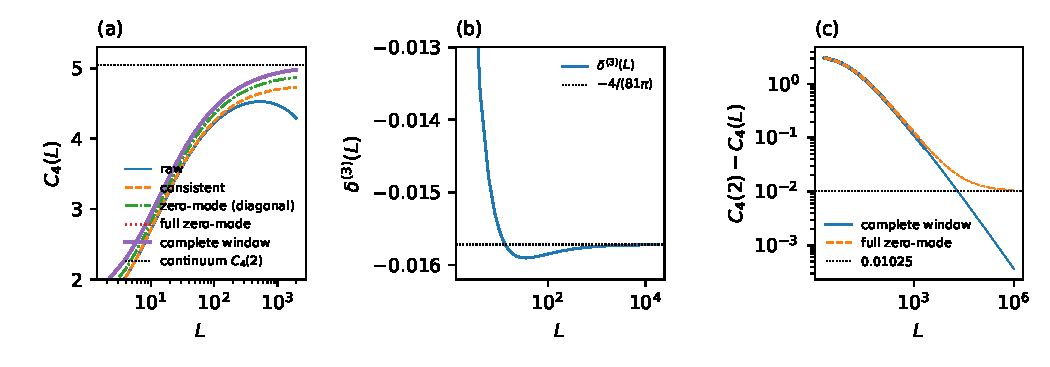
\includegraphics[width=\textwidth]{parts/htp/sections/d2/fig_c4_delta_d2.pdf}
\caption{(a) Exact $C_4(L)$ in $d=2$ for $L\le\HTpTwoLfour$ in five windows: raw, consistent, diagonal zero-mode, full
zero-mode (diagonal and off-diagonal) and complete; only the complete window converges to $C_4^{(2)}$ (dotted). (b) The
$\eps^3$ external-line coefficient $\delta^{(3)}(L)$ of Eq.~\eqref{htp:d2:eq:delta} for $L\le\NTwoDeltaLmax$, with its limit
$-4/(81\pi)$ (dotted); it is not monotone. (c) Distance to the continuum value, $C_4^{(2)}-C_4(L)$, for the complete window
(solid) and the full zero-mode window (dashed); thin lines continue each with its tail fit $T_{22}$ ($300\le L\le2000$,
Appendix~\ref{htp:d2:app:window}). The complete window falls like $\ln^2L/L$; the full zero-mode window levels off at
$0.01025$ (dotted), the part that the mass window $D^M$ supplies. Script \code{make\_fig\_d2.py}.}
\label{htp:d2:fig}
\end{figure}

\subsection{Fifth order}\label{htp:d2:c5}
\emph{All-order window and double counting.} At all orders $D^{\rm zm}$ uses the Bloch matrix of the auxiliary channels
$|z\rangle$ at sub-cutoff $\lambda$, $h(\lambda)=U\,{\rm diag}(E_z(\lambda))\,U^{-1}$ with $U_{z'z}=\langle z'|\psi_z(\lambda)\rangle$, and the mass
window is $D^M=\frac14\{e_1(L)-e_1(L-\hat\ell),M'\}$ with the Newton coefficient $e_1(\lambda)=E_1(\lambda)-E_0(\lambda)$; degenerate partners of $|z\rangle$
($z\ge5$) are projected out. If the auxiliary objects carry their own windows self-consistently, $C_5^W(L)$ diverges linearly,
with coefficient $\NTwoCfiveWLin\pm0.0004$ (the uncertainty of the linear term of raw $C_5$; Table~\ref{htp:d2:tab:c5lin}). The cause is a double counting: a sunset nested in an auxiliary channel is restored once by
the outer $D^M$ and once more inside $h(L-\ell)$. Rule $W_c$ removes it: an auxiliary channel at sub-cutoff $\lambda<L$
represents a zero-mode cluster inside a state of the cutoff-$L$ theory, so its windows are referred to the outer cutoff,
$[h(L)-h(\lambda-\ell_\chi)]$ and $\frac14\{e_1(L)-e_1(\lambda-\hat\ell),M'\}$. It leaves $C_4$ unchanged and removes the linear term (Appendices~\ref{htp:d2:app:Wall} to~\ref{htp:d2:app:tests}).

\emph{External-line window.} In $W_c$ the $\eps^3$ spacing of $\chi_{aa}$ (Sec.~\ref{htp:d2:desc}) tends to a constant,
$R_3\approx\NTwoRthreeWcConst\,a\,w_{aa}$ ($0.062$ to $0.063\,a\,w_{aa}$ at $L=16$ for $a=1$, 2, 3, changing slowly with $L$). An exact test with a tagged external line (Appendix~\ref{htp:d2:app:tag}) locates it: if the external quantum is
invisible to the cutoff and the windows (budget-free), $R_3\to0$; if it is charged its level, $R_3$ reproduces its value
in $W_c$. $D^M$
charges both legs of a mass sub-process with their average level in every slice, which is exact for the $\eps^2$ sunset but not
for the mixed orderings at $\eps^3$. Scheme $W_{cs}$ adds at $\eps^3$
\begin{equation}
 D^{(3)}\mathrel{+}=\frac{\delta^{(3)}(L)}2\,X_0,\qquad \delta^{(3)}(L)=\tfrac14\big[e_1^{(3)}(L-2)-e_1^{{\rm tag},(3)}(L;2,2)\big] ,
 \label{htp:d2:eq:wcs}
\end{equation}
where $X$ is $M'$ with each term multiplied by the summed level of its $\chi$ legs (plus for hops, minus for pair
creation and annihilation), $X_0$ its $\eps^0$ part, and $e_1^{\rm tag}(\lambda;2,2)$ is $E-E_0$ of the $\phi$ channel $|1\rangle$
at cutoff $\lambda$ whose external zero-mode quantum is tagged with charges $(2,2)$: it has level 0 in $H_0$, but the cutoff
and the windows count it as level 2 before it is absorbed and after it is re-emitted (Appendix~\ref{htp:d2:app:wcs}). $\delta^{(3)}(L)$ is an exact rational at each $L$, one number per cutoff; nothing is
fitted (Appendix~\ref{htp:d2:app:wcs} derives the operator form). Chain sums give it for every even $L\le\NTwoDeltaLmax$ (equal to the rationals at $L\le16$ to $\NTwoDeltaRational$).
It is not monotone, with a minimum $\NTwoDeltaMin$ at $L=\NTwoDeltaMinL$ (Fig.~\ref{htp:d2:fig}b), and
\begin{equation}
 \delta^{(3)}(L)=-\frac4{81\pi}-\frac1{54\pi}\,\frac{\ln L}L+\mathcal O(1/L) ,
 \label{htp:d2:eq:delta}
\end{equation}
where the limit $\delta_\infty=-\frac4{81\pi}$ (to $\NTwoDeltaIdent$ by free-limit fits) and the $\ln L/L$ coefficient are
identified numerically, not derived. With this identification the shift $4a\,w_{aa}\delta_\infty=-\frac{16}{81\pi}a\,w_{aa}$
of $R_3(\chi_{aa})$ that the window produces is two thirds of the $\eps^2$ exchange-sunset defect $\frac{8}{27\pi}a\,w_{aa}$
of $R_2$, and $\frac{16}{81\pi}=0.0629$ is close to the $W_c$ remainder above. The shift is therefore expected to cancel
that remainder as $L\to\infty$; this is not established, since $R_3$ is known only to $L=16$. $W_{cs}$ leaves $C_0$ to
$C_4$, $r_{\le3}$ and $g_{\le3}$ unchanged and shifts $C_5$ by $\delta^{(3)}(L)S(L)$, with $S(L)$ the $C_5$ response to
$\frac12X_0$; $S$ has no $\ln L$ and $S_\infty\equiv S(\infty)=\NTwoSinf$, so the shift tends to
$\delta_\infty S_\infty=\NTwoDeltaS$.

\emph{Data and tail} (Appendix~\ref{htp:d2:app:c5tail}). $C_5^{W_{cs}}(L)$ is raw $C_5$ to $L=\HTpTwoLfive$ plus the exact $W_c$ shift and $\delta^{(3)}S$ (both
known to $L=\NTwoShiftLmax$). The tails of $C_2$ to $C_4$ carry $\ln^{n-2}L/L$, and hold-out tests select $\ln^3L/L$ for $C_5$. The
fits use
\begin{equation}
 C_5(L)=A+\sum_{j=0}^{3}a_j\frac{\ln^jL}{L}+\sum_{j=0}^{k_2}a'_j\frac{\ln^jL}{L^2},\qquad k_2\in\{0,1,2\},
 \label{htp:d2:eq:C5tower}
\end{equation}
with no $\ln L$ term, on every even $L$ from $L_{\min}\in\{30,40,60,80,100\}$ to 300. Fitted to $L\le200$, these forms
predict $L=202$ to 300 to $\NTwoBlindNoLog$, against $\NTwoBlindFreeLog$ with a free $\ln L$; fitted to $L\le240$, both
predict $L=242$ to 300 to about $6\times10^{-7}$ (Appendix~\ref{htp:d2:app:c5tail}). The median and half range
of the 15 fits give
\begin{equation}
 C_5=\HTpCfiveTwo\qquad\text{against}\qquad C_5^{(2)}=-38.8336459 ,
 \label{htp:d2:eq:C5}
\end{equation}
with the unrounded median $\NTwoCfiveMedian$, $0.0018$ below the continuum value. Towers with one more power of $\ln L$
at $1/L$ ($k_1=4$), which the hold-out test does not exclude, move the median by only $\NTwoCfiveKfourShift$ but widen the half range
of the fits from $0.013$ to $\NTwoCfiveKfourHalf$ (Appendix~\ref{htp:d2:app:c5tail}); the quoted uncertainty does not include
this. Without the external-line window,
$C_5^{W_c}=\NTwoCfiveWc$ (median $\NTwoCfiveWcMedian$), higher by about $-\delta_\infty S_\infty$ as expected. Both agree
with the continuum value within the spread of the fits, so $C_5$ does not distinguish $W_c$ from $W_{cs}$; the case for
the external-line window rests on the spacing $R_3$ (Sec.~\ref{htp:d2:desc}).

\emph{Residual logarithm.}\label{htp:d2:c5log} A term $b\ln L$ that the data cannot see would move the limit. Over the 15
fits of Eq.~\eqref{htp:d2:eq:C5tower}, the median of the free coefficient drifts from $\NTwoBfreeTwoHundred$ at $L_{\max}=200$
to $\NTwoBfreeThreeHundred$ at 300; a second set of twelve fits ($L_{\min}=30$ to 80) drifts from $-0.0134$ to $+0.0054$
(Appendix~\ref{htp:d2:app:c5tail}). On $C_4^W$, which has no $\ln L$, the 15-fit estimator returns $\NTwoBnull$. On a synthetic
series with a $C_5$-like tail and a known $b$, both sets read about $\NTwoBbias$ low; corrected for this bias, the median
is about $\NTwoBcorr$ (15 fits; $+0.009$ with 12). We take $|b|\lesssim\NTwoBbound$ as a judgement from this median, its
drift and its bias; it is not a confidence bound. The individual fits of the 15-fit set range from $\NTwoBfitMin$ to
$\NTwoBfitMax$, but the extreme ones have nearly as many parameters as points; taken as a bound they would allow shifts of
$C_5$ between about $-0.7$ and $+0.5$. In the 15 fits, fixing $b=\mp\NTwoBbound$ moves the limit by about
$\pm\HTpCfiveTwoLog$, and $b=\NTwoBcorr$ would move it by about $-0.08$; bounding $|b|$ well below $\NTwoBbound$ would
need $L\gtrsim\NTwoLneeded$. The external-line class itself gives no $\ln L$: the
$\ln L$ terms of $S$ cancel within the hop and within the pair sector separately.

\emph{Status.} The complete window has no fitted parameter, removes the $\ln L$ and is verified through $\eps^4$. At $\eps^5$
the rule $W_c$ is needed to remove a linear divergence, and the external-line window to reduce $R_3$ (by at least
$\HTpTwoIdentThree\%$ at $L=14$ and 16). With both, $C_5$ agrees with the continuum. Both rules are provisional: they are
not derived in full, and the window is not proven complete at this order. Like all windows here, they were derived after
their effect had been seen and with the continuum values known.

\subsection{Descendant spacings}\label{htp:d2:desc}
A descendant lies an integer above its primary at every order. With
\begin{equation}
 R_n(L)=\big[E(\chi_{aa})-E(\phi)-2a\big]_{\eps^n},
 \label{htp:d2:eq:R}
\end{equation}
the $\eps^n$ coefficient of the spacing of $\chi_{aa}=\partial^a\bar\partial^a\phi$ computed with the same $r$, $g$ and
window, and the same for the descendants $(\partial\bar\partial)^a\phi^2$ of $\phi^2$, the exact small-$L$ solvers
\code{complete\_exact} and \code{ce\_wc} (Sec.~\ref{htp:d2:solvers}) give every $R_n$, $n\le8$, as rationals for $L\le16$ in each
scheme. These tests need no continuum input; Appendix~\ref{htp:d2:app:legs} gives the data.
\begin{itemize}
\item $\eps^2$: in the consistent and zero-mode windows the exchange sunset of $\chi_{aa}$ has only $L-4a$, and
 $R_2\to\frac{8a\,w_{aa}}{27\pi}$ ($\NTwoRtwoCons$ for $\chi_{11}$ at $L=16$). $D^M$ shifts it by exactly
 $-\frac{8a\,w_{aa}}{27\pi}$, so in the complete window $R_2$ decays like $1/L$ ($\NTwoRtwoWcoef/L$ for $\chi_{11}$), also for
 the $\phi^2$ descendants.
\item $\eps^3$, single-quantum descendants: $R_3(\chi_{11})$ is $\NTwoRthreeWcSixteen$ in $W_c$ and $\NTwoRthreeWcsSixteen$ in
 $W_{cs}$ at $L=16$. At $L=14$ and 16 the window leaves at most 3\% of the $W_c$ value for $a=1$ to 3, so at least
 $\HTpTwoIdentThree\%$ of the defect is removed at $L=14$ and 16. Free-limit fits of $\chi_{11}$ leave a few percent, and the window is
 expected to cancel the defect as $L\to\infty$ (above); $R_3$ itself is not computed beyond
 $L=16$.
\item $\eps^3$, descendants of $\phi^2$: at $L=16$, $R_3=\NTwoPhiDescTwo$ (level 2) and $\NTwoPhiDescFour$ (level 4) in $W_{cs}$;
 the level-4 value still moves away from zero. Not settled.
\item $\eps^4$: in $W_c$ and $W_{cs}$, $R_4(\chi_{11})$ grows, with a local slope of about $\NTwoRfourSlope$ per unit of $\ln L$
 at $L=8$ to 16, while with budget-free legs it goes
 to zero: the same leg defect one order higher. A partial $\chi$-line window ($W_{cs4\chi}$, calibrated on $\chi_{11}$, with the
 $\eps^4$ difference between the $\chi$-line and zero-mode self-energies as a spectator term) closes $\NTwoGapTwo\%$ and
 $\NTwoGapThree\%$ of the gaps of $\chi_{22}$ and $\chi_{33}$ to their budget-free lines at $L=14$, but the $\chi_{22}$ gap is not
 shrinking, the $\phi^2$ descendants still grow, and $R_5(\chi_{aa})$ grows. The window coefficient grows roughly like $\ln L$
 at $L\le16$, which suggests that
 $C_6$ in $W_c$ carries about $\NTwoCsixLog\ln L$ (a prediction, not a measurement). The $\eps^4$ window is not yet known.
\end{itemize}

\subsection{Sixth to eighth order}\label{htp:d2:c6}
$C_6$ to $C_8$ are not reproduced. At $L=16$, $C_6\approx\NTwoCsixSixteen$ in $W_c$, $W_{cs}$ and $W_{cs4\chi}$
(Table~\ref{htp:d2:tab:c6}), $54\%$ below the continuum value $\NTwoCsixCont$, and $C_6(L)$ still rises by about
$\NTwoCsixStep$ per step of 2 in $L$. The external-line windows shift $C_6$ by about $10^{-4}$ of its value there, while
$W$ and $W_c$ differ by about 1\% (Appendix~\ref{htp:d2:app:c6eps5}). The production tables to $L=\HTpTwoLprod$ (raw and
consistent) are shipped as finite-cutoff data, but those windows diverge from $\eps^4$ on, and the external-line windows
from $\eps^4$ on are not known.
}{\section{Results in two dimensions}\label{htp:d2:sec}(Contribution of HT2dPert pending.)}
\IfFileExists{parts/htp/sections/d3/sec_d3.tex}{% sec_d3.tex (HT3dPert, 2026-10-14, second version; edited by HT1dPert 2026-10-15 for the note review, facts from
% HT3dPert): d = 3 perturbative HT. Numbers: numbers_d3.tex; table tab_d3_coeffs.tex (code/lri_3d_hpc/public/note_d3.py);
% figure fig_d3_c4.pdf (code/lri_3d_c4_exact/public/note_fig_d3.py); reproduction rows: repro_d3.tex; package rows:
% packages_d3.tex; checks and caveats: checks_d3.tex, caveats_d3.tex.
\section{Results in three dimensions}\label{htp:d3:sec}

\paragraph{Model and cutoff.}
In $d=3$ the generalized free field is quantized on $S^2$ (Sec.~\ref{htp:sec:method}, Ref.~\cite{htp:Hogervorst:2014rta}). A
mode $(n,\ell,m)$ has energy $\Ds+2n+\ell$, with $\ell$ the angular momentum; the zero mode $n=\ell=0$ is the local
oscillator, and all other modes form the bath. We keep the states with bath level
\begin{equation}
 N_b=\sum_{(n,\ell,m)\neq(0,0,0)}(2n+\ell)\,n_{n\ell m}\le L
 \label{htp:d3:eq:cutoff}
\end{equation}
and do not truncate the zero mode. The perturbation is $H=H_0+r\,M+g\,V$ with
$M=\int d\Omega\,{:}\phi^2{:}/(4\pi)$ and $V=\int d\Omega\,{:}\phi^4{:}/(48\pi)$. $r$ and $g$ are tuned order by order
to $E_1-E_0=\Ds$ and $E_3-E_0=3-\Ds$, and
\begin{equation}
 \DE(\eps;L)=E_2-E_0=\tfrac32-\tfrac{\eps}{6}+\sum_{n\ge2}C_n(L)\,\eps^n,\qquad \Ds=\frac{3-\eps}{4}.
 \label{htp:d3:eq:Cn}
\end{equation}
The continuum values $C_n^{(3)}$ are those of Table~\ref{htp:tab:refvals}.

\paragraph{Two codes.}
The production package (\code{code/lri\_3d\_hpc/}) builds the truncated Hamiltonian explicitly in the SO(3)-scalar,
inversion-even sector and solves the Rayleigh--Schr\"odinger recursion through $\eps^8$ in x87 long double. It reached
$L=16$, 18 and \HTpThreeLmax{} (\NThreeScalarTwenty{} scalar bath states at $L=20$, from \NThreeStatesTwenty{} before
the projection; about \NThreeSU{} service units on SDSC Expanse, charge units of about one per core-hour, with
large-memory jobs charged more). It implements two prescriptions: raw, and the vacuum window
$D_L(N_b)=E_v(L)-E_v(L-N_b)$.

The exact-sum package (\code{code/lri\_3d\_c4\_exact/}) evaluates the same coefficients as sums over intermediate states,
with exact partial-wave reductions on $S^2$ and exact zero-mode projections, at every even $L$:
\begin{itemize}
\item $C_2$ to $L=\HTpThreeLwin$, $C_3$ and $C_4$ to $L=\HTpThreeLfour$, $C_5$ to $L=\HTpThreeLfive$;
\item every window shift to $L=\HTpThreeLwin$;
\item every window scheme, including the complete window of $d=2$ (Sec.~\ref{htp:d2:sec}).
\end{itemize}
At every even $L\le20$ the two codes agree on $C_2$ to $C_5$, $r$, $g$ and the reference energies $E_0$ to $E_3$ to
$\NThreeValPkg$. The window schemes that the production package lacks agree with a brute force, built as explicit
operators on the package's own Hamiltonian at $L\le14$, to $\NThreeValBrute$. Table~\ref{htp:d3:tab:coeffs} gives the
production values.

% tab_d3_coeffs.tex: generated by code/lri_3d_hpc/public/note_d3.py from data/HT_3d/pert3d/results (do not edit)
\begin{table}[ht]\centering\footnotesize\setlength{\tabcolsep}{3pt}
\begin{tabular}{@{}l lll lll@{}}\toprule
 & \multicolumn{3}{c}{consistent (vacuum window $D_L$)} & \multicolumn{3}{c}{raw}\\
\cmidrule(lr){2-4}\cmidrule(lr){5-7}
 & $L=16$ & $L=18$ & $L=20$ & $L=16$ & $L=18$ & $L=20$\\\midrule
$C_2$ & 0.1799805130 & 0.1801641045 & 0.1803065210 & 0.1799805130 & 0.1801641045 & 0.1803065210\\
$C_3$ & $-$0.3238079917 & $-$0.3271370505 & $-$0.3298433574 & $-$0.3238079917 & $-$0.3271370505 & $-$0.3298433574\\
$C_4$ & 0.7154707349 & 0.7295143865 & 0.7400078407 & 0.7082381633 & 0.7206323697 & 0.7293066716\\
$C_5$ & $-$3.157412985 & $-$3.274129748 & $-$3.376315158 & $-$3.173233312 & $-$3.292870751 & $-$3.398184422\\
$C_6$ & 15.68169942 & 16.38726028 & 17.03798989 & 15.67552153 & 16.38079206 & 17.03198660\\
$C_7$ & $-$84.42870757 & $-$88.02482107 & $-$91.14377531 & $-$84.17501495 & $-$87.66743530 & $-$90.65688526\\
$C_8$ & 548.2872011 & 578.4398685 & 605.8501134 & 548.2146549 & 578.3577582 & 605.7652262\\
\bottomrule\end{tabular}
\caption{Finite-cutoff coefficients $C_n(L)$ in $d=3$ from the production package \code{lri\_3d\_hpc} (10 significant digits; the records hold 20), raw and with the vacuum window $D_L$. $C_2$ and $C_3$ do not depend on the window. The exact sums reproduce $C_2$ to $C_5$ of this table to $3\times10^{-13}$; from $C_4$ on, neither scheme converges (Fig.~\ref{htp:d3:fig:c4}).}
\label{htp:d3:tab:coeffs}\end{table}


\paragraph{The vacuum window diverges at $\eps^4$.}
$C_2(L)$ and $C_3(L)$ do not depend on the window and converge. From $C_4$ on, the vacuum window does not suffice
(Fig.~\ref{htp:d3:fig:c4}).
\begin{itemize}
\item As in $d=2$, divergent sub-bubbles inside a state see only the level left by the other quanta, while $r$, $g$ and
 the vacuum are tuned with the full $L$.
\item In $d=3$ the mass sub-bubble diverges like $L^{3/2}$ instead of $L$, so every term is one power worse.
\item Uncorrected, $C_4(L)$ falls like $-\NThreeRawLsq\,L^2$.
\item With $D_L$ alone it peaks at $\NThreeCfourConsPeak$ near $L=32$ and is $\NThreeCfourConsSix$ at $L=600$. The
 terms are $-\NThreeConsLin\,L$ and $-\tfrac{10}{243\,\Gamma(7/2)}\sqrt L\ln L$, which the diagonal and
 zero-mode-number-changing parts of the zero-mode window remove.
\item The mass window ($\chi$-attached sunset term), which in $d=2$ is a finite shift, here removes a further
 $\NThreeChiSqrt\sqrt L$.
\end{itemize}

\paragraph{Complete window.}
The complete window $W$ of $d=2$ is carried over unchanged: vacuum window, full zero-mode window, and mass window
$-\tfrac12 r_2'(L)\{\hat N_b,M'\}$, with $\hat N_b$ the bath-level operator. With it, $C_4(L)$ converges like $1/L$. At
$L=600$ it is $\NThreeCfourWsix$. With the limit fixed at $C_4^{(3)}$, a free $\sqrt L$ term comes out below
$\NThreeNoDiv$. The mass window is used in its leading-order linear form; since $r_2$ is not linear in $L$ in $d=3$, the
exact form may differ by a finite amount, which the agreement below suggests is small but which is not derived.

At $\eps^5$ the nested windows are referred to the outer cutoff (rule $W_c$ of $d=2$); the external-line window
($W_{cs}$) changes $C_5(40)$ by $-0.003$.

\begin{figure}[ht]\centering
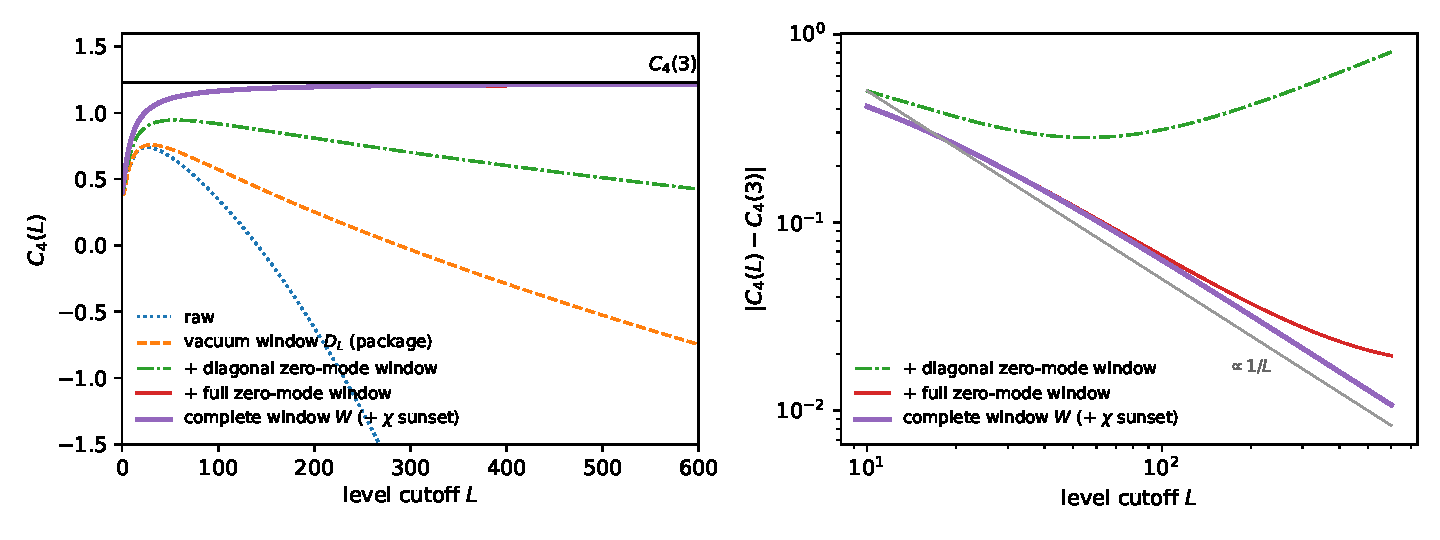
\includegraphics[width=\linewidth]{parts/htp/sections/d3/fig_d3_c4.pdf}
\caption{$C_4(L)$ in $d=3$ from the exact sums, in each window scheme. Left: raw, the vacuum window $D_L$ of the
production package, and the zero-mode and mass windows added one by one (the full-zero-mode curve lies under $W$ at this
scale). Right: distance from $C_4^{(3)}$ on logarithmic axes. The complete window $W$ converges like $1/L$; without its
mass window the distance stops decreasing, has its minimum near $L\approx1100$ and grows like $3.6\times10^{-4}\sqrt L$
beyond the plotted range.}
\label{htp:d3:fig:c4}
\end{figure}

\paragraph{Extrapolations.}
Fit forms (towers of $L^{-k}\ln^jL$ terms, from the $d=2$ protocol) and windows were chosen after the data were seen,
with the continuum values known; the quoted uncertainties are spreads over fits, not standard errors.
\begin{itemize}
\item $C_2=\HTpCtwoThree$ ($\HTpCtwoThreeDigits$ digits of the closed form; fit to $L\le\HTpThreeLwin$).
\item $C_3=\HTpCthreeThree$ ($\delta=\HTpCthreeThreeDev$): mean and half-range of three fit windows.
\item $C_4=\HTpCfourThree$ ($\delta=\HTpCfourThreeDev$): median of one tower over 12 fit windows; the uncertainty is
 the half-range, including a blind fit to $L\le400$ that predicts $402\le L\le600$ to $\NThreeCfourBlind$. Towers with
 one more correction term spread to about $10^{-4}$.
\item $C_5$, provisional and calibrated on $C_4^{(3)}$: towers are kept if, on $C_4^W(L)$ at the same $L\le40$, they
 reproduce $C_4^{(3)}$ to within 0.036 and pass a blind test. The median of their $C_5$ fits gives $\HTpCfiveThree$
 (median $\NThreeCfiveMed$) against $C_5^{(3)}=-5.850351421$. The uncertainty is the worst $C_4$ miss relative to the
 remaining $C_4$ correction at $L=40$ (0.036 of 0.147), times the remaining $C_5$ correction at $L=40$ (1.28, which
 uses $C_5^{(3)}$ itself).
 \begin{itemize}
 \item This is a weak test: $C_5^{W_c}(40)=\NThreeCfiveWcForty$ is still 1.28 above the limit.
 \item A term in $L^{-1/2}$, which $L\le40$ cannot exclude, would lower the limit by 0.5 to 1.
 \item A window without the mass window also fits at $L\le40$, although it differs from $W_c$ by a term growing like
  $L^2$.
 \item Going further needs a new representation of the angular channels: the cost grows like $L^{8.4}$ and the memory
  like $L^{4.5}$.
 \end{itemize}
\end{itemize}

\paragraph{Descendant spacings.}
For the scalar descendant of $\phi$ (the $n=1$, $\ell=0$ quantum), the window removes the $\eps^2$ violation of its
spacing as $L\to\infty$. At $\eps^3$ the external-line window acts in the right direction, but the violation is not shown
to vanish at $L\le16$.
}{\section{Results in three dimensions}\label{htp:d3:sec}(Contribution of HT3dPert pending.)}
% s06_checks.tex (HT1dPert): independent checks; d = 2, 3 paragraphs are \input from their folders.
\section{Independent checks}\label{htp:sec:checks}

\paragraph{One dimension.}
\begin{itemize}
\item \emph{Window engines.} The complete window through $\eps^5$ was computed by two independent engines, one on the
 solver's kernels and one written from scratch with exact rationals, plus a third engine for a skeptic's check. Four
 algorithms within the second engine agree to $1.3\times10^{-11}$; the two engines agree on 3808 numbers to
 $9.6\times10^{-12}$; the third reproduces $\Delta C_5$ at $\Lambda\le28$ to $2.4\times10^{-12}$
 (quoted as $\HTpEngineAgree$ in the paper).
\item \emph{Eighth-order window.} The complete-window solver reproduces the exact $\Delta C_4$, $\Delta C_5$ at
 $\Lambda=46$--$72$ to $\HTpSTenMatch$.
\item \emph{Exact sums against the solver.} The exact sums reproduce the solver's raw $C_4$ and $C_5$ at
 $\Lambda\le118$ to $1.4\times10^{-12}$ and $10^{-11}$, and the window pieces to $10^{-15}$; brute-force
 Rayleigh--Schr\"odinger on explicit bases at small cutoffs agrees to $10^{-11}$.
\item \emph{Eighth-order code.} The optimized eighth-order code reproduces the 38 saved records of its original
 version to $2.1\times10^{-8}$ and the thermal solver's $C_0$--$C_7$ to $6\times10^{-14}$ relative.
\item \emph{Blind protocol of the exact sums.} Fit records were frozen and hash-committed before each larger run
 existed: $\Lambda\le1000$ before $2000$ for $C_4$, $\Lambda\le320$ before 400 and $\Lambda\le400$ before 500 for $C_5$.
 Their predictions of the new cutoffs are quoted in Section~\ref{htp:d1:sec:extrap}.
\item \emph{Constrained $C_5$.} A separately written fit of the constrained extrapolation, made without reading the
 package's fit code, gives $\HTpCfiveOne$; a separate derivation confirms $\omega_1=\tfrac72$ as the one-loop
 exponent of $\phi^6$ and the closed form \eqref{htp:eq:toplog}.
\end{itemize}
\IfFileExists{parts/htp/sections/d2/checks_d2.tex}{% checks_d2.tex -- d = 2 paragraph of the independent-checks section (from HT2dPert, 2026-10-14). Checks p2.*.
\paragraph{Two dimensions.}\label{htp:d2:checks}
Two solvers were written from a first-principles specification of the $d=2$ model (Sec.~\ref{htp:d2:model}) by agents that saw
neither the production code nor each other's work. The first is plain Rayleigh--Schr\"odinger perturbation theory to $\eps^8$
with full wavefunction corrections in exact rational arithmetic, in two codes (\texttt{fractions} over the full space, and a
reflection-reduced code modulo many primes with rational reconstruction checked on held-out primes), for
$L=0,\dots,\NTwoRSLmax$ in all three schemes. The second uses no perturbation theory: the truncated Hamiltonian is built at
complex $\eps$ on a circle with 256-bit arithmetic, $r$ and $g$ are Newton-solved, the eigenvalues are followed from the
references, and Cauchy integrals give the coefficients, for $L\le\NTwoCauchyLmax$. Over $C_n$, $r_n$, $g_n$, the reference
energies and all sub-cutoff vacua, $n\le8$, the production solver agrees with the exact one to $\HTpTwoImplAgree$ (scaled
difference $\max|a-b|/\max(1,|b|)$; raw and consistent $L\le\NTwoRSLmax$, literal $L\le14$), the Cauchy solver with the exact one
to $\NTwoCauchyAgree$, and the production $C_n$ with the Cauchy ones to $\NTwoPkgCauchy$. The large-$L$ sum codes of
Sec.~\ref{htp:d2:solvers} reproduce these values at small $L$. The raw scheme was specified from first principles; for the
consistent and literal schemes the definitions were taken from the production package, so there the check covers the
implementation, not the choice of window. These checks verify that we compute the stated truncation; they do not test its
continuum limit.
}{}
\IfFileExists{parts/htp/sections/d3/checks_d3.tex}{% checks_d3.tex: d = 3 paragraph of the independent-checks section (moved from sec_d3.tex by HT1dPert, 2026-10-15,
% facts from HT3dPert).
\paragraph{Three dimensions.}\label{htp:d3:checks}
These checks show that the codes compute the stated truncation; the windows and fit forms are the assumptions.
\begin{itemize}
\item \emph{Two codes:} the exact sums and the production package agree to $\NThreeValPkg$ at $L\le20$
 (Sec.~\ref{htp:d3:sec}).
\item \emph{Original implementation:} the precomputed Hamiltonian of each production cutoff, solved at
 $L=\HTpThreeGateL$, agrees with the original implementation shipped in the package to $\NThreeGateMax$.
\item \emph{Stored Hamiltonians:} the one of $L=20$ reproduces those of $L=16$ and $L=18$ to $\NThreeCrossStore$.
\item \emph{Recursion:} every recursion residual is at most $\NThreeResid$.
\item \emph{Engine regression:} the final $\eps^5$ engine reproduces the stored $L\le20$ run to $5\times10^{-13}$ and all
 reduced $L=40$ sub-sums bit for bit.
\end{itemize}
}{}

% s07_caveats.tex (HT1dPert); d = 2, 3 paragraphs are \input from their folders.
\section{Caveats}\label{htp:sec:caveats}

\paragraph{One dimension.}
\begin{itemize}
\item The windows were derived after their effects had been seen and with the continuum values known, though with no
 fitted parameter.
\item The extrapolation dominates the error, and the exponents \eqref{htp:eq:omega} are an assumption. Fits that reach the
 exact $C_5$ need an effective $\omega_3$ of $\HTpOmegaThreeEff$, not the gap value $\HTpOmegaThree$. A second channel
 with the leading power $\Lambda^{-1/2}$, from the phase operator of the cutoff kernel, enters at $\eps^4$ (cited check
 \code{code/lri\_d1\_fullblock\_tail\_response}); it does not affect the top logarithm \eqref{htp:eq:toplog} but does affect
 the lower ones, so tying them to $\omega_2$, $\omega_3$ is not exact.
\item The $\eps^4$ top-log coefficient fitted from the exact $C_4(\Lambda)$ lies $\NOneTopLogFour$ from
 Eq.~\eqref{htp:eq:toplog}, depending on the basis; whether this is a real violation is undecided. Taking $c_5$ from the
 $C_2$ chain of Eq.~\eqref{htp:eq:toplog} instead, a value $0.3\%$ smaller, moves the constrained $C_5$ by $4\times10^{-4}$ to
 $1.4\times10^{-3}$ (absolute), far below its quoted uncertainty (\code{xchk/REPORT\_blind.md} of \code{lri\_1d\_c5\_exact}).
\item A test protocol for the raw $C_4$ and $C_5$, fixed before most of the large-cutoff data had been seen, had mixed
 results: its held-out predictions passed; window stability failed for $C_5$ in two of three bases and for $C_4$ in one,
 and tail insensitivity failed for $C_5$. Every $d=1$ fit beyond $C_3$ involves choices made after the data were seen, apart from the blind
 predictions of the exact sums. The constrained $C_5$ fit's selection thresholds were set after a run had printed the
 exact value; the separately written fit is the quoted determination.
\item $C_8$, calibrated on the diagrammatic $C_6$ and $C_7$, is not an independent determination.
\item We have not constructed an effective Hamiltonian beyond the windows.
\end{itemize}
\IfFileExists{parts/htp/sections/d2/caveats_d2.tex}{% caveats_d2.tex -- d = 2 caveats (from HT2dPert, 2026-10-14).
\paragraph{Two dimensions.}\label{htp:d2:caveats}
The windows of Secs.~\ref{htp:d2:c4} and \ref{htp:d2:c5} were derived after their effects had been seen and with the continuum values
known, though they contain no fitted parameter. The complete window is verified through $\eps^4$; at $\eps^5$ the rule $W_c$
and the external-line window are needed as well, and the window is neither derived in full nor proven complete there. The limit
$-4/(81\pi)$ of $\delta^{(3)}$ is identified numerically. The quoted limits are spreads over tail models and fit windows, not
standard errors. The $C_5$ value assumes no residual $\ln L$ term; one with $|b|\lesssim\NTwoBbound$, a bound judged from the
median of the fits rather than a confidence bound, is not excluded at $L\le\HTpTwoLfive$ and would move $C_5$ by up to about
$\HTpCfiveTwoLog$. $C_5$ does not distinguish $W_c$ from $W_{cs}$; the external-line window rests on the spacing $R_3$. The $\eps^3$ spacings of the $\phi^2$ descendants are not settled at $L\le16$, the $\eps^4$
window is not known, and $C_6$ to $C_8$ are not reproduced. The production tables (raw and consistent schemes) diverge from
$\eps^4$ on, linearly in $L$ (raw) and like $\ln L$ (consistent), so they are finite-cutoff data of those schemes, not continuum
estimates.
}{}
\IfFileExists{parts/htp/sections/d3/caveats_d3.tex}{% caveats_d3.tex: d = 3 caveats (HT1dPert, 2026-10-15, facts from HT3dPert).
\paragraph{Three dimensions.}\label{htp:d3:caveats}
The fit forms and windows were chosen after the data were seen, with the continuum values known. The mass window is used
in its leading-order linear form, which is not derived for $d=3$. The $C_4$ uncertainty is the spread of one tower over
12 fit windows; towers with one more correction term spread to about $10^{-4}$. $C_5$ is provisional: it is calibrated on
$C_4^{(3)}$, the scale of its uncertainty uses $C_5^{(3)}$ itself, a term in $L^{-1/2}$ is not excluded at $L\le40$, and
at $L\le40$ the test cannot separate $W_c$ from the window without the mass window. The $\eps^3$ violation of the descendant
spacing (scalar descendant of $\phi$) is not shown to vanish at $L\le16$. The last digit of $C_3$ is platform-sensitive: one fit window moves by about
$10^{-9}$ between machines, and the replay checks it to a tenth of the stated uncertainty.
}{}

% s08_repro.tex (HT1dPert): reproduction section; rows come from repro_d1.tex, sections/d2/repro_d2.tex, sections/d3/repro_d3.tex
\section{Reproduction}\label{htp:sec:repro}

\subsection{Layout}
All paths are relative to the folder \code{HT\_Pert/} of the public repository.
\begin{itemize}
\item \code{code/<package>/}: one package per solver or analysis, shipped at the commit its production ran. Each has a
 \code{public.mk} with the targets \code{test} and \code{replay} (some also \code{smoke}, \code{replay-full},
 \code{fetch-data}) and a \code{public/} folder with the replay scripts.
\item \code{data/HT\_<d>d/}: the production records.
\item \code{results/HT\_<d>d/}: the expected value of every quoted number (\code{quoted\_numbers.json}) and summaries.
\end{itemize}
\code{make test} and \code{make replay} in \code{HT\_Pert/} run the targets of every package; in a package folder,
\code{make -f public.mk test|replay}. A replay recomputes every quoted number of its package from the shipped records,
without a production rerun, prints a PASS/FAIL table and exits non-zero on any failure.

\subsection{Packages and records}
\begingroup\footnotesize\renewcommand{\arraystretch}{1.15}
\begin{longtable}{@{}p{4.4cm}p{2.3cm}p{8.2cm}@{}}
\toprule
package (\code{code/}) & $d$, role & content, records, cost\\
\midrule\endhead
\bottomrule\endfoot
\code{lri\_hpc\_Hamitonian} & 1: solver, analyses & HT solver to $\eps^7$; joint tail fits, window engines, identities. Records \code{data/HT\_1d/thermal\_expanse} (111 cutoffs) and the analysis outputs \\
\code{lri\_eh\_hpc} & 1: window & isolated $g^2D$ window, closed form $K$ \\
\code{lri\_c8\_hpc} & 1: solver & eighth order, $\Lambda\le\HTpLamCeight$; records \code{data/HT\_1d/c8} \\
\code{lri\_d1\_full\_coefficient\_flow} & 1: solver & complete window through $\eps^8$, $\Lambda\le\HTpWinLamEight$; records \code{data/HT\_1d/s10\_production} \\
\code{lri\_1d\_dconn\_refit} & 1: analysis & extrapolations of $C_4$--$C_8$ with the complete window \\
\code{lri\_1d\_c4\_exact}, \code{lri\_1d\_c5\_exact} & 1: exact sums & $C_2$--$C_4$ to $\Lambda=\HTpOneLexact$, $C_5$ to $\NOneCfiveLmax$; records \code{data/HT\_1d/exact\_c4}, \code{exact\_c5}; blind fit records \\
\code{lri\_d1\_fullblock\_tail\_response} & 1: cited check & second $\Lambda^{-1/2}$ channel \\
\IfFileExists{parts/htp/sections/d2/packages_d2.tex}{\inputrows{parts/htp/sections/d2/packages_d2.tex}}{}
\IfFileExists{parts/htp/sections/d3/packages_d3.tex}{\inputrows{parts/htp/sections/d3/packages_d3.tex}}{}
\end{longtable}
\endgroup

\subsection{Rules that are part of the results}
The fit families and windows, the selection and calibration rules, the rounding of quoted ranges and the status words
are part of the results; the \code{REPRODUCE} file of each package lists them under ``Decisions you must not make''.

\subsection{\texorpdfstring{Result $\to$ code, record, command, tolerance}{Result to code, record, command, tolerance}}
\begingroup\footnotesize\renewcommand{\arraystretch}{1.15}
\begin{longtable}{@{}>{\raggedright}p{3.7cm}>{\raggedright}p{2.8cm}p{0.8cm}>{\raggedright}p{2.75cm}>{\raggedright}p{2.25cm}>{\raggedright\arraybackslash}p{1.6cm}@{}}
\toprule
result & value & pkg & records & command & tolerance\\
\midrule\endhead
\bottomrule\endfoot
\inputrows{parts/htp/sections/repro_d1.tex}
\midrule
\inputrows{parts/htp/sections/d2/repro_d2.tex}
\midrule
\inputrows{parts/htp/sections/d3/repro_d3.tex}
\end{longtable}
\endgroup

\appendix
% app_d2_eps4.tex -- d = 2 appendix, part 1 of 3 (HT2dPert, 2026-10-16): operators and schemes at low order, solver
% checks, exact C4(L), the mechanism of the ln L divergence class by class, and the complete window at eps^4.
% Merged from the method write-up of package I (public edition of 2026-10-14), which these appendices
% replace; superseded material is not carried over, and what Sec. d2:sec states is not repeated.
% Notation of Sec. d2:sec and Table tab:notation (level l, operator \hat l, sub-cutoff lambda, e_1 = E_1 - E_0).
% Numbers quoted in Sec. d2:sec use the macros of numbers_d2.tex (replay rows in repro_d2.tex); every other number is
% read from, or (where marked) evaluated from, the records named in the subsection (all shipped in package I).
\section{Two dimensions: operators, exact fourth order and the complete window}\label{htp:d2:app:eps4}

Appendices~\ref{htp:d2:app:eps4} to~\ref{htp:d2:app:legs} give the derivations and the supporting data behind
Section~\ref{htp:d2:sec}. This appendix covers the operators and schemes at low order, the solver checks, the exact $C_4(L)$,
the cause of its $\ln L$ divergence class by class, and the complete window at $\eps^4$. Appendix~\ref{htp:d2:app:eps5}
treats order $\eps^5$: the window at all orders, the double counting that rule $W_c$ removes, and the tail of $C_5$.
Appendix~\ref{htp:d2:app:legs} treats the descendant spacings and the external-line windows $W_{cs}$ and $W_{cs4\chi}$, and
ends with the status of each window component. Paths are relative to the package
\code{code/\allowbreak{}lri\_2d\_coeff\_independent\_check/} (package I of Section~\ref{htp:sec:repro}), and each subsection names its
records. Numbers that Section~\ref{htp:d2:sec} also quotes have reproduction rows in Section~\ref{htp:sec:repro}. The other numbers
of these appendices are read from the records named in each subsection, or evaluated from them where the text says
so; the reproduction scripts do not recompute them. ``Exact'' data
are rationals, or float64 evaluations of exact finite sums with a measured rounding error of at most
$1.4\times10^{-11}$. Limits $L\to\infty$ are fits; their uncertainties are spreads over tail models and fit windows, not
standard deviations.

\subsection{Operators and schemes at low order}\label{htp:d2:app:ops}
{\small\raggedright\noindent Records: \code{SPEC.md}, \code{rs\_exact/\allowbreak{}README.md}, \code{zeromode\_exact/\allowbreak{}README.md},
\code{cauchy/\allowbreak{}README.md}.\par}

\paragraph{Factorized vertices.} With $Z=a_0+a_0^\dagger$, $a_0=A_{00}$, and $\chi=\phi-Z$, normal ordering factorizes:
\begin{equation}
 V=\sum_{m=0}^4\frac1{12}\binom4m{:}Z^{4-m}{:}\otimes\langle{:}\chi^m{:}\rangle_\theta,\qquad
 M=\sum_{m=0}^2\binom2m{:}Z^{2-m}{:}\otimes\langle{:}\chi^m{:}\rangle_\theta .
 \label{htp:d2:eq:factorize}
\end{equation}
At $\eps=0$ the weights factorize holomorphically, $w_{ab}=v(a)v(b)$ with $v(a)=(\frac12)_a/a!$. The squared
$V$-vertex coefficient times the Wick count of a bundle of $m$ $\chi$ lines is
$\gamma_m=m!\,\big[\binom4m/12\big]^2$: $\gamma_1=\frac19$, $\gamma_2=\frac12$, $\gamma_3=\frac23$, $\gamma_4=\frac16$.

\paragraph{Space and particle cap.} The truncated space holds the occupation states with spin zero, even under
$(a,b)\to(b,a)$, and $\ell\le L$; spin zero forces $\ell$ even, and the field parity $(-1)^P$ is conserved. Truncated
operators are the projections of the full ones; nothing else is truncated. The level cutoff does not bound $P$, because
zero-mode quanta cost no level. A path argument shows that a contribution to the order-$\eps^n$ energy of $|p\rangle$
reaches at most $P=p+4\lfloor n/2\rfloor$, which gives the cap $P\le p+16$ through $\eps^8$. It was also tested: caps
$p+18$ and $p+20$ reproduce the $p+16$ rationals identically, while $p+14$ changes $C_8$ and nothing below. The Cauchy
code confirms it with absolute caps: $P\le21$ and $P\le23$ reproduce $P\le19$, and $P\le17$, 18 change only $C_8$.

\paragraph{References and the projection $\Pi$.} Each reference $|p\rangle$ is non-degenerate in its sector, so $E_p(\eps)$
is unique. Because $w_{00}=1$ and every window has vanishing diagonal elements on level-0 states, $\langle p|M|p\rangle=2p$ and
$\langle p|V|p\rangle=\frac12p(p-1)$ at every $\eps$. With $\mathcal E_p^{(n)}$ the order-$n$ energy without the $r_n$,
$g_n$ terms, Eq.~\eqref{htp:eq:Pi} reads $C_n=\Pi[\mathcal E^{(n)}]$ with
\begin{equation}
 \Pi f=f(2)-f(1)-\tfrac13\big[f(3)-f(0)\big]=-\tfrac13\Delta^3f(0),\qquad \Pi[p^3]=-2,\qquad \Pi[p^4]=-12 ,
 \label{htp:d2:eq:Pi}
\end{equation}
and $\Pi$ annihilates every polynomial of degree at most two in $p$. Only the part of an energy shift that is at least
cubic in $p$ reaches $C_n$.

\paragraph{Where the schemes differ.} The diagonal windows (consistent, literal, zero-mode) are of order $\eps^2$ and
vanish on $|p\rangle$, so they first enter through $\langle p|H_1G_pD_2G_pH_1|p\rangle$ at $\eps^4$, with $H_1=F_1+g_1V$ and the resolvent
$G_p=Q_p/(\frac p2-H_0)$, $Q_p$ the projection off $|p\rangle$. Raw and consistent therefore differ first at $C_4$. Raw
and consistent vacua agree through $\eps^3$, so the consistent and literal windows differ first at $C_6$; the exact data
confirm both statements for every $L>0$. At $\eps^4$ only the $\eps^2$ parts of the windows matter:
\begin{equation}
 D^{\rm cons}_2(\ell)=E_v^{(2)}(L)-E_v^{(2)}(L-\ell),\qquad
 E_v^{(2)}(\lambda)=g_1^2\langle0|VG_0V|0\rangle_\lambda=-\frac{(\lambda+2)(\lambda+4)}{864},
 \label{htp:d2:eq:Ev2}
\end{equation}
where $\langle\cdot\rangle_\lambda$ restricts the intermediate states to level $\le\lambda$, and the zero-mode window is
$D_2^{\rm zm}(z,\ell)=h^{(2)}_{zz}(L)-h^{(2)}_{zz}(L-\ell)$, the diagonal of Eq.~\eqref{htp:d2:eq:Dzm}. The $r_2$ and $g_2$ terms of
the sub-cutoff energies cancel in these differences, and for $z=0$ the two windows coincide.

\paragraph{Degenerate partners.} For $z\ge5$ the zero-mode channel $|z\rangle$ has degenerate partners with level
$\ell=2,4,\dots\le\frac{z-1}2$ and $P=z-2\ell$. First order lifts the degeneracy (smallest separation $\frac73$, at $z=5$,
$\ell=2$), so the branch through $|z\rangle$ is unique; the references are never degenerate. The window objects project
the partners out (Appendix~\ref{htp:d2:app:Wall}).

\subsection{Solver checks in detail}\label{htp:d2:app:checks}
{\small\raggedright\noindent Records: \code{compare\_with\_package.txt}, \code{compare\_three\_way.txt}, \code{rs\_exact/\allowbreak{}README.md},
\code{cauchy/\allowbreak{}README.md}, the production records \code{../\allowbreak{}../\allowbreak{}data/\allowbreak{}HT\_2d/\allowbreak{}prod/}, \code{continuum/\allowbreak{}exact\_C2\_C3.csv}, \code{continuum/\allowbreak{}asymptotics\_C2\_C3.txt}; code
\code{continuum/\allowbreak{}exact\_low\_orders.py}.\par}

\paragraph{The three computations.} Section~\ref{htp:d2:solvers} and the independent-checks paragraph of
Section~\ref{htp:sec:checks} give their scope and agreement. The production solver propagates Taylor jets of the wave
functions in float64, with scalar reductions in extended long double; its consistent run at $L=34$ took 2893\,s on 64
threads with a peak memory of 463\,GiB. The exact solver works in a similarity frame in which every matrix element is
rational; its modular code uses 72 primes with Chinese remaindering, and every rational reconstruction is verified on
eight held-out primes. The Cauchy solver evaluates $\DE$ at $\eps_k=\rho\,e^{2\pi\mathrm ik/K}$ with $\rho=\frac1{64}$,
$K=128$ and 256-bit arithmetic, and $C_n=K^{-1}\sum_k\DE(\eps_k)\eps_k^{-n}$. It solves the consistent vacua exactly. On states with
$\ell\ge2$ the window is $E_v(\lambda)-E_v(\lambda-\ell)$, so the self-consistent condition $(H_\lambda+D_\lambda)\psi=E_v(\lambda)\psi$
becomes the linear generalized eigenproblem $A_\lambda\psi=E_v(\lambda)\,\mathcal P_0\psi$, with
$A_\lambda=H_\lambda-E_v(\lambda-\hat\ell)(1-\mathcal P_0)$, $\mathcal P_0$ the projection on level-0 states, and the
sub-cutoff vacua $E_v(\lambda-\ell)$ known from smaller $\lambda$.

\paragraph{Internal checks of the exact codes.}
\begin{itemize}
\item $C_0=1$, $C_1=-\frac16$, $r_1=0$, $g_1=\frac13$ for every $L$ and scheme, and the tuning conditions hold exactly at
 every order. The fraction and modular codes agree identically for every number at $L\le12$.
\item A third, Hermitian construction of $H$ was diagonalized at 110 digits at $\eps=10^{-3}$, $10^{-5}$, $10^{-8}$, with the
 exact series for $r$, $g$ and the vacua inserted ($L\le6$, every scheme and channel). The residual divided by $\eps^9$
 tends to a constant, which confirms every coefficient through $\eps^8$ to about $10^{-8}$.
\item The Cauchy results do not change with the circle radius, the number of points, the precision, the continuation path
 or the particle cap; the quoted errors (about $10^{-45}$ on $C_8$) are set by the most aliased variant. All 882 rational
 identifications have denominators of the form $2^a3^b5^c7^d$.
\end{itemize}

\paragraph{$C_2$ and $C_3$.} The closed form~\eqref{htp:d2:eq:C2} gives $C_2(0)=\frac{17}{81}$, $C_2(2)=\frac{19}{72}$,
$C_2(4)=\frac{179}{640}$ and $C_2(6)=\frac{833719}{2903040}$, equal to the exact rationals (evaluated against
\code{rs\_exact/\allowbreak{}results/\allowbreak{}raw\_L\{0,2,4,6\}.json}). Its approach to the limit is
$C_2(L)-C_2=-\frac{40}{81\pi}L^{-1}+0.235785\,L^{-2}+\dots$. An independent diagrammatic code, which contracts the factorized
vertices~\eqref{htp:d2:eq:factorize} with the level cutoff on every intermediate state, gives $C_3(L)$ in float64 to
$L=\NTwoCthreeLmax$, where $C_3(600)=-0.865794525554$. Its $\ln L/L$ coefficient is $\NTwoCthreeTail$, which is
$4.4999\times\frac{40}{81\pi}$; the factor $\frac92$ is identified numerically from this fit. It is not the one-loop $\phi^6$
value $\omega_1=\frac72$ of Eq.~\eqref{htp:eq:omega}, and which operator sets the $d=2$ tail is not derived. With the tower
$1$, $\ln L/L$, $1/L$, $\ln^kL/L^2$ ($k\le2$), $\ln L/L^3$, $1/L^3$ the limit is $-0.8748500372$, $-0.8748500106$ and
$-0.8748500065$ for $L_{\min}=32$, 64 and 128, which gives $C_3=\HTpCthreeTwo$.

\subsection{Exact \texorpdfstring{$C_4(L)$}{C4(L)} to \texorpdfstring{$L=2000$}{L=2000}}\label{htp:d2:app:c4exact}
{\small\raggedright\noindent Records: \code{c4\_exact/\allowbreak{}README.md}, \code{c4\_exact/\allowbreak{}C4\_by\_L.csv},
\code{c4\_exact/\allowbreak{}results/\allowbreak{}\{c4\_L1000,\allowbreak{}c4\_L2000,\allowbreak{}windows\_L20000\}.npz}, \code{c4\_exact/\allowbreak{}fits/\allowbreak{}fit\_summary.txt},
\code{c4\_exact/\allowbreak{}fits/\allowbreak{}blind\_predictions\_L1200\_2000.json}, \code{c4\_exact/\allowbreak{}validate\_\{rs,\allowbreak{}pkg,\allowbreak{}corrected\}.txt},
\code{zeromode\_exact/\allowbreak{}README.md}, \code{continuum/\allowbreak{}\{fits\_summary,\allowbreak{}zm\_corrected\_fits\}.txt}; code \code{c4\_exact/\allowbreak{}\{c4lib,\allowbreak{}c4\_compute,\allowbreak{}c4\_run,\allowbreak{}windows,\allowbreak{}fitlib,\allowbreak{}fits\_c4\}.py}.\par}

At $L\le30$ the production data could not separate a slow power tail from a logarithm. Fits of the consistent $C_4$ with
towers that contain $\ln L/L$ landed 2.4 to 5\% below the continuum value, and the same fits with the zero-mode window added
gave 4.90 to 5.04 (\code{continuum/\allowbreak{}zm\_corrected\_fits.txt}). The exact $C_4(L)$ settles the question.

\paragraph{Fourth-order perturbation theory.} Write $H=H_0+\sum_{k\ge1}\eps^kH_k$ with
\begin{equation}
 H_1=F_1+g_1V,\qquad H_2=r_2M+g_2V+g_1\dot V+D_2,\qquad H_3=r_3M+g_3V+g_2\dot V+\tfrac12g_1\ddot V+r_2\dot M+D_3 ,
\end{equation}
where $\dot V=\partial_\eps V$ and $\dot M=\partial_\eps M$ act through $w_{ab}(\eps)$. With $G=G_p$, $\langle\cdot\rangle=\langle
p|\cdot|p\rangle$ and $E^{(1)}=\langle H_1\rangle$,
\begin{align}
 E^{(4)}={}&\langle H_4\rangle+2\langle H_1GH_3\rangle+\langle H_2GH_2\rangle+2\langle H_1G(H_1-E^{(1)})GH_2\rangle
 +\langle H_1G(H_2-\langle H_2\rangle)GH_1\rangle\nonumber\\
 &+\langle H_1G(H_1-E^{(1)})G(H_1-E^{(1)})GH_1\rangle-\langle H_1GH_1\rangle\langle H_1G^2H_1\rangle .
\end{align}
A diagonal window enters $C_4$ only through $g_1^2\langle VGD_2GV\rangle$; the mass window $D^M$ enters through more
terms (Appendix~\ref{htp:d2:app:window}). The order-3 couplings $r_3$, $g_3$ need the complete
$\mathcal E^{(3)}_p$ for $p=0,1,3$, not only its part that survives $\Pi$.

\paragraph{Diagram evaluation.} With Eq.~\eqref{htp:d2:eq:factorize}, a $K$-vertex chain is a sum over $\chi$-line patterns
$n_{ij}$ (lines between vertices $i<j$) of a Wick count, the vertex coefficients, an exact rational zero-mode path sum and
a $\chi$ level sum. A time slice $s$ with $n_s$ $\chi$ lines and $z_s$ zero-mode quanta has the energy denominator
$\frac12(z_s-p)+\frac12n_s+(\text{level of the slice})$. The $\chi$ sums use the holomorphic factorization: with
$v_k(y)=(1-y)^{-k/2}$, $\sum_{ab}w_{ab}y^a\bar y^b=v_1(y)v_1(\bar y)$, and a bundle of $n$ $\chi$ lines has the generating
function $[v_1(y)v_1(\bar y)-1]^n=\sum_k\binom nk(-1)^{n-k}v_k(y)v_k(\bar y)$. Angular averaging at every vertex forces spin
zero in every slice, so the holomorphic and antiholomorphic levels of a slice are equal, $j_s$, and its level is $2j_s$.
The density of a pattern is then a sum of squares of one-variable coefficients, with no angular-momentum sum left.
$\eps$-derivative vertices differentiate the line weights.

\paragraph{One run for all cutoffs.} The densities do not depend on $L$; the cutoff only imposes $\max_s2j_s\le L$.
Accumulating by $\max_sj_s$ and summing cumulatively gives every even $L\le L_{\max}$ in one run. The window terms
depend on $L$ explicitly and are evaluated separately.

\paragraph{Pruning and symmetry.} The zero-mode amplitude of a four-$V$ chain with $n$ $\chi$ lines is a polynomial of
degree $8-n$ in $p$. Since $\Pi$ kills degree $\le2$, only $n\le5$ reaches $C_4$: 384 of the 641 four-vertex patterns.
Time reversal maps them onto each other in 168 pairs with identical contributions, so 216 patterns are computed. The full set reproduces every
individual $E_p^{(4)}$ of the exact solver.

\paragraph{Window shifts without cancellation.} Evaluated naively, the window $h^{(2)}_{zz}(L)-h^{(2)}_{zz}(L-\ell)$ is built from
terms of size $h^{(2)}_{zz}\sim L^2$, while the part that survives $\Pi$ is of order $1/L$: a relative cancellation of about
$L^3$. The script \code{windows.py} applies $\Pi$ to the
rational zero-mode polynomials first and only then multiplies by single-signed level sums. It runs to $L=20000$ and agrees
with the full computation to $6\times10^{-13}$ for $L\le1000$.

\paragraph{Cost and precision.} On one 40-core node the run to $L_{\max}=600$ takes 51\,s, to 1000 four minutes and to
2000 about 77 minutes (two Slurm jobs on the symmetry cluster, 59 minutes to the time limit and 17 minutes from the
checkpoint; the package README's 80 to 90 minutes is the estimate made during the run). Everything is float64. Overlapping
runs agree to $6.7\times10^{-12}$ (600 against 1000, from the README) and $1.4\times10^{-11}$ (1000 against 2000, evaluated
from \code{c4\_L1000.npz} and \code{c4\_L2000.npz}), and the cancellation in the assembly is about $4\times10^3$ at $L=1000$.

\begin{table}[ht]
\centering\footnotesize\renewcommand{\arraystretch}{1.15}
\begin{tabular}{@{}p{8.6cm}p{2.2cm}p{3.7cm}@{}}
\toprule
check & range & worst deviation \\\midrule
$r_2$, $g_2$, $r_3$, $g_3$, $C_2$, $C_3$ against the exact rationals & $L=0$ to 18 & $3.4\times10^{-15}$ relative ($C_3$: $1.3\times10^{-14}$) \\
raw and consistent $C_4$ against the exact rationals & $L=0$ to 18 & $1.1\times10^{-13}$ relative \\
every $E_p^{(4)}-2pr_4-\frac12p(p-1)g_4$, $p=0$ to 3, raw, all 641 patterns & $L=0$ to 18 & $2.1\times10^{-14}$ relative \\
$E_v^{(2)}(\lambda)$ of Eq.~\eqref{htp:d2:eq:Ev2} & $\lambda\le18$ & $2.2\times10^{-16}$; exact for $\lambda\le12$ \\
$C_2$, $C_3$, raw and consistent $C_4$, $r_3$, $g_3$ against the production solver & $L=2$ to 34 & $1.1\times10^{-13}$ relative \\
zero-mode $C_4$ against brute-force fraction arithmetic & $L=0$ to 12 & $1.1\times10^{-13}$ relative \\
zero-mode $C_4$ against the exact zero-mode solver & $L=0$ to 18 & $1.1\times10^{-13}$ relative \\
pruned ($n\le5$) against the full pattern set & $L\le18$ & $10^{-13}$ \\
time-reversal pairs & 168 pairs, $L=40$ & $5.5\times10^{-16}$ \\
\bottomrule
\end{tabular}
\caption{Validation of the large-$L$ $C_4$ code (\code{c4\_exact/\allowbreak{}README.md}, \code{c4\_exact/\allowbreak{}validate\_*.txt}).}
\label{htp:d2:tab:c4valid}
\end{table}

\paragraph{Validation.} Table~\ref{htp:d2:tab:c4valid} lists the checks. The zero-mode scheme itself was solved exactly through
$\eps^8$ for $L=0$ to 18 (\code{zeromode\_exact/}), by exact perturbation theory with the degenerate partners treated by
a projected equation. Two implementations (modular and fraction) are identical for $L\le10$. A non-perturbative Cauchy
check covers every coefficient and every sub-cutoff energy $E_z^{(k)}(\lambda)$ at $L\le6$, and closure tests show that this scheme
needs only the zero-mode channels $z\le14$ through $\eps^8$. The zero-mode $C_4$ minus the consistent $C_4$ equals an exact
closed form in $L$ (\code{zeromode\_exact/\allowbreak{}closed\_form\_dC4.py}) at every $L$; for example
$C_4^{\rm zm}(2)=\frac{6786263}{3732480}$.

\paragraph{Exact window shifts.} Fits of the cancellation-free shifts to $L=20000$ (residuals $\le5\times10^{-14}$) give
\begin{align}
 \Delta C_4^{\rm cons}(L)&\equiv C_4^{\rm cons}-C_4^{\rm raw}=\kappa L-\frac5{8748\pi}\ln L+0.000446687+o(1),\nonumber\\
 \Delta C_4^{\rm zm}(L)&\equiv C_4^{\rm zm}-C_4^{\rm cons}=\Big(\frac4{81\pi}+\frac5{4374\pi}\Big)\ln L+0.0187584+o(1),
 \label{htp:d2:eq:dC4shifts}
\end{align}
with $\kappa=\NTwoKappa$; the analytic evaluation in \code{continuum/\allowbreak{}asymptotics\_C2\_C3.txt} gives
$\kappa=2.20729299645\times10^{-4}$. The $\ln L$ coefficients are those of Table~\ref{htp:d2:tab:logs}. Split by the number of
outer $\chi$ lines, $\Delta C_4^{\rm zm}$ has logarithms only for two lines ($\frac4{81\pi}$) and four lines
($3.6387\times10^{-4}$). Evaluated from \code{C4\_by\_L.csv}, it has a minimum of $0.0982$ near $L=36$ and then grows logarithmically: $0.1028$ at $L=100$,
$0.1313$ at 1000 and $0.1418$ at 2000.

\paragraph{Fits.} The tail models (\code{fitlib.py}) are towers $T_{jk}$: a constant, $\ln^iL/L$ for $i\le j$ and
$\ln^iL/L^2$ for $i\le k$; $T_{jkm}$ adds $\ln^iL/L^3$ for $i\le m$. A model may add a free $\ln L$ and single terms such
as $\ln^3L/L$. The table of Section~\ref{htp:d2:c4} uses $T_{22}$ and $T_{22}+\ln^3L/L$, each with a free $\ln L$, the $\ln^2L/L$
coefficient free or fixed to $-5/\pi$ (end of Appendix~\ref{htp:d2:app:window}), and $L_{\min}\in\{200,300,400\}$, $L\le2000$: twelve fits, with the median and half
the full spread quoted. At $L=2000$ the data are $C_4=4.29126$ (raw), $4.73178$ (consistent) and $4.87359$ (zero-mode). The
raw fit uses $C_4^{\rm raw}=C_4^{\rm cons}-\Delta C_4^{\rm cons}$ with the exact shift. The difference of the two fitted
$\beta$, $0.016082$, equals the $\ln L$ coefficient of $\Delta C_4^{\rm zm}$. Subtracting the fitted $1/L$ and $1/L^2$
terms from $C_4(L)$ leaves straight lines in $\ln L$: $5.0026-0.02656\ln L$ (consistent) and $5.0213-0.01048\ln L$
(zero-mode). Without a $\ln L$ term every tower drifts with
the fit window, and the limits, 4.881 to 4.896 (zero-mode) and 4.648 to 4.684 (consistent), are far from $5.0489$ and from
each other. The fitted $\beta$ of the consistent scheme alone would not exclude the nearby simple value $-1/(12\pi)=-0.0265258$; the class
decomposition of Appendix~\ref{htp:d2:app:mech} fixes it at $-\frac{365}{4374\pi}$.

\paragraph{Out-of-sample and blind tests.} Fitted on $[200,600]$ and used to predict $(600,2000]$, the zero-mode model
$T_{22}$ with $\ln L$ misses by at most $9.0\times10^{-8}$, and models without $\ln L$ miss by $5.0\times10^{-6}$ to
$2.5\times10^{-5}$. Fitted on $[200,1000]$, the models with $\ln L$ miss by $8.5\times10^{-9}$ ($T_{22}$) and
$5.5\times10^{-8}$ ($T_{232}$), those without by $4.3\times10^{-7}$ to $6.7\times10^{-6}$. Before the $L=2000$ run finished,
predictions for $L=1200$ to 2000 were recorded from fits on $L\le1000$. At $L=2000$, prediction minus data is
$-8.6\times10^{-9}$ ($T_{22}$) and $-6.4\times10^{-8}$ ($T_{232}$) for the models with $\ln L$ in the zero-mode and
consistent schemes ($-7.5\times10^{-9}$ and $-8.3\times10^{-8}$ raw). For the models without $\ln L$ it is $+4.3\times10^{-7}$
to $+1.8\times10^{-6}$ (zero-mode), $+1.2\times10^{-6}$ to $+4.6\times10^{-6}$ (consistent) and $-4.1\times10^{-7}$ to
$-8.6\times10^{-7}$ (raw). The data are accurate to about $10^{-11}$, so the blind test favors the logarithm, by factors of 5 to
500 (the ratios of the deviations above).

\subsection{Mechanism and the \texorpdfstring{$\ln L$}{ln L} coefficients by class}\label{htp:d2:app:mech}
{\small\raggedright\noindent Records: \code{residual\_log/\allowbreak{}results/\allowbreak{}log\_coeffs.txt}; code \code{residual\_log/\allowbreak{}\{log\_coeffs,\allowbreak{}offdiag\_window,\allowbreak{}decompose\}.py}.\par}

\paragraph{The budget defect.} The cutoff constrains the total level of each intermediate state. View a fourth-order
process as an outer structure with a sub-bubble nested in one of its intermediate states. The sub-bubble may use only the
level $L-\ell_{\rm other}$, where $\ell_{\rm other}$ is the level of everything else in that time slice, while the
counterterm that cancels its divergence was tuned on level-0 references, where it has the full $L$. The mismatch is the
density of the divergence at the cutoff times the level taken by the other quanta. Table~\ref{htp:d2:tab:budget} lists the
three divergent sub-bubbles of the $\phi^4$ vertex.

\begin{table}[ht]
\centering\footnotesize\renewcommand{\arraystretch}{1.15}
\begin{tabular}{@{}p{3.1cm}p{4.3cm}p{3.7cm}p{4.1cm}@{}}
\toprule
sub-bubble & divergence & deficit for spectators of level $\ell$ & restored by \\\midrule
vacuum (four $\chi$ lines) & $E_v^{(2)}(\lambda)=-\frac{(\lambda+2)(\lambda+4)}{864}$, quadratic & ${\sim}\ell L$ & consistent window \\
sunset (three $\chi$ lines; mass) & $r_2(\lambda)=\frac{2\lambda}{27\pi}+\dots$, linear & $\frac2{27\pi}\ell$ per mass insertion; does not decay & in part by the diagonal zero-mode window; fully by $D^{\rm zm}$ and $D^M$ \\
coupling (two $\chi$ lines) & $g_2\sim\ln\lambda$ & $\ln\frac L{L-\ell}\sim\frac\ell L$ & not needed for soft spectators; finite effects from hard ones \\
\bottomrule
\end{tabular}
\caption{Divergent sub-bubbles and their level-budget deficits in $d=2$ ($\Ds=\frac12$ at $\eps=0$).}
\label{htp:d2:tab:budget}
\end{table}

The sunset slope is $dr_2/dL=\frac2{27\pi}=0.0235785$ (the exact $[r_2(2000)-r_2(1998)]/2$ is $\NTwoRtwoSlope$). Because the
divergence is linear, the deficit is proportional to the spectator level and independent of $L$, and it hits every
insertion of the mass operator $M$, not only the diagonal of its zero-mode part.

\paragraph{Linked clusters with zero-mode transfer.} Take two components that share only the zero mode: an outer bubble $O$
with $m$ $\chi$ lines and an inner bubble $B$ with $m'$. Let $E_O$, $E_B$ be their slice energies and $q=\frac12\Delta z_B$ the
zero-mode transfer, with $\Delta z_B$ the change of $z$ caused by $B$. The four vertices
have six time orderings: two sequential ones ($OOBB$, $BBOO$), in which no slice holds lines of both components, and four
overlapping ones ($OBBO$, $BOOB$, $OBOB$, $BOBO$), in which some slice holds both. Since $H_0=\ell+\frac P2$ is additive, the
six orderings and the unlinked terms of perturbation theory cancel in the continuum. At leading degree in $p$ the zero-mode
amplitude does not depend on the ordering, and the cancellation reduces to the identity
\begin{equation}
 \frac1{E_OE_B(E_O+q)}+\frac1{E_OE_B(E_B-q)}-\frac1{q\,E_O(E_B-q)}+\frac1{q\,E_B(E_O+q)}=0
\end{equation}
for every $q$, including the limit $q\to0$; its first two terms come from the four overlapping orderings, the last two from
the sequential orderings and the unlinked terms. With outer level $2a$ and inner level $2b$, the overlapping orderings need
$a+b\le\frac L2$, and the others do not. The truncation therefore errs by
\begin{equation}
 -\sum_{a,b\le L/2<a+b}\Big[\frac1{E_OE_B(E_O+q)}+\frac1{E_OE_B(E_B-q)}\Big]\times(\text{zero-mode amplitude}).
\end{equation}
This is the nested insertion, into every outer state of level $\ell$, of the window part of the second-order zero-mode
effective interaction,
\begin{equation}
 D_\lambda(z\to z')=g_1^2\sum_{k:\,\lambda-\ell<\ell_k\le\lambda}\frac{\langle z'|V|k\rangle\langle k|V|z\rangle}{E^0_z-E^0_k}
 =h^{(2)}_{z'z}(\lambda)-h^{(2)}_{z'z}(\lambda-\ell),
 \label{htp:d2:eq:Dwindow}
\end{equation}
in its ket-referenced (Bloch) form and including $z'\neq z$: the window $D^{\rm zm}$ of Eq.~\eqref{htp:d2:eq:Dzm}. The diagonal
zero-mode scheme keeps only $q=0$. At subleading degree in $p$ the orderings differ by commutator terms. These are confined to
the window region and are $\mathcal O(\ln L/L)$ for the numbers $(m,m')=(2,2)$, $(1,3)$ and $(3,1)$ of outer and inner $\chi$
lines.

\paragraph{The ratio $\frac23$.} Take the outer two-$\chi$ bubble, with ${:}Z^2{:}$ at each outer vertex, and the inner
zero-mode sunset, with ${:}Z{:}$ at each inner vertex. Per unit amplitude the window of the nested sunset at outer level $2a$
is $-\frac2\pi a$, and the outer weight (pattern density over the squared denominator) tends to $\frac1{4a^2}$. The window sum
is therefore
\begin{equation}
 \sum_{a\le L/2}\frac1{4a^2}\Big(-\frac{2a}\pi\Big)=-\frac1{2\pi}\ln L+\mathcal O(1) .
\end{equation}
At leading degree in $p$ the zero-mode operators commute and act as $a_0\to\sqrt p\,e^{\mathrm i\theta}$,
$a_0^\dagger\to\sqrt p\,e^{-\mathrm i\theta}$, so ${:}Z^2{:}\to p\,(e^{2\mathrm i\theta}+2+e^{-2\mathrm i\theta})$ and
${:}Z{:}\to\sqrt p\,(2\cos\theta)$. The closed-path amplitude is the angular average $p^3\langle(2\cos\theta)^6\rangle_\theta=
20\,p^3$. Split it by the zero-mode transfer of the inner sunset:
\begin{itemize}
\item $\Delta z_B=0$ (inner vertices $a_0$, $a_0^\dagger$ in either order, two ways) times the phase-free part of the outer
 factor $(e^{2\mathrm i\theta}+2+e^{-2\mathrm i\theta})^2$, which is $1+4+1=6$: in total 12;
\item $\Delta z_B=+2$ (inner $a_0^\dagger a_0^\dagger$) times the $e^{2\mathrm i\theta}$ coefficient of the outer factor,
 $2\cdot2=4$, and likewise $\Delta z_B=-2$: in total 8.
\end{itemize}
So $20=12+8$. The coupling factor is $g_1^4\gamma_2\gamma_3=\frac1{81}\cdot\frac12\cdot\frac23=\frac1{243}$. With
$\Pi[p^3]=-2$ the window logarithm restored in $C_4$ is
\begin{equation}
 (-2)\cdot20\cdot\Big(-\frac1{2\pi}\Big)\cdot\frac1{243}=\frac{20}{243\pi}
 =\underbrace{\frac{12}{243\pi}}_{\Delta z=0\ (=\frac4{81\pi})}+\underbrace{\frac{8}{243\pi}}_{\Delta z=\pm2} .
\end{equation}
The part that changes the zero-mode number is $\frac8{12}=\frac23$ of the diagonal part, and a diagonal window captures
$\frac{12}{20}=\frac35$ of this class. The split $20=12+8$ and the $\gamma_m$ follow from the algebra above; the factor
$\frac1{243}$ is also in \code{log\_coeffs.py}.

\begin{table}[ht]
\centering\footnotesize\renewcommand{\arraystretch}{1.15}
\begin{tabular}{@{}p{4.9cm}p{2.9cm}p{2.6cm}cccc@{}}
\toprule
class (outer state $\times$ sub-bubble) & analytic & exact fit & raw & cons & zm & $W$ \\\midrule
one $\chi$ line $\times$ vacuum bubble (also $\kappa L$) & $-\frac5{8748\pi}=-1.81933\times10^{-4}$ & $-1.81933\times10^{-4}$ & m & r & r & r \\
two $\chi$ lines $\times$ zero-mode sunset, $\Delta z=0$ & $\frac4{81\pi}=0.0157190067$ & $0.015719006698$ & m & m & r & r \\
four $\chi$ lines $\times$ one-line zero-mode bubble & $\frac5{4374\pi}=3.63866\times10^{-4}$ & $3.63865887\times10^{-4}$ & m & m & r & r \\
two $\chi$ lines $\times$ zero-mode sunset, $\Delta z=\pm2$ & $\frac8{243\pi}=0.0104793378$ & $0.010479337749$ & m & m & m & r \\
all other zero-mode classes (diagonal and off-diagonal) & 0 & $|\cdot|<2\times10^{-10}$ & & & & \\
$\chi$-attached sunsets ($D^M$) & 0 & $-2.9\times10^{-9}$; $-2.6\times10^{-7}$ & & & & \\
\bottomrule
\end{tabular}
\caption{$\ln L$ coefficients of the $C_4$ shift that each window class restores. ``m'': missing in the scheme; ``r'':
restored. The fits use the exact shifts to $L=20000$ (the $\chi$-attached class to $L=8000$) with $L_{\min}=2000$ and 4000
(\code{residual\_log/\allowbreak{}results/\allowbreak{}log\_coeffs.txt}).}
\label{htp:d2:tab:logs}
\end{table}

\paragraph{The coefficients by class.} Table~\ref{htp:d2:tab:logs} lists every class. The two other logarithmic classes follow the
same pattern. For four $\chi$ lines times a one-line bubble, the outer weight tends to $\frac14$, and when the outer state has level
$L-2j$ the inner one-line bubble keeps the budget $2j$; its window is then $-\frac1{2\pi}(\frac1j-\frac2L)$, which sums to
$-\frac1{8\pi}\ln L$; with
$g_1^4\gamma_4\gamma_1=\frac1{4374}$ and the amplitude $20p^3$ this gives $+\frac5{4374\pi}$. For one $\chi$ line times the vacuum,
Eq.~\eqref{htp:d2:eq:Ev2} gives $E_v(L)-E_v(L-2a)=-[2a(2L+6)-4a^2]/864$: the term linear in $L$ gives $\kappa L$, and the
$4a^2$ term with weight $1/(4\pi a^3)$ gives $(864\pi)^{-1}\ln L$, which the factor $-\frac{40}{81}$ of the one-line outer state (couplings,
zero-mode amplitude and $\Pi$; \code{log\_coeffs.py}) turns into $-\frac{40}{81\cdot864\pi}=-\frac5{8748\pi}$ in $C_4$. The $\ln L$ coefficient of each scheme is minus the sum of the logarithms it misses:
\begin{align}
 \beta_{\rm raw}&=-\Big(-\frac5{8748\pi}+\frac{20}{243\pi}+\frac5{4374\pi}\Big)=-\frac{725}{8748\pi},\qquad
 \beta_{\rm cons}=-\Big(\frac{20}{243\pi}+\frac5{4374\pi}\Big)=-\frac{365}{4374\pi},\nonumber\\
 \beta_{\rm zm}&=-\frac8{243\pi},\qquad \beta_W=0 ,
\end{align}
in agreement with the fitted values of Section~\ref{htp:d2:c4} to $10^{-6}$ or better. The $\chi$-attached class has no net
logarithm, but its two parts do: $+0.0369938\ln L$ directly at $\eps^4$ and $-0.0369938\ln L$ through the retuned $g_3$. This
is a local vertex renormalization, a sunset with one hard external $\chi$ line, which the tuning of $g$ absorbs. The
decomposition must be made by window class, not by diagram topology: single four-vertex topologies carry $L$, $\ln^2L$ and
$\ln L$ terms that cancel against counterterm chains (\code{decompose.py}), and the window classes are the combinations that
are separately finite in the continuum.

\paragraph{Why the tuning cannot absorb the defect.} The two tuning conditions fix two state-independent numbers, $r_n$ and
$g_n$. A shift of $r$ or $g$ changes the reference energies by $2p\,\delta r+\frac12p(p-1)\,\delta g$, which $\Pi$ removes.
The budget defect is different in kind: it is an operator proportional to the level of the spectator quanta,
${\sim}\{\hat\ell,M\}$, and through the outer amplitude $20p^3$ it is cubic in $p$. No choice of tuning conditions can
represent it.

\paragraph{Contrast with one dimension.} In $d=1$ the cutoff is on the free energy $E^0=\ell+\frac P4$
(Eq.~\eqref{htp:eq:Lambda}). Every four-particle vacuum shell then carries the same energy, so the vacuum window is of order one
per missing shell and does not decay, and $D^{\rm conn}$ repairs it (Section~\ref{htp:sec:window}). The references have
$E^0=\frac p4$, so their own windows hold vacuum shells as well, and how many depends on where the cutoff sits relative to
them (the cutoff placement of Section~\ref{htp:d1:sec:window}). By power counting the sunset density falls like
${\rm level}^{-1/2}$ ($r_2\sim\Lambda^{1/2}$), so its budget deficit ${\sim}\ell/\Lambda^{1/2}$ vanishes: this is why the
vacuum correction suffices in $d=1$ and does not in $d=2$. The connected (``folded'') $\eps^4$ term that $D^{\rm conn}$ does
not restore also decays; its contribution to the $\eps^4$ spacing of $\partial\phi$ is $-6.8\times10^{-4}$ at
$\Lambda=16.25$ and $-3.8\times10^{-4}$ at $\Lambda=64.25$ (\code{lri\_hpc\_Hamitonian}, record
\code{analysis/\allowbreak{}identity\_checks/\allowbreak{}challenge-theory/\allowbreak{}folded\_ph0.25.json}). With the
vacuum window alone the $\eps^2$ descendant spacings vanish (Table~\ref{htp:d1:tab:ident}). In $d=2$ every structure is one
power worse: the vacuum window grows like $L$ (the $\kappa L$ of the raw scheme), the sunset window is of order one, and the
coupling window is ${\sim}\ell/L$. The references have level 0, so their own windows are empty and nothing depends on where
the cutoff sits relative to them; the zero-mode dependence that $d=1$ carries through $E^0=\ell+\frac P4$ appears in $d=2$
as the separate zero-mode window.

\subsection{The complete window at \texorpdfstring{$\eps^4$}{eps4}}\label{htp:d2:app:window}
{\small\raggedright\noindent Records: \code{residual\_log/\allowbreak{}WINDOW\_SPEC.md}, \code{residual\_log/\allowbreak{}results/\allowbreak{}brute\_vs\_codes.txt},
\code{residual\_log/\allowbreak{}C4W\_by\_L.csv}, \code{residual\_log/\allowbreak{}results/\allowbreak{}\{offdiag\_L20000,\allowbreak{}nm\_L8000\}.npz},
\code{residual\_log/\allowbreak{}fits/\allowbreak{}fits\_final.txt}; code \code{residual\_log/\allowbreak{}\{nm\_window,\allowbreak{}nm\_window\_exact,\allowbreak{}brute\_full,\allowbreak{}brute\_nm,\allowbreak{}nm\_zz\_check,\allowbreak{}offdiag\_hermitian\_check,\allowbreak{}fits\_final\}.py}.\par}

\paragraph{Principle.} Section~\ref{htp:d2:c4} defines the window, $D=D^{\rm zm}+D^M$ with Eqs.~\eqref{htp:d2:eq:Dzm}
and~\eqref{htp:d2:eq:DM}, and states its principle. For a mass insertion between states of levels $\ell_s$ and $\ell_{s'}$ the
budget is the average $L-\frac12(\ell_s+\ell_{s'})$, which comes from averaging the internal orderings of the sunset: nested
and exchange orderings for a $\chi$ hop $A^\dagger A$, and the two assignments for pair creation $A^\dagger A^\dagger$ and pair
annihilation $AA$. $h^{(2)}$ contains all inner bubble types with one to four $\chi$ lines; the zero-line part and the $r_2$,
$g_2$ terms do not depend on the level and cancel. Bra-referenced and Hermitian versions of $h^{(2)}$ give the same $C_4$ to
$10^{-16}$, because the product $\langle VG\,D^{\rm zm}GV\rangle$ through which it enters is symmetric.

\paragraph{How the window enters $C_4$.} Since $D^{\rm zm}$ vanishes on level-0 states, its only contribution is
$g_1^2\langle VG\,D^{\rm zm}GV\rangle$. $D^M$ is symmetric, but it does not vanish on $|p\rangle$, because $M'$ creates two
quanta. It therefore enters already at $\eps^3$, through $2g_1\langle VGD^M\rangle$, which changes $r_3$ and $g_3$ but not $C_3$.
At $\eps^4$
\begin{align}
 \delta\mathcal E^{(4)}_p&=g_1^2\langle VGD^MGV\rangle+2g_1\big[g_1\langle VGVGD^M\rangle-g_1V_{pp}\langle VG^2D^M\rangle
 -\tfrac14\langle VG(P-p)GD^M\rangle\big],\nonumber\\
 \delta C_4^M&=\Pi\big[\delta\mathcal E^{(4)}\big]+2g_1\,\delta g_3\,\Pi\big[\langle VGV\rangle\big] ;
\end{align}
$r_3$ drops out of $C_4$, and $\Pi$ kills $\langle H_2GD^M\rangle$ and $\langle D^MGD^M\rangle$. The complete coefficient is
\begin{equation}
 C_4^W(L)=C_4^{\rm zm}(L)+\delta C_4^{\rm off}(L)+\delta C_4^M(L),
\end{equation}
where $\delta C_4^{\rm off}$ is the shift from the elements $z'\neq z$ of $D^{\rm zm}$. All three pieces are exact for every
even $L\le2000$, and the shifts are known further, to $L=20000$ (off-diagonal) and $L=8000$ ($D^M$).

\paragraph{Derivation status.} $D^{\rm zm}$ follows from the linked-cluster argument of Appendix~\ref{htp:d2:app:mech}; it is
exact at leading degree in $p$, and the differences at subleading degree vanish as $L\to\infty$. $D^M$ is derived at leading
order in $1/L$. Its slope can be replaced by the exact sum $t_M(j)$ of the sunset contributions that the cutoff removes for a
spectator of level $2j$, with both zero-mode orderings averaged; $t_M(j)\to\frac2\pi j$ per unit amplitude
(Appendix~\ref{htp:d2:app:mech}). This changes $\delta C_4^M$ by $-4.5\times10^{-4}$ at $L=100$ and $-2.4\times10^{-4}$ at $L=200$
(\code{nm\_window\_exact.py}), that is by $\mathcal O(1/L)$, with the same limit. The Newton-coefficient form of
Appendix~\ref{htp:d2:app:Wall}, another refinement, changes $C_4$ much less ($4.9\times10^{-7}$ at $L=100$), also with the same
limit; why the two refinements differ this much at finite $L$ was not analyzed.

\begin{table}[ht]
\centering\footnotesize\renewcommand{\arraystretch}{1.15}
\begin{tabular}{@{}p{9.4cm}p{2.0cm}p{3.0cm}@{}}
\toprule
check & $L$ & agreement \\\midrule
\code{offdiag\_window.py}, diagonal part, against $C_4^{\rm zm}-C_4^{\rm raw}$ of \code{c4\_exact} & $\le2000$ & $4\times10^{-11}$ \\
\code{nm\_window.py} against \code{brute\_nm.py} (exact perturbation theory with $\{\hat\ell,M'\}$ as an operator): $\delta C_4$ and $\delta g_3$ & 2, 4, 6 & $10^{-14}$ \\
\code{brute\_full.py} (complete scheme as operators; off-diagonal window from auxiliary $|z\rangle$ channels) against $C_4^{\rm zm}$, $C_4^{\rm zm}+\delta C_4^{\rm off}$ and $C_4^W$ & 2 to 12 & $\le6.3\times10^{-14}$ \\
\code{nm\_window.py} on a workstation ($L\le400$) against the symmetry cluster ($L\le2000$, 8000) & overlap & $6\times10^{-14}$ \\
\bottomrule
\end{tabular}
\caption{Checks of the window codes against brute-force exact perturbation theory in fraction arithmetic, with $D$ added as
an explicit operator (\code{residual\_log/\allowbreak{}results/\allowbreak{}brute\_vs\_codes.txt}).}
\label{htp:d2:tab:brute}
\end{table}

\paragraph{Verification at finite $L$.} Table~\ref{htp:d2:tab:brute} lists the checks. The brute-force values of the complete
scheme are $C_4^W(2)=1.966884466461$, $C_4^W(4)=2.290042077448$, $C_4^W(6)=2.546923269518$, $C_4^W(8)=2.756245037529$,
$C_4^W(10)=2.928832263364$ and $C_4^W(12)=3.073608283249$; the comparison is limited by the float64 precision of the
large-$L$ code, about $6\times10^{-14}$.

\paragraph{What does not work.}
\begin{itemize}
\item Any diagonal window (consistent, zero-mode): it misses the transitions $\Delta z\neq0$ and the $\chi$ parts by
 construction.
\item Replacing $D^{\rm zm}$ by its leading form $-\frac{g_1^2}{3\pi}\{\hat\ell,{:}Z^2{:}\}$ (\code{nm\_zz\_check.py}). The
 difference tends to $0.042838+\frac5{4374\pi}\ln L$: the inner coupling and one-line bubbles carry finite parts from hard
 outer states and the four-line $\times$ one-line logarithm, so the exact zero-mode window is required. Only the $\chi$ part
 may use the leading form.
\item A modified tuning prescription (Appendix~\ref{htp:d2:app:mech}).
\end{itemize}

\begin{table}[ht]
\centering\footnotesize\renewcommand{\arraystretch}{1.15}
\begin{tabular}{@{}p{5.6cm}lp{4.3cm}p{3.2cm}@{}}
\toprule
scheme & $C_4(2000)$ & large $L$ & limit \\\midrule
raw & 4.29126 & $-\kappa L-\frac{725}{8748\pi}\ln L$ & diverges \\
consistent ($=$ literal at this order) & 4.73178 & $-\frac{365}{4374\pi}\ln L$ & diverges \\
zero-mode (diagonal) & 4.87359 & $-\frac8{243\pi}\ln L$ & diverges \\
$+$ off-diagonal zero-mode window & 4.97161 & no $\ln L$ & $\NTwoCfourZmOff$, $0.0102545$ short \\
$+$ mass window $D^M$ ($=W$) & 4.98172 & no $\ln L$ & $5.0488682$ \\
\midrule
continuum & & & $5.0488684314$ \\
\bottomrule
\end{tabular}
\caption{$C_4$ at $L=2000$ and its large-$L$ form, window by window (\code{residual\_log/\allowbreak{}C4W\_by\_L.csv},
\code{residual\_log/\allowbreak{}fits/\allowbreak{}fits\_final.txt}).}
\label{htp:d2:tab:c4w}
\end{table}

\paragraph{Large $L$.} Table~\ref{htp:d2:tab:c4w} builds the complete window up piece by piece. The off-diagonal shift is
$\delta C_4^{\rm off}(L)=\frac8{243\pi}\ln L+0.0172932+\mathcal O(\ln^2L/L)$, from exact values to $L=20000$. It removes the
logarithm of the zero-mode scheme but leaves a finite miss of $0.0102545$. The mass-window shift converges,
$\delta C_4^M(\infty)=0.0102543394$ with a spread of $1.5\times10^{-8}$ over twelve fits of the exact values to $L=8000$, and
supplies the missing finite part: the separately extrapolated pieces give $\NTwoCfourZmOff+\NTwoCfourChi=5.0488682$. The
approach is slow, like $\ln^2L/L$: at $L=2000$, $C_4^W-C_4^{(2)}=-0.0672$ (Fig.~\ref{htp:d2:fig}c).

\paragraph{Fits of $C_4^W$.} The data are accurate to $10^{-10}$ or better, so the uncertainty is entirely the extrapolation.
\begin{itemize}
\item The towers $T_{22}$, $T_{22}+\ln^3L/L$ and $T_{23}$ without $\ln L$, with $L_{\min}\in\{200,300,400\}$ (nine fits), give
 $5.04886823$ with a half spread of $5.6\times10^{-7}$, $2.0\times10^{-7}$ below the continuum value; this is the value
 quoted in Section~\ref{htp:d2:c4}.
\item No-log fits outside this set (towers $T_{22}+\ln^3L/L$ and $T_{23}$ at $L_{\min}=600$, $T_{33}$ at $L_{\min}=400$) move
 the limit by up to $1.8\times10^{-5}$ from the continuum value; $T_{33}$ at $L_{\min}=600$ is over-fitted ($\ln^2L/L$
 coefficient $-25$, limit $2.8\times10^{-4}$ low).
\item With a free $\ln L$ term the stable towers at $L_{\min}=200$ to 300 give its coefficient between $-1.8\times10^{-6}$ and
 $+3.5\times10^{-6}$, and the limit moves by $-4.3\times10^{-5}$ to $+2.2\times10^{-5}$ (the tower $T_{33}$,
 outside this set, gives a coefficient of $-8.1\times10^{-6}$ at $L_{\min}=200$). Richer towers at larger $L_{\min}$ become unstable, for example with a free $\ln L$ coefficient up to
 $5\times10^{-4}$ and a $\ln^2L/L$ coefficient of $+16$ to $+30$; these fits have more freedom than the data constrain.
\end{itemize}
Hence the quoted uncertainty: the half spread of the nine stable fits, rounded up to $10^{-6}$. The fits outside the stable
set show that the model dependence can reach $2\times10^{-5}$, and $4\times10^{-5}$ with a free $\ln L$ term, which the
complete window excludes by construction (Table~\ref{htp:d2:tab:logs}). The fitted tail is about $-1.40\ln^2L/L$ and comes entirely from $C_4^{\rm zm}$.
Fixing it at $-5/\pi$, the value used as a prior in the fit scripts, makes the fits 500 times worse, so that prior is not
supported. In the
fits of the raw, consistent and zero-mode schemes (Section~\ref{htp:d2:c4}) the variants with the coefficient fixed only widen the quoted spread.

% app_d2_eps5.tex -- d = 2 appendix, part 2 of 3 (HT2dPert, 2026-10-16): order eps^5. The window at all orders, the
% exact eps^5 data, the linear divergence of scheme W and its location, the double counting and rule W_c, tests T1-T3,
% the tail of C5 and the residual-log question, consequences for C6-C8. Merged from the method write-up of package I.
% Numbers: as in app_d2_eps4.tex (macros where Sec. d2:sec quotes them; otherwise read from the named records).
\section{Two dimensions: order \texorpdfstring{$\eps^5$}{eps5}}\label{htp:d2:app:eps5}

This appendix supports Section~\ref{htp:d2:c5}. It gives the window at all orders, shows that it diverges linearly at
$\eps^5$ and why, derives the rule $W_c$ that removes the divergence, and gives the details of the $C_5$ extrapolation.

\subsection{The window at all orders}\label{htp:d2:app:Wall}
{\small\raggedright\noindent Records: \code{residual\_log/\allowbreak{}WINDOW\_SPEC.md} (status table and \S\S2.2 to 2.10),
\code{complete\_exact/\allowbreak{}README.md}.\par}

For every even $\lambda\le L$ the Hamiltonian at sub-cutoff $\lambda$ is the truncation to $\ell\le\lambda$ of
$H_0+\eps F_1+rM+gV$ plus $D_\lambda=D^{\rm zm}_\lambda+D^M_\lambda$, with one $r(\eps)$, $g(\eps)$ fixed at $\lambda=L$. Scheme $W$ is
this window with self-consistent auxiliary objects (last item below): through $\eps^4$ it is the complete window of
Section~\ref{htp:d2:c4}; at $\eps^5$ it diverges (Appendix~\ref{htp:d2:app:Wlin}), and rule $W_c$ repairs it. The ingredients are the
following.
\begin{itemize}
\item \emph{Auxiliary channels.} $E_z(\lambda)$ and $\psi_z(\lambda)$ are the eigenvalue and the right eigenvector of this
 Hamiltonian on the branch through $|z\rangle$, normalized by $\langle z|\psi_z\rangle=1$.
\item \emph{Bloch zero-mode window.} With $U_{z'z}(\lambda)=\langle z'|\psi_z(\lambda)\rangle$ and
 $h(\lambda)=U\,{\rm diag}(E_z(\lambda))\,U^{-1}$,
 \[
  D^{\rm zm}|z,\chi\rangle=\sum_{z'}\big[h(\lambda)-h(\lambda-\ell_\chi)\big]_{z'z}|z',\chi\rangle\qquad(\ell_\chi\ge2).
 \]
 Here $h$ is the full Bloch matrix; at $\eps^2$ its level-dependent part is $h^{(2)}$ of Eq.~\eqref{htp:d2:eq:Dzm}, so the
 window reduces to that equation.
\item \emph{Mass window.} $D^M=\frac14\{e_1(\lambda)-e_1(\lambda-\hat\ell),M'\}$ with the Newton coefficient
 $e_1=E_1-E_0$, the combination that the mass counterterm renormalizes: $E_z=\sum_ke_k\binom zk$ and
 $\langle z|M|z\rangle=2z$ (\S2.4 of \code{WINDOW\_SPEC.md}). At $\eps^2$, $e_1^{(2)}(\lambda)-e_1^{(2)}(\lambda-\ell)=-\frac4{27\pi}\ell+\mathcal O(\ell/\lambda)$, so
 $D^{M,(2)}$ is Eq.~\eqref{htp:d2:eq:DM} up to $\mathcal O(1/\lambda)$. This form changes $C_4$ relative to the slope form by
 $1.8\times10^{-6}$, $4.9\times10^{-7}$, $1.2\times10^{-7}$ and $2.9\times10^{-8}$ at $L=50$, 100, 200 and 400, with the same
 limit, and it makes the scheme an exact rational at every $L$.
\item \emph{Coupling window} (scheme $W{+}V$ only). $D^V=\frac12\{e_2(\lambda)-e_2(\lambda-\hat\ell),V'\}$ with
 $e_2=E_2-2E_1+E_0$ and $V'=V-\frac1{12}{:}Z^4{:}$.
\item \emph{Partners.} The degenerate partners of $|z\rangle$, $z\ge5$ (Appendix~\ref{htp:d2:app:ops}), are projected out of every
 window object. A reading that keeps them through a projected equation in the auxiliary channels differs by
 $2.8\times10^{-5}$ in $C_4$ and $-1.6\times10^{-4}$ in $C_5$ at $L=16$.
\item \emph{Self-consistency} (scheme $W$). $h(\lambda-\ell)$ and $e_1(\lambda-\ell)$ belong to the Hamiltonian at
 sub-cutoff $\lambda-\ell$ with its own window. Rule $W_c$ (Appendix~\ref{htp:d2:app:Wc}) replaces this.
\end{itemize}
$C_5$ needs $D^{{\rm zm},(2)}$, $D^{{\rm zm},(3)}$, $D^{M,(2)}$ and $D^{M,(3)}$; $D^{M,(4)}$ does not enter. $C_4$ sees only the
$\eps^2$ windows, so $C_4^W$ is the coefficient of Appendix~\ref{htp:d2:app:window} up to the difference between the $e_1$ form
and the slope form given above.

\paragraph{The coupling window is invalid.} In the exact small-$L$ solver $C_4(W{+}V)-C_4(W)=0.484$, $0.491$ and $0.492$ at
$L=10$, 12 and 14. This is a finite shift, although power counting (\S3 of \code{WINDOW\_SPEC.md}) suggests that the effect
of $D^V$ vanishes. $D^V$ also makes the $\eps^3$ spacing grow (Table~\ref{htp:d2:tab:desc3}). It is
not used below.

\subsection{Exact \texorpdfstring{$\eps^5$}{eps5} data}\label{htp:d2:app:eps5data}
{\small\raggedright\noindent Records: \code{residual\_log/\allowbreak{}results/\allowbreak{}eps5/\allowbreak{}\{validation\_c5,\allowbreak{}validation\_vs\_complete\_exact\}.txt},
\code{residual\_log/\allowbreak{}results/\allowbreak{}eps5/\allowbreak{}\{c5\_L160,\allowbreak{}c5\_L200,\allowbreak{}dC5\_L1000\_all\}.npz}, \code{complete\_exact/\allowbreak{}README.md}; code
\code{residual\_log/\allowbreak{}eps5/}, \code{residual\_log/\allowbreak{}brute\_W5.py}.\par}

Two independent exact computations exist.
\begin{enumerate}
\item \emph{Large-$L$ diagram sums} (\code{residual\_log/\allowbreak{}eps5/}). The $C_4$ machinery of Appendix~\ref{htp:d2:app:c4exact} is
 extended to five-vertex chains, $\eps$-Taylor orders at every vertex, open zero-mode paths and window insertions;
 the perturbation-theory expression for $E^{(5)}$ is unrolled symbolically into 201 products of vertices, windows and
 resolvents. The code gives $C_n(L)$, $n\le5$, for every even $L\le160$ in the raw scheme and eleven window schemes (among
 them those of Table~\ref{htp:d2:tab:c5lin}), raw $C_5$ to $L=200$ (extended to $L=\HTpTwoLfive$ in
 Appendix~\ref{htp:d2:app:c5tail}), and the scheme shifts $\delta C_n(L)=C_n(\text{scheme})-C_n(\text{raw})$ for every even
 $L\le\NTwoShiftLmax$. The shifts need no five-vertex chain. The cost was about 25 node-hours on the symmetry cluster.
\item \emph{Exact small-$L$ solver} (\code{complete\_exact/}). Scheme $W$ and its variants as explicit operators in exact
 perturbation theory through $\eps^8$, $L=0$ to 16, modulo 208 primes ($L\le12$) or 128 primes ($L=14$, 16), every value
 verified on eight held-out primes, with descendant channels in every scheme. An independent fraction implementation agrees
 identically at $L=2$ to 10; closure tests with random entries outside the claimed window sets change nothing; and the raw,
 consistent and zero-mode schemes reproduce the exact solvers of Appendix~\ref{htp:d2:app:checks} exactly to $L=16$. Examples,
 with $D^M$ in the $e_1$ form: $C_4^W(2)=\frac{11011547}{5598720}$ (the slope form of Appendix~\ref{htp:d2:app:window} gives
 $1.966884466461$) and $C_5^W(2)=-\frac{879593527}{80621568}$.
\end{enumerate}

\begin{table}[ht]
\centering\footnotesize\renewcommand{\arraystretch}{1.15}
\begin{tabular}{@{}p{6.4cm}p{5.4cm}p{3.0cm}@{}}
\toprule
quantity & reference & worst deviation \\\midrule
raw, consistent $C_2$ to $C_5$ & exact solver, $L\le18$ & $1.0\times10^{-13}$ relative \\
raw, consistent $C_2$ to $C_5$ & production solver, $L\le34$ & $\NTwoCfiveAgree$ relative \\
zero-mode $C_2$ to $C_5$ & exact zero-mode solver, $L\le18$ & $9\times10^{-14}$ relative \\
$C_5$ of $W$ and three diagnostic variants & explicit-operator fraction arithmetic (\code{brute\_W5.py}), $L\le8$ & $1.7\times10^{-14}$ relative \\
$C_3$ to $C_5$ of $W$, $W_2$, raw, consistent, zero-mode & \code{complete\_exact}, $L\le16$ & $1.0\times10^{-15}$ relative \\
full runs against raw plus shift & all schemes, $L\le160$ & $1.7\times10^{-11}$ absolute \\
raw $C_5$, run to $L=200$ against run to $L=160$ & overlap & $1.3\times10^{-11}$ absolute \\
\bottomrule
\end{tabular}
\caption{Validation of the exact $\eps^5$ data; scheme names as in Appendix~\ref{htp:d2:app:Wlin} (\code{residual\_log/\allowbreak{}results/\allowbreak{}eps5/\allowbreak{}validation\_c5.txt},
\code{validation\_vs\_complete\_exact.txt}).}
\label{htp:d2:tab:c5valid}
\end{table}

Table~\ref{htp:d2:tab:c5valid} lists the checks. Raw $C_5$ is $-31.898$ at $L=160$ and $-32.597$ at $L=200$, against the
continuum value $-38.834$. The last row of the table is evaluated from \code{c5\_L160.npz} and \code{c5\_L200.npz}.

\subsection{Scheme \texorpdfstring{$W$}{W} diverges linearly}\label{htp:d2:app:Wlin}
{\small\raggedright\noindent Records: \code{residual\_log/\allowbreak{}results/\allowbreak{}eps5/\allowbreak{}classes\_c5.txt},
\code{residual\_log/\allowbreak{}fits/\allowbreak{}fits\_c5.txt}, \code{residual\_log/\allowbreak{}results/\allowbreak{}eps5/\allowbreak{}dC5\_L1000\_all.npz}, \code{residual\_log/\allowbreak{}WINDOW\_SPEC.md} (status after the exact $\eps^5$
test, item~1); code \code{residual\_log/\allowbreak{}eps5/\allowbreak{}\{classes\_c5,\allowbreak{}fits\_c5\}.py}.\par}

The exact shifts have the form $aL+b_2\ln^2L+b_1\ln L+c+\mathcal O(\ln^kL/L)$, with no $L\ln L$ term, and their linear
coefficients are fixed to better than $2\times10^{-6}$. Raw $C_5$ to $L=160$ fixes its own linear coefficient only roughly.
A free fit gives $+0.0004\pm0.002$ (half range over tail towers and $L_{\min}=30$, 40, 60; step~2 of
\code{fits\_c5.txt}). A profile over a fixed raw coefficient $a_{\rm raw}$ (fits of $C_5^{\rm raw}(L)-a_{\rm
raw}L$ with logarithmic towers, $L\le160$) is sharper: the intercept is most stable, and needs no logarithms, at
$a_{\rm raw}=+0.0004(4)$; the $(4)$ is the range of $a_{\rm raw}$ over which the intercept stays most stable, a
judgement read off the profile (step~4 of \code{fits\_c5.txt}), not a statistic. These fits were made with the data then available and were not repeated with the data to
$L=\HTpTwoLfive$. Table~\ref{htp:d2:tab:c5lin} gives the coefficients. The scheme names are: subscript 2 for windows of order
$\eps^2$ only; consistent and zero-mode with their $\eps^3$ windows; Bloch for the Bloch $D^{\rm zm}$ at $\eps^2$ and
$\eps^3$ without $D^M$; $W_{3e}$ for $W$ with the eigenvalue-diagonal $\eps^3$ zero-mode window
$E_z^{(3)}(L)-E_z^{(3)}(L-\ell)$ in place of the Bloch one.

\begin{table}[ht]
\centering\footnotesize\setlength{\tabcolsep}{2.6pt}\renewcommand{\arraystretch}{1.15}
\begin{tabular}{@{}lccccccccc@{}}
\toprule
 & consistent$_2$ & consistent & zero-mode$_2$ & zero-mode & Bloch$_2$ & Bloch & $W_2$ & $W_{3e}$ & $W$ \\\midrule
shift & $-0.001429$ & $-0.000392$ & $+0.003119$ & $-0.001381$ & $+0.000991$ & $-0.000364$ & $-0.000974$ & $-0.005474$ & $-0.002329$ \\
total & $-0.0010$ & $+0.0000$ & $+0.0035$ & $-0.0010$ & $+0.0014$ & $+0.0000$ & $-0.0006$ & $-0.0051$ & $-0.0019$ \\
\bottomrule
\end{tabular}
\caption{Linear coefficient of $C_5^S(L)$ by scheme $S$. ``Shift'': the coefficient of $\delta C_5^S(L)=C_5^S-C_5^{\rm raw}$,
from the exact shifts to $L=1000$ (\code{residual\_log/\allowbreak{}results/\allowbreak{}eps5/\allowbreak{}classes\_c5.txt}). ``Total'': shift plus the raw
coefficient $+0.0004(4)$ from the profile fit of raw $C_5(L)$, $L\le160$ (\code{residual\_log/\allowbreak{}WINDOW\_SPEC.md}); every total
carries its uncertainty $\pm0.0004$.}
\label{htp:d2:tab:c5lin}
\end{table}

So $C_5^W(L)$ carries about $\NTwoCfiveWLin\,L$. The Bloch zero-mode windows alone (scheme Bloch) leave no linear term; the
eigenvalue-diagonal $\eps^3$ form leaves $-0.0051\,L$ and is excluded. The consistent scheme has no linear term but keeps
about $+0.2\ln L$.

\paragraph{Location.} Differences of schemes isolate the window classes (Table~\ref{htp:d2:tab:c5classes}). The whole linear
defect of $W$ is the Z--$\chi$ part $2\langle Z\chi\rangle_\theta$ of $D^{M,(2)}$, the only part of $M'$ that connects a pure
zero-mode state to a one-$\chi$ state. That part cannot simply be dropped: at $\eps^4$ its $\ln L$ cancels that of the
$\chi\chi$ parts, and together they give the finite $+0.0102$ that $C_4$ needs. A variant that evaluates the Z--$\chi$ window
at the smaller of the two levels keeps the linear term of $C_5$ and adds $+0.00295\ln L$ to $C_4$.

\begin{table}[ht]
\centering\footnotesize\renewcommand{\arraystretch}{1.15}
\begin{tabular}{@{}p{7.4cm}p{3.2cm}p{4.4cm}@{}}
\toprule
class & $C_5$: coefficient of $L$ & $C_4$: finite part and $\ln L$ \\\midrule
$\eps^2$ vacuum window & $-0.001429$ & the linear $+0.000221\,L$ \\
$\eps^3$ vacuum window & $+0.001037$ & none \\
$\eps^2$ diagonal $z$-dependent window & $+0.004548$ & $+0.016083\ln L$ \\
$\eps^2$ off-diagonal Bloch window & $-0.002129$ & $+0.010479\ln L$ \\
$\eps^3$ Bloch window & $-0.001355$ & none \\
$\eps^3$ eigenvalue-diagonal window (instead of Bloch) & $-0.004500$ & none \\
$D^{M,(2)}$ & $-0.001965$ & $+0.010246$, no $\ln L$ \\
$D^{M,(3)}$ & $0.000000$ & none \\
partner terms in $E_z^{(3)}$ & 0 & 0 \\\midrule
$D^{M,(2)}$, Z--$\chi$ part & $-0.001965$ & $+0.012293-0.002947\ln L$ \\
$D^{M,(2)}$, $\chi$ hop ($\chi$ in, $\chi$ out) & 0 & $-0.000894+0.001474\ln L$ \\
$D^{M,(2)}$, pair creation & 0 & $-0.000579+0.000737\ln L$ \\
$D^{M,(2)}$, pair annihilation & 0 & $-0.000579+0.000737\ln L$ \\
\bottomrule
\end{tabular}
\caption{Window classes at $\eps^5$ and their $\eps^4$ content (\code{residual\_log/\allowbreak{}results/\allowbreak{}eps5/\allowbreak{}classes\_c5.txt}). The lower
block splits $D^{M,(2)}$ by the leg type of its $M'$ vertex; the parts add up to $D^{M,(2)}$ within $8\times10^{-11}$. The $C_4$
column gives fits of the shifts to $L\le1000$: for the $\eps^2$ vacuum window it lists only the linear term (its $\ln L$ is in
Table~\ref{htp:d2:tab:logs}), and the $D^{M,(2)}$ entry is a finite-$L$ estimate of the limit $\NTwoCfourChi$ of
Appendix~\ref{htp:d2:app:window}.}
\label{htp:d2:tab:c5classes}
\end{table}

\subsection{Double counting and the rule \texorpdfstring{$W_c$}{Wc}}\label{htp:d2:app:Wc}
{\small\raggedright\noindent Records: \code{residual\_log/\allowbreak{}WINDOW\_SPEC.md} (\S2.2a); code \code{residual\_log/\allowbreak{}\{brute\_W5,\allowbreak{}brute\_desc\}.py},
\code{residual\_log/\allowbreak{}ce\_wc/}.\par}

\paragraph{Diagnosis.} A Z--$\chi$ sunset ($Z\to3\chi\to\chi_{aa}$) followed by a vertex that absorbs $\chi_{aa}$ into the zero
mode is a connected process from a pure zero-mode state to a pure zero-mode state, that is, a term of the Bloch matrix
$h^{(3)}$. Inside an outer state with spectator level $\ell$ its sunset has only the budget $L-\ell$. The outer $D^{M,(2)}$,
acting on the transition $z\to(z\mp1,\chi_{aa})$, restores it once. The zero-mode window $D^{{\rm zm},(3)}=h^{(3)}(L)-h^{(3)}(L-\ell)$
restores it a second time: in scheme $W$ the auxiliary channel at $L-\ell$ carries its own mass window, so $h(L-\ell)$
contains this sunset restored only to $L-\ell$, while $h(L)$ contains it restored to $L$, and their difference adds the
restoration from $L-\ell$ to $L$ once more. In general, with self-consistent
auxiliary objects ($h$, $e_1$, $E_0$, \dots), every window nested inside them is counted twice. At $\eps^5$ this affects only
$D^{M,(2)}$ inside $h^{(3)}$ and $e_1^{(3)}$, which is why the defect is purely Z--$\chi$ and why $C_4$ is unaffected. From
$\eps^6$ on it affects $D^{\rm zm}$, the hop and pair parts of $D^M$ inside $h^{(4)}$, and the vacuum window inside
$E_0^{(4)}$ of the consistent scheme.

\paragraph{The rule.} An auxiliary channel at sub-cutoff $\lambda<L$ represents the zero-mode cluster embedded in a state of
the cutoff-$L$ theory whose spectators have level $L-\lambda$. The windows inside it are therefore the cutoff-$L$ windows of
that embedded state:
\begin{equation}
 D^{\rm zm}_{\rm aux}|z,\chi\rangle=\sum_{z'}\big[h(L)-h(\lambda-\ell_\chi)\big]_{z'z}|z',\chi\rangle,\qquad
 D^M_{\rm aux}=\tfrac14\big\{e_1(L)-e_1(\lambda-\hat\ell),M'\big\}.
\end{equation}
$D^{\rm zm}_{\rm aux}$ is absent on auxiliary level-0 states, where $D^M_{\rm aux}$ uses $e_1(L)-e_1(\lambda)$. The outer
windows keep their form, with $h$ and $e_1$ now computed under this rule. At the order that enters $C_5$,
\begin{align}
 h^{(3)}(\lambda;L)&=h^{(3)}(\lambda)+\tfrac12\big[e_1^{(2)}(L)-e_1^{(2)}(\lambda)\big]H_3^{M'}(\lambda),\nonumber\\
 e_1^{(3)}(\lambda;L)&=e_1^{(3)}(\lambda)+g_1\big[e_1^{(2)}(L)-e_1^{(2)}(\lambda)\big]\big[A_1(\lambda)-A_0(\lambda)\big],\qquad
 A_z(\lambda)=\langle z|M'_0G_zV_0|z\rangle_\lambda ,
\end{align}
where $H_3^{M'}$ is the response of $h^{(3)}$ to $M'_0$ inserted with unit coefficient at $\eps^2$, the subscript 0 marks the
$\eps^0$ part of an operator, and $G_z=Q_z/(\frac z2-H_0)$. The added terms complete the inner sunsets to the outer cutoff
$L$, so that the outer difference no longer restores them a second time. The rule has no fitted parameter; its status is provisional (Appendix~\ref{htp:d2:app:status}). Three exact
implementations agree: explicit-operator fraction arithmetic (\code{brute\_W5.py}, \code{brute\_desc.py}), the large-$L$
diagram code, and \code{ce\_wc/}, a copy of the small-$L$ solver with the auxiliary windows referred to $L$ at all orders.
They give identical $C_5$ at $L\le8$, $C_3$ to $C_5$ within $10^{-15}$ at $L\le16$, and the same $\eps^3$ spacing of
$\chi_{11}$ as rationals at $L=8$ to 14.

\subsection{Tests T1 to T3}\label{htp:d2:app:tests}
{\small\raggedright\noindent Records: \code{residual\_log/\allowbreak{}results/\allowbreak{}eps5/\allowbreak{}\{classes\_c5,\allowbreak{}ce\_wc\_tables\}.txt}, \code{residual\_log/\allowbreak{}fits/\allowbreak{}fits\_c5.txt},
\code{residual\_log/\allowbreak{}results/\allowbreak{}eps5/\allowbreak{}dC5\_L1000\_all.npz}.\par}

We test each window in three ways: T1, $C_4$ stays unchanged and convergent; T2, $C_5$ converges to the continuum value; T3,
the $\eps^3$ spacing $R_3$ of the single-quantum descendants vanishes (Appendix~\ref{htp:d2:app:legs} adds T4, the $\eps^4$
spacing).

\paragraph{T1 passes.} Windows of order $\eps^3$ and higher do not enter $C_4$, and $|C_4^{W_c}-C_4^W|\le6\times10^{-13}$ for
$L\le1000$. So $C_4^{W_c}$ has the limit $\HTpCfourTwo$ of Section~\ref{htp:d2:c4}.

\paragraph{T2 passes, with the caveat of Section~\ref{htp:d2:c5log}.} The $W_c$ shift has the linear coefficient $-0.0003922$
(half range $2\times10^{-6}$ over tail towers and fit windows; step~1 of \code{fits\_c5.txt}), equal to the consistent
scheme's $-0.0003923$, so with the raw $+0.0004(4)$ the scheme has no linear term. Its limit and the residual-logarithm
question are those of Appendix~\ref{htp:d2:app:c5tail}. Table~\ref{htp:d2:tab:c5schemes} compares the schemes.

\begin{table}[ht]
\centering\footnotesize\renewcommand{\arraystretch}{1.15}
\begin{tabular}{@{}p{2.6cm}p{3.6cm}p{1.6cm}p{3.6cm}p{2.6cm}@{}}
\toprule
scheme & windows & linear & limit & limit $-$ continuum \\\midrule
raw & none & $+0.0004$ & needs $L$ or $\ln L$ terms & \\
consistent & vacuum, $\eps^2$ and $\eps^3$ & $+0.0000$ & needs $\ln L$ ($+0.2\ln L$) & \\
zero-mode & diagonal, $\eps^2$ and $\eps^3$ & $-0.0010$ & diverges & \\
Bloch & Bloch $D^{\rm zm}$, $\eps^2$ and $\eps^3$ & $+0.0000$ & ${\approx}-38.5$ & ${\approx}+0.3$ \\
$W$ & $D^{\rm zm}+D^M$ & $-0.0019$ & diverges & \\
$W_c$ & $W$ with rule $W_c$ & $+0.0000$ & $\NTwoCfiveWc$ & $+0.004$ \\
\bottomrule
\end{tabular}
\caption{Large-$L$ behavior and extrapolated $C_5$ by scheme. ``Linear'' is the total linear coefficient of $C_5^S(L)$ of
Table~\ref{htp:d2:tab:c5lin}, with uncertainty $\pm0.0004$. The $W_c$ limit uses the protocol of
Appendix~\ref{htp:d2:app:c5tail} (towers with the $\ln^3L/L$ term, $L\le\HTpTwoLfive$); for Bloch, whose tail also carries
logarithms, the limit and the miss are only approximate. Raw: fits without $L$, $\ln^2L$ and $\ln L$ terms miss the continuum
value by 1.9 (step~3 of \code{fits\_c5.txt}, $L\le160$). Continuum value $C_5^{(2)}=-38.8336459$.}
\label{htp:d2:tab:c5schemes}
\end{table}

The scheme Bloch misses by about $0.3$: the finite part of $D^M$ is needed, and $W_c$ keeps it.

\paragraph{T3 fails in $W_c$.} $W_c$ removes the slow growth of the $\eps^3$ spacing that $W$ has, but leaves a constant
(Table~\ref{htp:d2:tab:desc3}). A repair of this defect shifts $C_5$ by less than the extrapolation spread: the external-line
window of Appendix~\ref{htp:d2:app:legs}, which identifies the cause and derives the repair, shifts it by $\NTwoDeltaS$, against
a spread of $\pm0.013$. So T2 cannot decide it, and T3 is the decisive test.

\subsection{The tail of \texorpdfstring{$C_5$}{C5} and the residual logarithm}\label{htp:d2:app:c5tail}
{\small\raggedright\noindent Records: \code{residual\_log/\allowbreak{}large\_L/\allowbreak{}fits/\allowbreak{}\{c5\_fits300,\allowbreak{}legw\_logs\}.txt},
\code{residual\_log/\allowbreak{}large\_L/\allowbreak{}results/\allowbreak{}\{regression\_opt,\allowbreak{}compare\_c5\_L300\_vs\_L200\}.txt},
\code{residual\_log/\allowbreak{}large\_L/\allowbreak{}results/\allowbreak{}c5\_L300.npz},
\code{residual\_log/\allowbreak{}fits/\allowbreak{}parent\_check\_largeL/\allowbreak{}refit\_c5\_300.txt}; code \code{residual\_log/\allowbreak{}large\_L/\allowbreak{}\{c5\_fits300,\allowbreak{}c5\_fits\}.py},
\code{residual\_log/\allowbreak{}large\_L/\allowbreak{}lib\_opt/}, \code{residual\_log/\allowbreak{}fits/\allowbreak{}parent\_check\_largeL/\allowbreak{}refit\_c5\_300.py}.\par}

$C_5^{W_{cs}}$ (Section~\ref{htp:d2:c5}, Appendix~\ref{htp:d2:app:wcs}) differs from $C_5^{W_c}$ by $\delta^{(3)}(L)S(L)$, which
carries no $\ln L$. Towers without the $\ln^3L/L$ term that $C_5$ needs bias the limit, because a free $\ln L$ then stands in
for the missing tail.

\paragraph{Tail power.} The tail of $C_n(L)$ carries $\ln^{n-2}L/L$: $C_2\sim1/L$, $C_3\sim\ln L/L$, $C_4\sim\ln^2L/L$ and
$C_5\sim\ln^3L/L$ (Appendices~\ref{htp:d2:app:checks} and~\ref{htp:d2:app:window}). Hold-out tests, made after the data to $L=300$ existed, support this power
(Table~\ref{htp:d2:tab:k1}): fit $[L_{\min},240]$ and predict $L=242$ to 300 with towers without $\ln L$ whose $1/L$ part has
the powers $\ln^iL$, $i\le k_1$. The prediction error falls by one to two orders of magnitude for each added power up to
$k_1=n-2$ ($k_1=2$ for $C_4^W$, 3 for $C_5^{W_{cs}}$) and changes by at most a factor of two beyond it. The test thus finds
the smallest adequate tail, but it cannot exclude one more power: for $C_4^W$, $k_1=3$ is slightly better than 2.

\begin{table}[ht]
\centering\footnotesize\renewcommand{\arraystretch}{1.15}
\begin{tabular}{@{}lccccc@{}}
\toprule
 & $k_1=0$ & 1 & 2 & 3 & 4 \\\midrule
$C_4^W$: hold-out error & $6.1\times10^{-4}$ & $9.7\times10^{-6}$ & $1.1\times10^{-7}$ & $\mathbf{5.2\times10^{-8}}$ & $6.5\times10^{-8}$ \\
$C_5^{W_{cs}}$: hold-out error & $1.2\times10^{-2}$ & $3.5\times10^{-4}$ & $5.3\times10^{-6}$ & $\mathbf{3.7\times10^{-7}}$ & $5.7\times10^{-7}$ \\
$C_5^{W_{cs}}$: limit $-$ continuum & $+0.81$ & $+0.16$ & $+0.015$ & $-0.003$ & $+0.012$ \\
\bottomrule
\end{tabular}
\caption{Selection of the tail power $k_1$ (largest $i$ in $\ln^iL/L$) by hold-out prediction of $L=242$ to 300 from fits to
$L\le240$, towers without $\ln L$ ($1/L^2$ with $\ln^{0,1}L$ or $\ln^{0,1,2}L$; $L_{\min}=40$, 60, 80; median of the largest
errors), and the limit of the same towers fitted to $L\le300$ (\code{residual\_log/\allowbreak{}large\_L/\allowbreak{}fits/\allowbreak{}c5\_fits300.txt},
\S1). Bold: smallest error.}
\label{htp:d2:tab:k1}
\end{table}

With the 15 fits of Eq.~\eqref{htp:d2:eq:C5tower} ($L_{\min}=30$ to 100, $k_2=0$ to 2, $L\le300$), $k_1=4$ gives a median of
$-38.8334$, shifted by $\NTwoCfiveKfourShift$ from the $k_1=3$ value, with a half range of $\NTwoCfiveKfourHalf$ instead of $0.013$
(replay check \code{p2.c5\_k1}); with the towers of Table~\ref{htp:d2:tab:k1} the limit moves by $\NTwoCfiveKfourTab$.

\paragraph{Raw $C_5$ to $L=\HTpTwoLfive$.} The sum is split into 10012 independent tasks (groups of chain patterns and
level ranges). The large-$L$ engine as first run (\code{residual\_log/\allowbreak{}large\_L/\allowbreak{}lib/}, not the
production solver) computed 3987 of them in about 130 node-hours.
An optimized engine (\code{residual\_log/\allowbreak{}large\_L/\allowbreak{}lib\_opt/\allowbreak{}engine.py}) finished the remaining 6025 tasks in 32 node-hours;
only the density without $\eps$-derivatives changes, through a memoized tree over the inclusion--exclusion terms, a parallel
diagonal convolution and batched axis convolutions. Per task it agrees with the first engine to $\NTwoOptRegress$
(norm-relative; 1448 tasks, covering every kind of density kernel at $L=300$ and all tasks with a bundle of six lines at
$L=200$).
The $L=300$ assembly, 40\% old and 60\% new tasks, reproduces the $L\le200$ data to $\NTwoOptAssembly$ ($C_5$, relative)
and $5.1\times10^{-13}$ ($C_4$). Raw $C_5(300)=-33.6509669991$.

\paragraph{Hold-out tests with $L\le300$.} Table~\ref{htp:d2:tab:c5log} compares fits without and with a free $\ln L$ at fixed
$k_1$.

\begin{table}[ht]
\centering\footnotesize\renewcommand{\arraystretch}{1.15}
\begin{tabular}{@{}ccccc@{}}
\toprule
 & \multicolumn{2}{c}{fit $L\le200$, predict 202 to 300} & \multicolumn{2}{c}{fit $L\le240$, predict 242 to 300} \\
$k_1$ & no $\ln L$ & free $\ln L$ & no $\ln L$ & free $\ln L$ \\\midrule
2 & $4.2\times10^{-5}$ & $7.1\times10^{-6}$ & $1.6\times10^{-5}$ & $2.0\times10^{-6}$ \\
3 & $\NTwoBlindNoLog$ & $\NTwoBlindFreeLog$ & $6.0\times10^{-7}$ & $5.7\times10^{-7}$ \\
4 & $6.5\times10^{-6}$ & $1.4\times10^{-5}$ & $6.3\times10^{-7}$ & $7.7\times10^{-7}$ \\
\bottomrule
\end{tabular}
\caption{$C_5^{W_{cs}}$: hold-out prediction errors, median over the 15 fits of Eq.~\eqref{htp:d2:eq:C5tower}
(\code{residual\_log/\allowbreak{}fits/\allowbreak{}parent\_check\_largeL/\allowbreak{}refit\_c5\_300.txt}). The medians over twelve fits with $L_{\min}=30$ to 80
(\code{c5\_fits300.txt}) for the fit to $L\le200$ with $k_1=3$ are $4.7\times10^{-6}$ and $9.6\times10^{-6}$.}
\label{htp:d2:tab:c5log}
\end{table}

With the misspecified $k_1=2$ a free logarithm helps. With $k_1=3$ and the fit ending at $L=200$, the model without $\ln L$
predicts $L=202$ to 300 better by a factor of two. With the fit ending at $L=240$ the two are equal, so at that level the
hold-out test no longer separates a logarithm from none; for $C_4^W$, which has no logarithm, a free one also predicts slightly
better there.

\paragraph{Drift of the free $\ln L$ coefficient.} With $k_1=3$ towers, $L_{\min}=30$ to 80 (medians of twelve fits,
\S2 of \code{c5\_fits300.txt}):
\begin{center}\footnotesize\renewcommand{\arraystretch}{1.15}
\begin{tabular}{@{}lcccccc@{}}
\toprule
$L_{\max}$ & 200 & 220 & 240 & 260 & 280 & 300 \\\midrule
free $\ln L$ coefficient $b$ & $-0.0134$ & $-0.0080$ & $-0.0005$ & $+0.0030$ & $+0.0047$ & $+0.0054$ \\
calibration, injected $0$ & $-0.0007$ & $-0.0021$ & $-0.0028$ & $-0.0033$ & $-0.0035$ & $-0.0036$ \\
calibration, injected $-0.03$ & $-0.0307$ & $-0.0321$ & $-0.0328$ & $-0.0333$ & $-0.0335$ & $-0.0336$ \\
$C_5^{W_{cs}}$: limit without $\ln L$ $-$ continuum & $-0.0049$ & $-0.0051$ & $-0.0043$ & $-0.0032$ & $-0.0024$ & $-0.0017$ \\
\bottomrule
\end{tabular}
\end{center}
The calibration applies the same estimator to the synthetic series $7.7\,C_4^W+2\ln^3L/L+b\ln L$ with a known, injected $b$:
$C_4^W$ has no logarithm and a known limit, the factor $7.7\approx|C_5/C_4|$ gives it the size of $C_5$, and the
$\ln^3L/L$ term gives it the top logarithm of $C_5$. The estimator settles by $L_{\max}\approx250$ and then reads about
$\NTwoBbias$ low. An independent refit (\code{refit\_c5\_300.py}), with the 15 fits of Eq.~\eqref{htp:d2:eq:C5tower}, gives the
same drift ($\NTwoBfreeTwoHundred$, $-0.004$, $+0.003$ and
$\NTwoBfreeThreeHundred$ at $L_{\max}=200$, 240, 280 and 300), and on $C_4^W$, which has no logarithm, the same estimator
returns $\NTwoBnull$. Section~\ref{htp:d2:c5log} draws the conclusion.

\paragraph{The limit.} The 15 fits of Eq.~\eqref{htp:d2:eq:C5tower} to $L\le300$ give Eq.~\eqref{htp:d2:eq:C5}; their range is
$-38.8430$ to $-38.8174$. $C_5^{W_c}$ lies higher by about $-\delta_\infty S_\infty=+0.0058$, as the external-line window
requires. As $L_{\max}$ grows, the $W_c$ median moves away from the continuum value and the $W_{cs}$ median toward it. The
same protocol applied to $C_4^W$ gives $5.04868\pm0.00082$ (half range of the 15 fits) against $5.0488684$.

\paragraph{Classes excluded as sources of a logarithm.} The $\eps^3$ external-line class gives no $\ln L$ for any per-unit
coefficients, because the $\ln L$ coefficients of $S(L)$ cancel within the hop sector and within the pair sector separately
($6\times10^{-7}$ and $-1.7\times10^{-6}$; \code{legw\_logs.txt}). The spectator window $D^{M,(3)}$ has no $L$, $\ln^2L$ or
$\ln L$ term within the fit uncertainties. The other classes that carry logarithms cannot be separated by fits of the exact shifts alone.

\subsection{Consequences for \texorpdfstring{$C_6$}{C6} to \texorpdfstring{$C_8$}{C8}}\label{htp:d2:app:c6eps5}
{\small\raggedright\noindent Records: \code{residual\_log/\allowbreak{}results/\allowbreak{}eps5/\allowbreak{}ce\_wc\_tables.txt}, \code{complete\_exact/\allowbreak{}README.md}
(\S9).\par}

The double counting recurs, and grows, at every order with nested windows. Rule $W_c$ removes it by construction and is
implemented at all orders in \code{residual\_log/\allowbreak{}ce\_wc/}. At $L=14$ the schemes $W_c$ and $W$ already differ by about 1\%:
$C_6=157.83$ against $159.46$, $C_7=-1439.9$ against $-1458.3$, and $C_8=14710$ against $14962$. The $\eps^3$ remainder of T3
is a constant defect attached to $\chi$ lines; it enters $C_5$ (through the shift $\delta^{(3)}S$,
Appendix~\ref{htp:d2:app:wcstests}) and every higher coefficient. Its repair (Appendix~\ref{htp:d2:app:legs}) changes $C_6$ to $C_8$ by
only about 0.01\%, but the same defect recurs at $\eps^4$ and $\eps^5$. These differences between schemes are much smaller than
the distance of $C_6$ to $C_8$ at $L\le16$ from the continuum values, and $C_6$ to $C_8$ are not reproduced in any scheme
(Section~\ref{htp:d2:c6}).

% app_d2_legs.tex -- d = 2 appendix, part 3 of 3 (HT2dPert, 2026-10-16): descendant spacings at eps^2..eps^5, the
% tagged-line test, the eps^3 external-line window W_cs and its tests, the partial eps^4 chi-line window W_cs4chi, and the
% status of every window component with the outlook. Merged from the method write-up of package I.
% Wording of the R_3 cancellation follows the 2026-10-15 review (expected, not established beyond L <= 16).
% Numbers: as in app_d2_eps4.tex (macros where Sec. d2:sec quotes them; otherwise read from the named records).
\section{Two dimensions: descendant spacings and the external-line windows}\label{htp:d2:app:legs}

This appendix supports Section~\ref{htp:d2:desc} and the external-line window of Section~\ref{htp:d2:c5}. The spacings $R_n$ of
Eq.~\eqref{htp:d2:eq:R} test a window at a fixed order without any continuum input; they exposed the defects that remain beyond
the complete $\eps^4$ window, and a tagged external line located the $\eps^3$ defect exactly.

\subsection{Descendant channels}\label{htp:d2:app:desc}
{\small\raggedright\noindent Records: \code{complete\_exact/\allowbreak{}README.md} (\S\S4, 8 and 9),
\code{complete\_exact/\allowbreak{}results/\allowbreak{}\{descendant\_summary.md,\allowbreak{}descendant\_fits.txt\}},
\code{complete\_exact/\allowbreak{}results/\allowbreak{}descendant\_<scheme>\_L<L>.json}, \code{residual\_log/\allowbreak{}results/\allowbreak{}descendant\_e2.txt},
\code{residual\_log/\allowbreak{}results/\allowbreak{}eps5/\allowbreak{}\{descendant\_eps3,\allowbreak{}ce\_wc\_tables\}.txt}, \code{residual\_log/\allowbreak{}fits/\allowbreak{}parent\_check\_wcs/\allowbreak{}verify.txt}; code \code{residual\_log/\allowbreak{}descendant\_e2.py}.\par}

Two kinds of descendants are used: $\chi_{aa}=\partial^a\bar\partial^a\phi$ (one quantum $(a,a)$, level $2a$, primary
$|1\rangle$) and $(\partial\bar\partial)^a\phi^2$ (primary $|2\rangle$). The reference of the latter at $\eps=0$ lies in a
degenerate block and is fixed as the eigenvector of $H_1$ with eigenvalue $E_2^{(1)}$. The small-$L$ solver
\code{complete\_exact/} and its $W_c$ copy \code{residual\_log/\allowbreak{}ce\_wc/} compute these channels exactly in every scheme for
$L\le16$, and $R_0=R_1=0$ exactly everywhere. A spacing counts as restored if it decays like $1/L$.

\paragraph{Order $\eps^2$.}\label{htp:d2:app:desc2} Since $z=0$ for $\chi_{aa}$, the consistent and zero-mode windows coincide on
it. $R_2(\chi_{aa})$ is a sum over two kinds of intermediate states. In the nested ones the external quantum is absorbed and
re-emitted. In the exchange ones the first vertex emits the new $\chi_{aa}$ together with a bubble, and the second absorbs
the old $\chi_{aa}$ with the bubble. The exchange states hold two $(a,a)$ quanta, so the level cutoff leaves the bubble only
$L-4a$ instead of $L$. For the sunset this is a deficit of $\frac2\pi(2a)\times g_1^2\cdot\frac23w_{aa}$, and all other finite
parts cancel, so
\begin{equation}
 \lim_{L\to\infty}R_2(\chi_{aa})=\frac{8a\,w_{aa}}{27\pi}\neq0
\end{equation}
in the consistent, literal and zero-mode schemes; the raw truncation also lacks the vacuum window, which by
Eq.~\eqref{htp:d2:eq:Ev2} grows linearly in $L$. The mass window repairs it. On the one-quantum state
$\langle\chi_{aa}|M'|\chi_{aa}\rangle=2w_{aa}$ and $\ell=2a$, while $\langle1|D^M|1\rangle=0$, so at first order $D^M$ shifts $R_2$ by
exactly $-\frac1{27\pi}\cdot4a\cdot2w_{aa}=-\frac{8a\,w_{aa}}{27\pi}$.

\begin{table}[ht]
\centering\footnotesize\renewcommand{\arraystretch}{1.15}
\begin{tabular}{@{}cllllll@{}}
\toprule
$a$ & $w_{aa}$ & $\frac{8a\,w_{aa}}{27\pi}$ & $R_2(2000)$ & $R_2(20000)$ & with $D^M$, $L=2000$ & with $D^M$, $L=20000$ \\\midrule
1 & 0.25 & 0.023578510 & 0.023584405 & 0.023579100 & $5.90\times10^{-6}$ & $5.90\times10^{-7}$ \\
2 & 0.140625 & 0.026525824 & 0.026532463 & 0.026526487 & $6.64\times10^{-6}$ & $6.63\times10^{-7}$ \\
3 & 0.0976563 & 0.027631067 & 0.027637989 & 0.027631757 & $6.92\times10^{-6}$ & $6.91\times10^{-7}$ \\
5 & 0.0605621 & 0.028559298 & 0.028566467 & 0.028560012 & $7.17\times10^{-6}$ & $7.14\times10^{-7}$ \\
10 & 0.0310454 & 0.029280172 & 0.029287560 & 0.029280905 & $7.39\times10^{-6}$ & $7.33\times10^{-7}$ \\
\bottomrule
\end{tabular}
\caption{The $\eps^2$ spacing of $\chi_{aa}$ in the consistent window at large $L$, and the residual
$R_2-\frac{8a\,w_{aa}}{27\pi}$ left after adding $D^M$ (\code{residual\_log/\allowbreak{}results/\allowbreak{}descendant\_e2.txt}).}
\label{htp:d2:tab:desc2}
\end{table}

Table~\ref{htp:d2:tab:desc2} gives the numbers: with $D^M$ the residual decays like $1/L$, with coefficient $1.2\times10^{-2}$
($a=1$) to $1.5\times10^{-2}$ ($a=10$). The exact small-$L$ solver confirms this for the full schemes at $L\le16$. In the raw
scheme $R_2$ grows ($\chi_{11}$: $0.1077$ at $L=16$). In the consistent and zero-mode schemes $R_2(\chi_{11})$ is constant
($\NTwoRtwoCons$ at $L=16$), and the $\phi^2$ descendant decreases only slowly ($0.1459$ at $L=16$, effective exponent
$-0.27$). In $W$, and in $W_c$, which is identical at this order, $R_2$ is restored: $\NTwoRtwoWcoef/L$ for $\chi_{11}$
($0.000714$ at $L=16$), $0.0146/L$ for $\chi_{22}$ and $0.634/L$ for the $\phi^2$ descendant.

\paragraph{Order $\eps^3$.}\label{htp:d2:app:desc3} None of the schemes $W$, $W_c$ and their variants restores the $\eps^3$
spacing. The external-line window $W_{cs}$ (Appendix~\ref{htp:d2:app:wcs}) reduces it for $\chi_{aa}$ by at least
$\HTpTwoIdentThree\%$ at $L=14$ and 16, but a $1/L$ decay is not established.
Table~\ref{htp:d2:tab:desc3} collects $R_3(\chi_{11})$; the two sources agree where they overlap (scheme $W$ to all printed digits
at $L=6$ to 14).

\begin{table}[ht]
\centering\footnotesize\renewcommand{\arraystretch}{1.15}
\begin{tabular}{@{}lllllll@{}}
\toprule
scheme & $L=4$ & $L=8$ & $L=12$ & $L=14$ & $L=16$ & behavior \\\midrule
raw & 0.1617 & 0.2479 & 0.3355 & 0.3793 & 0.4232 & grows linearly \\
consistent ($=$ zero-mode) & 0.04007 & 0.03941 & 0.04002 & 0.04037 & 0.04071 & constant \\
$\eps^2$ windows only & 0.1874 & 0.2750 & 0.3643 & 0.4089 & & grows linearly \\
$W$ without $D^M$ & 0.05598 & 0.05519 & 0.05577 & 0.05611 & & constant \\
$W$ with $D^{M,(2)}$ only & 0.05812 & 0.06237 & 0.06598 & 0.06749 & & grows slowly \\
$W$ & 0.02316 & 0.02686 & 0.02962 & 0.03074 & 0.03173 & grows, ${\sim}0.009\ln L$ \\
$W{+}V$ & 0.08723 & 0.1138 & 0.1362 & 0.1469 & 0.1573 & grows \\
$W_c$ & 0.01785 & 0.01618 & 0.01579 & 0.01570 & 0.01565 & constant \\
$W_{cs}$ & 0.004225 & 0.000896 & 0.000121 & $-0.000049$ & $-0.000157$ & falls (Appendix~\ref{htp:d2:app:wcstests}) \\
\bottomrule
\end{tabular}
\caption{$R_3$ of $\chi_{11}=\partial\bar\partial\phi$ by scheme, exact (\code{complete\_exact/\allowbreak{}README.md},
\code{residual\_log/\allowbreak{}results/\allowbreak{}eps5/\allowbreak{}\{descendant\_eps3,\allowbreak{}ce\_wc\_tables\}.txt}, \code{residual\_log/\allowbreak{}fits/\allowbreak{}parent\_check\_wcs/\allowbreak{}verify.txt}).
``$\eps^2$ windows only'' is the window of Appendix~\ref{htp:d2:app:window} with no $\eps^3$ part; ``without $D^M$'' and ``with
$D^{M,(2)}$ only'' are $W$ without the mass window and with its $\eps^2$ part only (their $W_c$ versions are identical at this
order).}
\label{htp:d2:tab:desc3}
\end{table}

For the other descendants at $L=16$: $\chi_{22}$ has $R_3=0.04048$ (consistent), $0.03447$ ($W$, growing) and $0.01755$
($W_c$, flat). The $\phi^2$ descendant of level 2 has $0.09469$ (consistent, growing), $0.03864$ ($W$, growing after a minimum of
$0.0074$ near $L=6$ to 8) and $-0.0337$ ($W_c$; $-0.0306$, $-0.0413$ and $-0.0337$ at $L=6$, 10 and 16, not settled).

\paragraph{Structure of the $\eps^3$ defect.} For $a\ll L/2$ the $\eps^3$ spacing of $\chi_{aa}$ is proportional to
$a\,w_{aa}=\frac18\langle\chi_{aa}|\{\hat\ell,M'\}|\chi_{aa}\rangle$ in every scheme. At $L=12$, $R_3/(a\,w_{aa})=0.16$, $0.15$,
$0.15$ for $a=1$, 2, 3 in the consistent scheme, $0.22$, $0.21$, $0.21$ in $W$ without $D^M$, $0.119$, $0.114$, $0.110$ in $W$,
and $0.063$ to $0.068$ in $W_c$. This is the operator structure of a mass window attached to $\chi$ lines, as at $\eps^2$. The
diagnostics locate it:
\begin{itemize}
\item $D^{\rm zm}$ is not the problem at $\eps^3$: $W$ without $D^M$ leaves a constant ($0.056$ for $\chi_{11}$).
\item In $W$, $D^{M,(2)}$ acting at third order produces the slow growth, and $D^{M,(3)}$ shifts the spacing by an almost
 $L$-independent $-0.036$. The growth is the double counting of Appendix~\ref{htp:d2:app:Wc}, which $W_c$ removes.
\item $W_c$ leaves a near constant: at $L=16$, $R_3/(a\,w_{aa})=0.06259$, $0.06242$ and $0.06337$ for $a=1$, 2 and 3,
 changing slowly with $L$. Section~\ref{htp:d2:c5} compares it with the first-order shift of the external-line window,
 $4a\,w_{aa}\,\delta^{(3)}(L)\to-\frac{16}{81\pi}a\,w_{aa}$, with $\frac{16}{81\pi}=\frac23\cdot\frac8{27\pi}=0.06288$.
\end{itemize}
The factor $\frac23$ equals the $\Delta z=\pm2$ share of the angular average of Appendix~\ref{htp:d2:app:mech}, which suggested a
missing channel of the $\eps^3$ exchange sunset that changes the zero-mode number. The tagged-line test of
Appendix~\ref{htp:d2:app:tag} shows instead that the defect is the level budget of the external legs, charged in each slice only
where the legs are present. Whether the $\frac23$ has a simple diagrammatic origin is not derived.

\paragraph{Order $\eps^4$ and higher.} The defect propagates. In $W_c$, $R_4(\chi_{11})=0.019$, $0.037$, $0.049$, $0.057$,
$0.063$, $0.068$, $0.073$ and $0.076$ for $L=2$, 4, \dots, 16; $R_4(\chi_{22})$ rises from $0.034$ ($L=6$) to $0.070$ ($L=16$), and
$R_4$ of the $\phi^2$ descendant from $0.14$ to $0.40$. In $W$, $R_4(\chi_{11})=0.097$ at $L=16$, and orders 4 to 8 are
violated by larger, growing amounts. Appendices~\ref{htp:d2:app:wcstests} and~\ref{htp:d2:app:wcs4chi} give the $\eps^4$ results of
the external-line windows.

\subsection{The tagged-line test}\label{htp:d2:app:tag}
{\small\raggedright\noindent Records: \code{residual\_log/\allowbreak{}results/\allowbreak{}tag/\allowbreak{}tag\_L<L>\_a<a>\_*.json}; code
\code{residual\_log/\allowbreak{}brute\_desc\_tag.py} (exact fraction arithmetic).\par}

In the $\chi_{aa}$ channel the external line is tagged. The initial quantum is a separate copy $\tau_{\rm in}$ of the mode
$(a,a)$ that can only be absorbed, and the final quantum a copy $\tau_{\rm out}$ that can only be created, once. The three
one-quantum states $|\tau_{\rm in}\rangle$, $|\tau_{\rm out}\rangle$ and the regular $|\chi_{aa}\rangle$ all stand for the real
descendant. All three are projected out of every resolvent, as the reference state is in ordinary perturbation theory. The
order-$n$ energy is the sum of the components on $|\tau_{\rm in}\rangle$ and $|\tau_{\rm out}\rangle$ of the order-$n$
right-hand side of the Rayleigh--Schr\"odinger recursion (the vector whose overlap with the reference gives $E^{(n)}$).
Histories that end on the regular $|\chi_{aa}\rangle$ would count those ending on $|\tau_{\rm out}\rangle$ twice and are dropped. The tags count toward the level
budget, and toward $\ell$ in every window, with charges $(\nu_{\rm in},\nu_{\rm out})$.
\begin{itemize}
\item With charges $(2a,2a)$ the construction is identical to the real channel; it reproduces $W_c$ exactly ($L=2$ to 14
 for $a=1$, $L=6$ to 12 for $a=2$).
\item With charges $(0,0)$ the external line is invisible to the cutoff and to the windows (budget-free). Its self-energy
 then has exactly the budget of the $\phi$ self-energy, on which $r$ is tuned.
\end{itemize}

\begin{table}[ht]
\centering\footnotesize\renewcommand{\arraystretch}{1.15}
\begin{tabular}{@{}rllllll@{}}
\toprule
$L$ & charged ($=W_c$): $R_2$ & $R_3$ & budget-free: $R_2$ & $R_3$ & in only: $R_3$ & out only: $R_3$ \\\midrule
2 & 0.004630 & 0.021917 & 0.017361 & 0.028412 & 0.024564 & 0.026879 \\
6 & 0.001808 & 0.016678 & 0.008545 & 0.012127 & 0.012487 & 0.013542 \\
10 & 0.001122 & 0.015932 & 0.005728 & 0.007330 & 0.009882 & 0.010568 \\
14 & 0.000813 & 0.015702 & 0.004317 & 0.005055 & 0.008861 & 0.009368 \\
\bottomrule
\end{tabular}
\caption{$R_2$ and $R_3$ of $\chi_{11}$ with a tagged external line, $W_c$ windows (\code{residual\_log/\allowbreak{}results/\allowbreak{}tag/}).
``In only'' and ``out only'' charge one leg by 2.}
\label{htp:d2:tab:tag}
\end{table}

With the legs budget-free, $R_2\approx0.06/L$ and $R_3\approx0.07/L$ both go to zero (Table~\ref{htp:d2:tab:tag}); charged,
$R_3$ tends to $\NTwoRthreeWcSixteen$. For $a=2$ the budget-free $R_3$ is $0.0313$, $0.0227$, $0.0177$ and $0.0144$ at $L=6$
to 12, against $0.0221$, $0.0195$, $0.0185$ and $0.0180$ in $W_c$. So the whole $\eps^3$ remainder of $W_c$ is the level
budget of the external legs; spectators, nested windows and the auxiliary objects are already treated correctly.

\paragraph{Why average-level charging is exact at $\eps^2$ and not at $\eps^3$.} A mass-type sub-process on a $\chi$ line,
one of the sub-bubbles that $rM'$ cancels, has two external legs, the legs of the $M'$ term. The truncation charges a leg only
in the slices of the sub-process where it is present: an absorbed leg before its absorption, an emitted leg after its
emission. $D^M$ instead charges both legs with their average level $\frac12(\ell_s+\ell_{s'})$ in every slice.
\begin{itemize}
\item At $\eps^2$ the sub-process is the sunset. It has two orderings, normal (no leg present) and exchange (both legs
 present), whose weights are equal at large bubble level, so the average is exact and $R_2\to0$.
\item At $\eps^3$ there are also mixed orderings. In the vertex-corrected sunset (vertices $v_1$, $v_2$, $v_3$; lines $v_1v_2$, twice $v_1v_3$ and twice $v_3v_2$;
 the legs at $v_1$ and $v_2$) the six orderings have $(0,0)$, $(1,0)$, $(0,1)$, $(2,1)$, $(1,2)$ and $(2,2)$ external legs present in
 their two internal slices. Their weights differ, so the response to the level of a leg is not half the response to a
 spectator.
\item The tadpole with a sunset on its loop has both legs at one vertex and charges exactly one leg in every slice, so it is
 unaffected.
\end{itemize}

\subsection{The \texorpdfstring{$\eps^3$}{eps3} external-line window \texorpdfstring{$W_{cs}$}{Wcs}}\label{htp:d2:app:wcs}
{\small\raggedright\noindent Records: \code{residual\_log/\allowbreak{}WINDOW\_SPEC.md} (\S2.5a),
\code{residual\_log/\allowbreak{}large\_L/\allowbreak{}fits/\allowbreak{}delta3\_fits.txt}, \code{residual\_log/\allowbreak{}large\_L/\allowbreak{}results/\allowbreak{}\{validation\_small.txt,\allowbreak{}tag3\_L16000.npz,\allowbreak{}tag3nu\_L4000.npz\}},
\code{residual\_log/\allowbreak{}ce\_wc/\allowbreak{}out\_wcs/}; code \code{residual\_log/\allowbreak{}\{brute\_desc\_tag,\allowbreak{}delta3\}.py},
\code{residual\_log/\allowbreak{}large\_L/\allowbreak{}\{tagchan,\allowbreak{}delta3\_fits\}.py}, \code{residual\_log/\allowbreak{}ce\_wc/\allowbreak{}\{ce\_core,\allowbreak{}ce\_solver,\allowbreak{}ce\_run,\allowbreak{}tables\_wcs\}.py}.\par}

\paragraph{Definition.} Scheme $W_{cs}$ is $W_c$ with one more term at $\eps^3$. The full $\eps^3$ window is
\begin{equation}
 D^{(3)}=\tfrac14\big\{\Delta e_1^{(3)}(L,\hat\ell),M'_0\big\}+\tfrac14\big\{\Delta e_1^{(2)}(L,\hat\ell),M'_1\big\}+\frac{\delta^{(3)}(L)}2\,X_0,
 \qquad \Delta e_1(L,\ell)=e_1(L)-e_1(L-\ell),
 \label{htp:d2:eq:wcsfull}
\end{equation}
with $\delta^{(3)}$ of Eq.~\eqref{htp:d2:eq:wcs} and $M'_k$ the $\eps^k$ part of $M'$.
\begin{itemize}
\item $X$ is $M'$ with every term multiplied by $\eta$ times the sum of the levels of its $\chi$ legs. The crossing sign is
 $\eta=+1$ for terms with one creator and one annihilator ($\chi$ hops and $Z\leftrightarrow\chi$ hops) and $\eta=-1$ for pair
 creation and pair annihilation ($\chi\chi$ or $Z\chi$). Zero-mode legs have level 0.
\item $e_1^{\rm tag}(\lambda;\nu_{\rm in},\nu_{\rm out})$ is $E-E_0$ of the $\phi$ channel $|1\rangle$ at sub-cutoff $\lambda$
 whose external zero-mode line is tagged as in Appendix~\ref{htp:d2:app:tag}. The tags have level 0 in $H_0$ but add
 $\nu_{\rm in}$, $\nu_{\rm out}$ to the budget level; $r$ and $g$ are those of the references at $L$. With zero charges the
 tagged channel equals the $\phi$ channel exactly through $\eps^3$. $e_1^{(3)}$ and $e_1^{{\rm tag},(3)}$ are taken with $r_3$
 removed.
\item $\delta^{(3)}(L)$ is one number per outer cutoff, used in every channel, including the auxiliary ones (rule $W_c$).
 Everything else ($D^{(2)}$, $D^{\rm zm}$ at all orders, $D^{M,(k)}$ for $k\ge4$, rule $W_c$) is unchanged.
\end{itemize}

\paragraph{Derivation of the operator form.} For a hop $s\to s'$ with spectator level $\ell_{\rm spec}$ and $\chi$ legs of
levels $\nu_{\rm in}$, $\nu_{\rm out}$, the slice-resolved window is $\frac12[e_1(L)-e_1^{\rm tag}(L-\ell_{\rm spec};\nu_{\rm
in},\nu_{\rm out})]M'_{s's}$. To first order in the charges this is $\frac12[e_1'\ell_{\rm spec}+\mu(\nu_{\rm in}+\nu_{\rm
out})]M'_{s's}$, with $e_1'=de_1/d\lambda$ and $\mu=\frac12e_1'+\delta$ the response to one unit of leg level; $\delta$ is its
departure from the average-level rule of $D^M$. As $L\to\infty$ in and out legs respond equally, by time reversal; at finite
$L$ they differ by $\mathcal O(1/L)$ (below). Crossing a leg exchanges the slices in which it is present, so a pair leg
responds with $e_1'-\mu=\frac12e_1'-\delta$. With $\frac12(\ell_s+\ell_{s'})=\ell_{\rm spec}+\frac12(\nu_{\rm in}+\nu_{\rm out})$ this is $D^M$
plus $\frac\delta2X$. $\delta$ is calibrated on the smallest charges, $(2,2)$: with
$\delta^{(3)}_\nu(L)=\frac1{2\nu}\big[e_1^{(3)}(L-\nu)-e_1^{{\rm tag},(3)}(L;\nu,\nu)\big]$ for symmetric charges $(\nu,\nu)$,
$\delta^{(3)}=\delta^{(3)}_2$. For $\chi_{11}$ the window is therefore exactly
the slice-resolved one; for larger $a$ it is its linearization, which becomes exact as $L\to\infty$ (below).

\paragraph{What is fixed and what is assumed.} Nothing is fitted: $\delta^{(3)}(L)$ is an exact rational computed from the
tagged $\phi$ channel at each $L$. The descendant tests do not probe the sign of the pair terms, because $R_3$ of any
descendant involves only diagonal hop terms of $X$. The pair sign rests on the crossing argument and on the separate
cancellation of $\ln L$ in the Z--$\chi$ and $\chi\chi$ parts of the $C_5$ response $S(L)$ (Appendix~\ref{htp:d2:app:wcstests}).

\paragraph{$\delta^{(3)}(L)$ at large $L$.} A chain-sum version of the tagged $\phi$ channel
(\code{residual\_log/\allowbreak{}large\_L/\allowbreak{}tagchan.py}) evaluates $\delta^{(3)}(L)$ for every even $L\le\NTwoDeltaLmax$ in one run of 11
minutes. It reproduces the exact rationals for $L=2$ to 16 to $\NTwoDeltaRational$ (relative $2.6\times10^{-14}$), including
the values the $W_{cs}$ runs used, and runs with different $L_{\max}$ agree to $10^{-11}$. Table~\ref{htp:d2:tab:delta3} gives
selected values; Fig.~\ref{htp:d2:fig}b shows the curve.

\begin{table}[ht]
\centering\footnotesize\renewcommand{\arraystretch}{1.15}
\begin{tabular}{@{}rccc@{}}
\toprule
$L$ & $\delta^{(3)}(L)$ & $\delta^{(3)}(L)+\frac4{81\pi}$ & $\delta^{(3)}_4(L)$ \\\midrule
6 & $-0.0148018$ & $+9.2\times10^{-4}$ & $-0.014450$ \\
10 & $-0.0155308$ & $+1.9\times10^{-4}$ & $-0.016733$ \\
16 & $-0.0158036$ & $-8.5\times10^{-5}$ & $-0.016729$ \\
34 (minimum) & $\NTwoDeltaMin$ & $-1.9\times10^{-4}$ & \\
100 & $-0.0158494$ & $-1.3\times10^{-4}$ & $-0.015993$ \\
400 & $-0.0157725$ & $-5.3\times10^{-5}$ & $-0.015806$ \\
1000 & $-0.0157458$ & $-2.7\times10^{-5}$ & $-0.015759$ \\
4000 & $-0.0157278$ & $-8.8\times10^{-6}$ & $-0.015731$ \\
16000 & $-0.0157217$ & $-2.7\times10^{-6}$ & \\
\bottomrule
\end{tabular}
\caption{$\delta^{(3)}(L)$: exact rationals for $L\le16$, chain sums beyond (\code{residual\_log/\allowbreak{}large\_L/\allowbreak{}fits/\allowbreak{}delta3\_fits.txt}).
Third column: distance from $-\frac4{81\pi}=-0.0157190$. Last column: the coefficient $\delta^{(3)}_4$ calibrated on charges $(4,4)$ (the
exact form for $\chi_{22}$).}
\label{htp:d2:tab:delta3}
\end{table}

$\delta^{(3)}(L)$ falls to its minimum at $L=\NTwoDeltaMinL$ and then rises toward the limit of Eq.~\eqref{htp:d2:eq:delta}; the
next term is $+0.013856/L$, followed by $\mathcal O(\ln L/L^2)$. Free-limit fits with a $\ln L/L$ term ($L_{\min}=200$ to
2000, data to $L=16000$) give $\delta_\infty+\frac4{81\pi}$ between $-3\times10^{-11}$ and $+7\times10^{-11}$; without $\ln
L/L$ they miss by $-5\times10^{-7}$ to $-1.5\times10^{-6}$. With the limit fixed, the $\ln L/L$ coefficient is $-0.0058946$,
equal to $-\frac1{54\pi}$. A fit to $L\le4000$ predicts $L=16000$ to $4\times10^{-10}$ with the $\ln L/L$ term
($-2\times10^{-6}$ without). Also $\delta^{(3)}(2)=-0.0093879$, $\delta^{(3)}(4)=-0.0136276$, and $\delta^{(3)}(16)$ is the
rational $-17345700448126303825/1097581272385718321152$. Because $L\le16$ lies on the falling branch before the minimum,
extrapolations in $1/L^2$ from $L\le16$, which do not see the $\ln L/L$ term, miss the limit: they give $-0.0158$ to $-0.0165$
(\code{residual\_log/\allowbreak{}fits/\allowbreak{}parent\_check\_wcs/\allowbreak{}fits.txt}). With the limit identified numerically,
$4|\delta_\infty|/\frac8{27\pi}=\frac23$: the leg coefficient is two thirds of the $\eps^2$ exchange-sunset defect.

\paragraph{The nonlinearities are finite-$L$ effects.} Define the single-leg coefficients $d_{\rm in}$ and $d_{\rm out}$ as
$\delta^{(3)}_2$ with only one leg charged (by 2); with the $(2,2)$ cross term they give $\delta^{(3)}_2=\frac12(d_{\rm in}+d_{\rm
out})+\frac14(\text{cross term})$. At $L\le16$, $d_{\rm in}$ and $d_{\rm out}$ are smaller in magnitude than $\delta^{(3)}$, and
the coefficients for larger charges are larger: at $L=16$, $\delta^{(3)}_4$ and $\delta^{(3)}_6$ (the exact $\chi_{22}$ and $\chi_{33}$ forms)
exceed $\delta^{(3)}_2$ in magnitude by 6\% and 13\% (evaluated from the $\nu=4$ and $\nu=6$ lines of
\code{delta3\_fits.txt}). At large $L$ both effects disappear
(\code{delta3\_fits.txt}):
\begin{itemize}
\item $d_{\rm in}$ and $d_{\rm out}$ both tend to $-\frac4{81\pi}$. Their difference falls like $1/L$ ($1.6\times10^{-5}$ at
 $L=1000$, $3.9\times10^{-6}$ at 4000), so time reversal is restored, and the $(2,2)$ cross term vanishes
 ($-4.0\times10^{-4}$ at $L=1000$, $-1.2\times10^{-4}$ at 4000).
\item $\delta^{(3)}_\nu$ for $\nu=4$, 6, 8 and 16 tends to the same limit, with differences of about $-(\nu-2)\times0.0062/L$ from
 $\delta^{(3)}_2$ (last column of Table~\ref{htp:d2:tab:delta3}).
\end{itemize}
So the linearized window~\eqref{htp:d2:eq:wcsfull}, calibrated on the charges $(2,2)$, is asymptotically exact for every $a$.

\subsection{Tests of \texorpdfstring{$W_{cs}$}{Wcs}}\label{htp:d2:app:wcstests}
{\small\raggedright\noindent Records: \code{residual\_log/\allowbreak{}fits/\allowbreak{}parent\_check\_wcs/\allowbreak{}\{verify,\allowbreak{}fits,\allowbreak{}r3zero,\allowbreak{}blind16\}.txt},
\code{residual\_log/\allowbreak{}results/\allowbreak{}legw/\allowbreak{}legw\_L1000.npz}, \code{residual\_log/\allowbreak{}large\_L/\allowbreak{}fits/\allowbreak{}legw\_logs.txt},
\code{residual\_log/\allowbreak{}ce\_wc/\allowbreak{}\{out\_wcs,\allowbreak{}out\_local,\allowbreak{}out\_wcs4\}/}, \code{residual\_log/\allowbreak{}large\_L/\allowbreak{}results/\allowbreak{}tag3\_L16000.npz}; code \code{residual\_log/\allowbreak{}\{nm\_legw,\allowbreak{}brute\_legw\}.py}.\par}

\paragraph{T1 passes.} $C_0$ to $C_4$, $r_1$ to $r_3$ and $g_1$ to $g_3$ of $W_{cs}$ are identical to those of $W_c$ as exact
rationals for $L=2$ to 16 ($r_4$ differs).

\paragraph{T2 passes, with the same caveat.} $C_5^{W_{cs}}(L)-C_5^{W_c}(L)=\delta^{(3)}(L)\,S(L)$ holds to
$1.2\times10^{-16}$ or better for $L=2$ to 16, with $S(L)$ the $C_5$ response to $\frac12X$ inserted at $\eps^3$
(\code{nm\_legw.py}, checked by brute force at $L=2$, 4, 6). $S(L)$ is known to $L=\NTwoShiftLmax$ and converges with no
$\ln L$:
\begin{center}\footnotesize\renewcommand{\arraystretch}{1.15}
\begin{tabular}{@{}lllllllll@{}}
\toprule
$L$ & 10 & 20 & 50 & 100 & 200 & 400 & 1000 & $\infty$ \\\midrule
$S(L)$ & 0.286252 & 0.319024 & 0.344641 & 0.354908 & 0.360610 & 0.363699 & 0.365693 & \NTwoSinf \\
\bottomrule
\end{tabular}
\end{center}
A free $\ln L$ coefficient comes out at $7\times10^{-7}$ or less (\code{fits.txt}, $L_{\min}=100$ to 400; other tail towers give
at most $4\times10^{-6}$, \code{legw\_logs.txt}). By type of $M'$ term the $\ln L$ coefficients of $S$ are $+\frac1{16}$
(Z--$\chi$ hop), $-\frac1{16}$ (Z--$\chi$ pair), $-\frac1{16}$ ($\chi$ hop), $+\frac1{16}+\frac1{27}$ (pair creation) and
$-\frac1{27}$ (pair annihilation). They cancel within the hop sector and within the pair sector separately, so a leg window with one
coefficient per unit leg level for hops and another for pairs gives no $\ln L$ in $C_5$, whatever the two coefficients are;
the large-$L$ check confirms this to $10^{-6}$. This holds for either sign of the pair terms. With the crossing sign the
coefficients also cancel within the Z--$\chi$ sector and within the $\chi\chi$ sector; with an unsigned leg weight these two
sectors would carry $\pm\frac18$ each. Only the signed weight therefore keeps $C_5$ free of $\ln L$ if the Z--$\chi$ and
$\chi\chi$ parts of the window have independent coefficients, and this is the support for the sign. With the exact $\delta^{(3)}(L)$, $C_5^{W_{cs}}-C_5^{W_c}=-0.005478$, $-0.005625$ and $-0.005700$ at $L=50$,
100 and 200 (evaluated from \code{tag3\_L16000.npz} and \code{legw\_L1000.npz}), tending to $\delta_\infty S_\infty=\NTwoDeltaS$ with no $\ln L$. The window shift is small compared with the
effect of a residual $\ln L$ with $|b|\approx\NTwoBbound$, about $\pm\HTpCfiveTwoLog$ (Section~\ref{htp:d2:c5log}).

\paragraph{T3 for $\chi_{aa}$: passes at $L\le16$, with a possible small remainder.} Table~\ref{htp:d2:tab:wcsr3} gives $R_3$ of
$\chi_{11}$, $\chi_{22}$ and $\chi_{33}$ in $W_{cs}$.

\begin{table}[ht]
\centering\footnotesize\renewcommand{\arraystretch}{1.15}
\begin{tabular}{@{}rlll@{}}
\toprule
$L$ & $\chi_{11}$ & $\chi_{22}$ & $\chi_{33}$ \\\midrule
6 & $+0.001876$ [$0.016678$] & $+0.005487$ [$0.022139$] & $+0.029714$ [$0.047060$] \\
8 & $+0.000896$ [$0.016183$] & $+0.002279$ [$0.019477$] & $+0.012071$ [$0.029985$] \\
10 & $+0.000401$ [$0.015932$] & $+0.000987$ [$0.018459$] & $+0.003591$ [$0.021791$] \\
12 & $+0.000121$ [$0.015789$] & $+0.000345$ [$0.017971$] & $+0.001503$ [$0.019864$] \\
14 & $-0.000049$ [$0.015702$] & $-0.000012$ [$0.017707$] & $+0.000554$ [$0.019012$] \\
16 & $-0.000157$ [$0.015647$] & $-0.000225$ [$0.017554$] & $+0.000046$ [$0.018566$] \\
\bottomrule
\end{tabular}
\caption{$R_3$ in $W_{cs}$, exact, with the $W_c$ value in brackets (\code{residual\_log/\allowbreak{}fits/\allowbreak{}parent\_check\_wcs/\allowbreak{}verify.txt};
$L=16$ from \code{residual\_log/\allowbreak{}ce\_wc/\allowbreak{}out\_wcs/\allowbreak{}wcs\_L16.json}).}
\label{htp:d2:tab:wcsr3}
\end{table}

The table is the basis of the statement in Section~\ref{htp:d2:desc} (at most 3\% of the $W_c$ value left at $L=14$ and 16
for $a=1$ to 3). In $W_{cs}$, $R_3(\chi_{11})$ is $0.0019$ at $L=6$ and below $2\times10^{-4}$ from $L=12$
on, against about $0.0157$ in $W_c$; it crosses zero between $L=12$ and 14. Whether it tends to zero was tested by a hold-out test (\code{blind16.txt}, made when the $L=16$ value already existed):
fits to $L\le14$ predict $L=16$.
\begin{itemize}
\item Free-limit models ($a+b/L^2$, $a+b/L^2+c/L^3$, $a+b/L+c/L^2$; $L_{\min}=6$, 8) give a $\chi_{11}$ limit of $-0.0005$ to
 $-0.0007$ and miss $L=16$ by $5\times10^{-6}$ to $2.8\times10^{-5}$.
\item The zero-limit model $b/L+c/L^2+d/L^3$ misses by $9\times10^{-6}$ ($L_{\min}=8$) and $2.1\times10^{-5}$ ($L_{\min}=6$), equally
 well.
\end{itemize}
So for $\chi_{11}$ a zero limit is not excluded, and a small negative remainder of 3 to 5\% of the $W_c$ value is slightly
favored. For $\chi_{22}$ the same free-limit fits give $-0.0014$ to $+0.0001$, up to about 8\% of its $W_c$ value ($0.0176$); for
$\chi_{33}$ they scatter between $-0.008$ and $+0.022$ and decide nothing. The exact statement behind the window
is the budget-free test of Appendix~\ref{htp:d2:app:tag}, where $R_3$ falls roughly like $1/L$ at $L\le14$ ($R_3\approx0.07/L$). The residual at $L\le16$ is consistent with
finite-$L$ effects (the linearization and the slow convergence of $R_3$ in $W_c$), but $R_3$ itself has not been computed
beyond $L=16$. The exact slice-resolved forms for $\chi_{22}$ and $\chi_{33}$ use $e_1^{\rm tag}(L;2a,2a)$ instead of the
linearization. They give $-0.0004$, $-0.0009$, $-0.0012$ ($\chi_{22}$) and $+0.0019$, $-0.0013$, $-0.0022$ ($\chi_{33}$) at
$L=10$, 12 and 14, drifting slowly negative. The linearized window is closer to zero at these $L$, and both forms share the
same large-$L$ limit.

\paragraph{T3 for the $\phi^2$ descendants: not settled.} The level-2 descendant is shifted by exactly $\frac32\delta^{(3)}(L)$
(ratio $1.5000$ at every $L$), the first-order expectation value of $\frac\delta2X$ in that state. $W_{cs}$ is right for this
state only if its $W_c$ spacing tends to $-\frac32\delta_\infty=\frac6{81\pi}=+0.0236$. Fits of the $W_c$ spacing at $L\le16$
give $+0.005$ to $+0.039$ (\code{fits.txt}), so they neither confirm nor exclude it. At $L=16$ the spacings are
$\NTwoPhiDescTwo$ (level 2; $W_c$: $-0.0337$) and $\NTwoPhiDescFour$ (level 4; $W_c$: $-0.0257$), and the level-4 one is still
moving away from zero. Two-particle descendants have large finite-$L$ terms: their $R_2$ is still $0.04$ at $L=16$, against
$0.0007$ for $\chi_{11}$.

\paragraph{T4 ($\eps^4$ spacing) is not restored by $W_{cs}$.}
\begin{itemize}
\item $W_{cs}$ leaves $R_4$ of every $\chi_{aa}$ exactly unchanged. The direct effect of the $\delta^{(3)}$ term on $R_4$
 ($+0.002115$ at $L=6$) is cancelled exactly by the change it makes in $e_1^{(4)}$ of the auxiliary channels, hence in
 $D^{M,(4)}$.
\item $R_4$ still grows: $R_4(\chi_{11})=0.0489$, $0.0570$, $0.0632$, $0.0682$, $0.0726$ and $0.0765$ at $L=6$ to 16, a local
 slope of about $\NTwoRfourSlope$ per unit of $\ln L$ (least-squares slope over $L=8$ to 16).
\item With budget-free legs (tagged, all windows of $W_{cs}$ through $\eps^3$), $R_4(\chi_{11})=-0.0235$, $-0.0164$, $-0.0118$,
 $-0.0086$, $-0.0062$ and $-0.0043$ at $L=4$ to 14, going to zero. So the growth is the same leg defect at $\eps^4$.
\item The direct transcription to $\eps^4$ (diagnostic scheme $W_{cs4}$: $D^{(4)}\mathrel{+}=\frac12[\delta^{(4)}X_0+\delta^{(3)}X_1]$,
 with $\delta^{(4)}$ from the tagged $\phi$ channel) removes the growth but does not track the budget-free values:
 $R_4(\chi_{11})=-0.0165$, $-0.0133$, $-0.0115$, $-0.0108$ and $-0.0107$ at $L=6$ to 14, flattening at $-0.0107$. The
 reason is that the zero-mode proxy fails at $\eps^4$ (Appendix~\ref{htp:d2:app:wcs4chi}): in the tagged $\phi$ channel $D^{\rm zm}$
 acts on the regular zero modes only, so the tag is a spectator of the zero-mode clusters, whereas the real external zero mode
 joins them. At zero charge the proxy already differs from $e_1^{(4)}$, and $\delta^{(4)}(L)$ grows roughly like $\ln L$ ($-0.0802$
 at $L=6$ to $-0.0991$ at $L=14$; Table~\ref{htp:d2:tab:d4chi}).
\end{itemize}

\begin{table}[ht]
\centering\footnotesize\renewcommand{\arraystretch}{1.15}
\begin{tabular}{@{}rlllll@{}}
\toprule
$L$ & & $C_5$ & $C_6$ & $C_7$ & $C_8$ \\\midrule
14 & $W_{cs}$ & $-20.25163$ & $157.8451$ & $-1440.041$ & $14711.12$ \\
14 & $W_c$ & $-20.24684$ & $157.8302$ & $-1439.928$ & $14710.24$ \\
14 & relative change & $-2.4\times10^{-4}$ & $+9.4\times10^{-5}$ & $-7.8\times10^{-5}$ & $+5.9\times10^{-5}$ \\\midrule
16 & $W_{cs}$ & $-21.06383$ & $165.3880$ & $-1521.286$ & $15664.25$ \\
16 & $W_c$ & $-21.05893$ & $165.3722$ & $-1521.165$ & $15663.31$ \\
16 & relative change & $-2.3\times10^{-4}$ & $+9.6\times10^{-5}$ & $-7.9\times10^{-5}$ & $+6.0\times10^{-5}$ \\
\bottomrule
\end{tabular}
\caption{$C_5$ to $C_8$ in $W_{cs}$ and $W_c$ at $L=14$ and 16, exact rationals rounded (\code{residual\_log/\allowbreak{}ce\_wc/\allowbreak{}out\_wcs/},
\code{residual\_log/\allowbreak{}ce\_wc/\allowbreak{}out\_local/}).}
\label{htp:d2:tab:wcsCn}
\end{table}

\paragraph{Higher coefficients.} $W_{cs}$ changes $C_6$ to $C_8$ by about 0.01\% at $L\le16$ (Table~\ref{htp:d2:tab:wcsCn}), much
less than the differences of about 1\% between $W_c$ and $W$. Every auxiliary object still follows rule $W_c$.

\subsection{The \texorpdfstring{$\eps^4$}{eps4} \texorpdfstring{$\chi$}{chi}-line window \texorpdfstring{$W_{cs4\chi}$}{Wcs4chi}}\label{htp:d2:app:wcs4chi}
{\small\raggedright\noindent Records: \code{residual\_log/\allowbreak{}WINDOW\_SPEC.md} (\S2.5b),
\code{residual\_log/\allowbreak{}fits/\allowbreak{}parent\_check\_p5/\allowbreak{}verify\_p5.txt}, \code{residual\_log/\allowbreak{}ce\_wc/\allowbreak{}\{out\_wcs,\allowbreak{}out\_wcs4,\allowbreak{}out\_wcs4c,\allowbreak{}out\_wcs4x,\allowbreak{}x4\}/}, \code{residual\_log/\allowbreak{}results/\allowbreak{}legw/\allowbreak{}legw\_L1000.npz},
\code{residual\_log/\allowbreak{}results/\allowbreak{}tag/\allowbreak{}\{tag4bf\_*,\allowbreak{}tag4\_*,\allowbreak{}spec4\_*\}.json}; code
\code{residual\_log/\allowbreak{}\{brute\_desc\_tag4,\allowbreak{}brute\_desc\_chi4,\allowbreak{}delta4chi,\allowbreak{}p5\_prepare\_x4\}.py}, \code{residual\_log/\allowbreak{}ce\_wc/\allowbreak{}tables\_p5.py},
\code{residual\_log/\allowbreak{}fits/\allowbreak{}parent\_check\_p5/\allowbreak{}verify\_p5.py}.\par}

\paragraph{Why the zero-mode proxy fails at $\eps^4$.} Through $\eps^3$ a $\chi$ line and the zero-mode line have the same
self-energy function up to $\mathcal O(1/L)$. That is why $D^M$ can use $e_1$ and why the leg window can be calibrated on the
tagged $\phi$ channel. At $\eps^4$ they differ: in the $\phi$ channel the external zero mode belongs to the zero-mode sector and
joins the zero-mode clusters that $D^{\rm zm}$ windows, and a $\chi$ line cannot. Both parts of the $\chi$ mass window are then
off.
\begin{itemize}
\item \emph{Leg part.} The transcription $W_{cs4}$ flattens at $R_4(\chi_{11})=-0.0107$, while the budget-free $\chi_{11}$
 line goes to zero.
\item \emph{Uniform (spectator) part.} Define the $\chi$-line function $e_1^\chi(\lambda)=\Sigma_\chi(\lambda)/w_{11}(\eps)$, with
 $\Sigma_\chi(\lambda)=E(\chi_{11}\text{ line};\lambda)-E_0(\lambda)$ from the budget-free tagged $\chi_{11}$ channel at sub-cutoff
 $\lambda$ under rule $W_c$, without a window on its own line, and the spectator function
 $Y_n(L,\ell)=\Delta e_1^{\chi,(n)}(L,\ell)-\Delta e_1^{(n)}(L,\ell)$ (Table~\ref{htp:d2:tab:Y4}). At fixed $\ell$, $Y_2$ and $Y_3$
 vanish like $1/L$, so $D^M$ with $e_1$ is right for $\chi$-line spectators through $\eps^3$. $Y_4(L,2)$ does not vanish: it is
 $0.0829$, $0.0824$ and $0.0817$ at $L=12$, 14 and 16, about $+0.082$. $Y_4(L,4)$ levels off at $0.1426$ at $L=14$ and 16, $Y_4(L,6)$ is still
 growing there, and for hard spectators ($\ell$ near $L$) every $Y_n$ is large.
\end{itemize}

\begin{table}[ht]
\centering\footnotesize\renewcommand{\arraystretch}{1.15}
\begin{tabular}{@{}rcccccc@{}}
\toprule
$L$ & $Y_2(L,2)$ & $Y_3(L,2)$ & $Y_4(L,2)$ & $Y_4(L,4)$ & $Y_4(L,6)$ & $Y_4(L,L)$ \\\midrule
6 & $-0.0114$ & $-0.0599$ & $+0.0624$ & $-0.0567$ & $-2.4772$ & $-2.477$ \\
8 & $-0.0068$ & $-0.0346$ & $+0.0789$ & $+0.0971$ & $-0.1060$ & $-2.925$ \\
10 & $-0.0045$ & $-0.0225$ & $+0.0826$ & $+0.1312$ & $+0.1085$ & $-3.328$ \\
12 & $-0.0032$ & $-0.0158$ & $+0.0829$ & $+0.1405$ & $+0.1600$ & $-3.706$ \\
14 & $-0.0024$ & $-0.0117$ & $+0.0824$ & $+0.1426$ & $+0.1756$ & $-4.067$ \\
16 & $-0.0019$ & $-0.0090$ & $+0.0817$ & $+0.1426$ & $+0.1803$ & $-4.421$ \\
\bottomrule
\end{tabular}
\caption{The spectator function $Y_n(L,\ell)$, exact rationals rounded (\code{residual\_log/\allowbreak{}ce\_wc/\allowbreak{}x4/}).}
\label{htp:d2:tab:Y4}
\end{table}

\paragraph{Definition.} Scheme $W_{cs4\chi}$ is $W_{cs}$ plus, at $\eps^4$,
\begin{align}
 D^{(4)}&\mathrel{+}=\tfrac14\big\{Y_4(L,\hat\ell),M'_{cc,0}\big\}+\tfrac12\big[\delta_{4\chi}(L)\,X_0+\delta^{(3)}(L)\,X_1\big],
 \label{htp:d2:eq:wcs4chi}\\
 \delta_{4\chi}(L)&=R^{\rm bf}_4(L)-R_4^{W_{cs}}(\chi_{11};L)+\delta^{(3)}(L)-\tfrac14Y_4(L,2).\nonumber
\end{align}
\begin{itemize}
\item $M'_{cc}$ is the $\chi\chi$ part of $M'$ (hops and pair terms without a zero-mode leg). The anticommutator uses the same
 per-state rule as $D^M$, and in auxiliary channels $Y_4$ is evaluated at the outer reference (rule $W_c$).
\item $R^{\rm bf}_4(L)$ is the $\eps^4$ spacing of the budget-free $\chi_{11}$ line at cutoff $L$, and $X_1$ is the $\eps^1$
 part of the leg operator $X$.
\item The second term is a calibration on $\chi_{11}$. On that state the window adds $w_0Y_4(L,2)+4[w_0\delta_{4\chi}+w_1
 \delta^{(3)}]$, with $w_{11}=w_0+w_1\eps+\dots$, $w_0=\frac14$, $w_1=-\frac14$; this is fixed so that the charged line has the
 $\eps^4$ self-energy of the budget-free one. Hence $R_4(\chi_{11})=R^{\rm bf}_4(L)$ by construction, and $\chi_{11}$ is not a
 test.
\item Nothing is fitted: $R^{\rm bf}_4$ and $Y_4$ are exact brute-force rationals at each $L\le16$.
\end{itemize}
Two variants serve as comparisons. Variant ``all'' applies $Y_4$ also to the Z--$\chi$ terms of $M'$; whether a
$Z\leftrightarrow\chi$ sub-process uses $e_1$, $e_1^\chi$ or a mixture is not derived, so the $\chi\chi$ form is the definition
and ``all'' brackets the choice. The leg-only variant keeps the uniform part on $e_1$:
$D^{(4)}\mathrel{+}=\frac12[(\delta_{4\chi}+\frac14Y_4(L,2))X_0+\delta^{(3)}X_1]$.

\begin{table}[ht]
\centering\footnotesize\renewcommand{\arraystretch}{1.15}
\begin{tabular}{@{}rccccc@{}}
\toprule
$L$ & $\delta^{(3)}$ & $\delta_{4\chi,{\rm leg}}$ & $Y_4(L,2)$ & $\delta_{4\chi}$ & proxy $\delta^{(4)}$ \\\midrule
6 & $-0.01480$ & $-0.08012$ & $+0.06243$ & $-0.09572$ & $-0.08023$ \\
8 & $-0.01529$ & $-0.08409$ & $+0.07888$ & $-0.10381$ & $-0.08554$ \\
10 & $-0.01553$ & $-0.08729$ & $+0.08258$ & $-0.10794$ & $-0.09023$ \\
12 & $-0.01567$ & $-0.09007$ & $+0.08293$ & $-0.11080$ & $-0.09469$ \\
14 & $-0.01575$ & $-0.09264$ & $+0.08240$ & $-0.11324$ & $-0.09908$ \\
16 & $-0.01580$ & $-0.09509$ & $+0.08172$ & $-0.11552$ & \\
\bottomrule
\end{tabular}
\caption{Coefficients of the $\eps^4$ windows (\code{residual\_log/\allowbreak{}ce\_wc/\allowbreak{}x4/}, \code{residual\_log/\allowbreak{}results/\allowbreak{}tag/}).
$\delta_{4\chi,{\rm leg}}=\delta_{4\chi}+\frac14Y_4(L,2)$ is the coefficient of the leg-only variant; the proxy $\delta^{(4)}$ is that of
$W_{cs4}$.}
\label{htp:d2:tab:d4chi}
\end{table}

\paragraph{Exact invariances.} For the leg-only variant ($L=2$ to 16) and for $W_{cs4\chi}$ and ``all'' ($L=4$ to 16), the following are
identical to $W_{cs}$ as exact rationals (\code{verify\_p5.txt}): $C_0$ to $C_5$; $r_1$ to $r_4$ and $g_1$ to $g_4$; $E_p$
through $\eps^4$; $R_2$ and $R_3$ of every descendant. $r_5$, $g_5$ and $C_6$ change (at $L=16$, $r_5=10.4473$ against
$10.2495$ and $g_5=-2.2890$ against $-2.2681$). $R_5$ of $\chi_{aa}$ is exactly unchanged, as $R_4$ was under the $\eps^3$
window, and it grows: $R_5(\chi_{11})=0.0737$, $0.0839$, $0.0934$, $0.1042$, $0.1158$, $0.1285$ and $0.1420$ at $L=4$ to 16.
That is the $\eps^5$ instance of the same leg defect.

\paragraph{T4: the $\eps^4$ spacing.} $\chi_{11}$ matches the budget-free line by construction ($-0.0043$ at $L=14$, $-0.0028$ at
16, going to zero). The tests are $\chi_{22}$ and $\chi_{33}$ against their own budget-free lines (Table~\ref{htp:d2:tab:r4chi}).

\begin{table}[ht]
\centering\footnotesize\renewcommand{\arraystretch}{1.15}
\begin{tabular}{@{}llcccccc@{}}
\toprule
 & scheme & $L=6$ & 8 & 10 & 12 & 14 & 16 \\\midrule
$\chi_{22}$ & $W_{cs}$ ($=W_c$) & $+0.0341$ & $+0.0398$ & $+0.0485$ & $+0.0564$ & $+0.0634$ & $+0.0697$ \\
 & proxy $W_{cs4}$ & $-0.0340$ & $-0.0335$ & $-0.0297$ & $-0.0267$ & $-0.0245$ & \\
 & leg only & $-0.0338$ & $-0.0319$ & $-0.0264$ & $-0.0215$ & $-0.0172$ & $-0.0136$ \\
 & $W_{cs4\chi}$ & $-0.0594$ & $-0.0404$ & $-0.0312$ & $-0.0250$ & $-0.0204$ & $-0.0165$ \\
 & budget-free & $-0.0497$ & $-0.0405$ & $-0.0338$ & $-0.0288$ & $-0.0248$ & \\\midrule
$\chi_{33}$ & $W_{cs}$ ($=W_c$) & $+0.0894$ & $+0.0715$ & $+0.0448$ & $+0.0474$ & $+0.0544$ & $+0.0619$ \\
 & proxy $W_{cs4}$ & $+0.0220$ & $-0.0013$ & $-0.0331$ & $-0.0354$ & $-0.0334$ & \\
 & leg only & $+0.0221$ & $+0.0004$ & $-0.0296$ & $-0.0300$ & $-0.0259$ & $-0.0212$ \\
 & $W_{cs4\chi}$ & $-0.2381$ & $-0.0331$ & $-0.0432$ & $-0.0387$ & $-0.0329$ & $-0.0275$ \\
 & budget-free & & $-0.0723$ & $-0.0569$ & $-0.0490$ & $-0.0429$ & \\
\bottomrule
\end{tabular}
\caption{$R_4$ of $\chi_{22}$ and $\chi_{33}$ by scheme, exact (\code{residual\_log/\allowbreak{}fits/\allowbreak{}parent\_check\_p5/\allowbreak{}verify\_p5.txt}). The
$\chi\chi$ form ($W_{cs4\chi}$) and the variant ``all'' give identical $R_4$ for every descendant.}
\label{htp:d2:tab:r4chi}
\end{table}

\begin{itemize}
\item $\chi_{22}$: $W_{cs4\chi}$ closes $\NTwoGapTwo\%$ of the gap between $W_{cs}$ and the budget-free line at $L=14$ ($-0.0204$
 against $-0.0248$) and agrees to $10^{-5}$ at $L=8$ ($-0.04044$ against $-0.04045$). The remaining gap, $+0.0026$, $+0.0037$ and $+0.0044$ at $L=10$, 12 and 14,
 is not shrinking: $L$ times the gap grows ($0.026$, $0.044$, $0.062$). A zero limit for $a\ge2$ is therefore not established.
 The gap reflects the dependence of the $\eps^4$ leg response on the charge, a few percent of the leg coefficient
 (about 3.5\% at $L=14$), which the calibration on $\chi_{11}$, with charges $(2,2)$, cannot see. $R_4(\chi_{22})$ itself falls ($LR_4=-0.31$, $-0.30$, $-0.29$, $-0.26$ at $L=10$ to 16); the budget-free
 $\chi_{22}$ line was not computed at $L=16$.
\item $\chi_{33}$: $\NTwoGapThree\%$ of the gap is closed at $L=14$ ($-0.0329$ against $-0.0429$); the gap is $+0.0137$, $+0.0103$
 and $+0.0101$ at $L=10$, 12 and 14.
\item The leg-only variant misses $\chi_{22}$ by $0.0073$ to $0.0076$ and $\chi_{33}$ by $0.017$ to $0.019$ at $L=12$ and 14, so the uniform
 part $Y_4$ is needed. The proxy $W_{cs4}$ happens to land near $\chi_{22}$ at $L=12$ and 14 but misses $\chi_{11}$ ($-0.0064$ at
 $L=14$) and $\chi_{33}$ ($+0.0095$).
\item The $\phi^2$ descendant of level 2 still grows in every scheme: $R_4=0.0404$, $0.1472$, $0.2080$, $0.2459$, $0.2710$ and
 $0.2885$ in $W_{cs4\chi}$ at $L=6$ to 16 ($W_{cs}$: $0.1301$ to $0.3949$). It is not settled, as at $\eps^3$.
\end{itemize}

\begin{table}[ht]
\centering\footnotesize\renewcommand{\arraystretch}{1.15}
\begin{tabular}{@{}rccccc@{}}
\toprule
$L$ & $W_c$ & $W_{cs}$ & leg only & $W_{cs4\chi}$ & ``all'' \\\midrule
12 & 149.30050 & 149.31434 & 149.29008 & 149.28512 & 149.28594 \\
14 & 157.83017 & 157.84508 & 157.81947 & 157.81354 & 157.81431 \\
16 & 165.37223 & 165.38804 & 165.36121 & 165.35460 & 165.35533 \\
\bottomrule
\end{tabular}
\caption{$C_6$ by scheme, exact rationals rounded (\code{residual\_log/\allowbreak{}fits/\allowbreak{}parent\_check\_p5/\allowbreak{}verify\_p5.txt}); the continuum
value is $\NTwoCsixCont$.}
\label{htp:d2:tab:c6}
\end{table}

\paragraph{$C_6$.} The leg-only variant and the proxy $W_{cs4}$ add the same operator, $\frac12[\delta X_0+\delta^{(3)}X_1]$,
with different coefficients $\delta$ of $X_0$. Their $C_6$ values therefore fix the response of $C_6$ to $\frac12X_0$
inserted at $\eps^4$: it equals the $C_5$ response $S(L)$ of Appendix~\ref{htp:d2:app:wcstests} to $10^{-14}$ at $L=6$ to 14
(replay check \code{p2.c6\_identity}). Relative to $W_{cs}$, the leg-only variant thus shifts $C_6$ by
$\delta_{4\chi,{\rm leg}}(L)S(L)+\delta^{(3)}(L)S_1(L)$, where $S_1$ is the $C_6$ response to $\frac12X_1$; the second term is
$+0.0018$ to $+0.0025$ at $L=6$ to 14 ($S_1=-0.12$ to $-0.16$). The shift is $-0.0256$ at $L=14$ and $-0.0268$ at $L=16$,
and the uniform part of $W_{cs4\chi}$ adds $-0.0035$, $-0.0050$, $-0.0059$ and $-0.0066$ at $L=10$ to 16. The total
$W_{cs4\chi}$ shift relative to $W_{cs}$ is $-0.032$ at $L=14$ and $-0.033$ at $L=16$ (Table~\ref{htp:d2:tab:c6}).

\paragraph{The window coefficient grows with $\ln L$.} $\delta_{4\chi,{\rm leg}}=-0.0801$, $-0.0841$, $-0.0873$, $-0.0901$, $-0.0926$ and $-0.0951$ at
$L=6$ to 16, a local slope of $-0.014$ to $-0.018$ per unit of $\ln L$ ($-0.0183$ between 14 and 16), and $\delta_{4\chi}$ runs
from $-0.0957$ to $-0.1155$. This is forced: in $W_{cs}$, $R_4$ grows with a local slope of about $\NTwoRfourSlope$ per unit of $\ln L$, while the
budget-free line goes to zero, so the slope should approach $-\NTwoRfourSlope$ as the budget-free spacing flattens. Since
the $C_6$ response to the $\eps^4$ leg term is $S(L)$, the leg window's $C_6$ shift then tends to about
$-\NTwoRfourSlope\,S_\infty\ln L\approx-0.010\ln L$, plus a uniform part of order 0.01.

\paragraph{A structural prediction, not a measurement.} If this window is complete at $\eps^4$, $C_6$ in $W_c$ and $W_{cs}$
carries the opposite divergence, about $\NTwoCsixLog\ln L$, from the missing $\chi$-line budget, and $W_{cs4\chi}$ removes it.
This parallels $\eps^3$, where the missing constant leg window left $C_5^{W_c}$ about $0.006$ above $C_5^{W_{cs}}$. It cannot be
tested at $L\le16$: there $C_6\approx\NTwoCsixSixteen$ in every scheme of Table~\ref{htp:d2:tab:c6}, against the continuum value
$\NTwoCsixCont$, $C_6(L)$ still rises by about $\NTwoCsixStep$ per step of 2 in $L$, and the external-line windows shift $C_6$
by about $2\times10^{-4}$ of its value. No statement
about $C_6(\infty)$ is possible from $L\le16$ in any scheme.

\paragraph{Cost.} The $\chi$-line objects are exact brute force. The budget-free line at $L=16$ took 6.1~hours and 76~GB, the
$\chi$-line function 7.3~hours and 110~GB; $L=18$ would need about 20~hours and more than 200~GB per process, more than one
node holds. A large-$L$ test needs an $\eps^6$ version of the shift machinery and a diagrammatic tagged $\chi$ channel for
$\delta_{4\chi}(L)$ and $Y_4(L,\ell)$; neither is built.

\subsection{Status of the window components and outlook}\label{htp:d2:app:status}
{\small\raggedright\noindent Records: \code{residual\_log/\allowbreak{}WINDOW\_SPEC.md} (status table, \S\S2.5a and 2.5b),
\code{zeromode\_exact/\allowbreak{}README.md} (\S\S9 and 10), \code{complete\_exact/\allowbreak{}README.md} (\S\S1 and 5),
\code{continuum/\allowbreak{}fits\_summary.txt}.\par}

\begin{table}[ht]
\centering\footnotesize\renewcommand{\arraystretch}{1.15}
\begin{tabular}{@{}p{6.4cm}p{8.6cm}@{}}
\toprule
component & status \\\midrule
$D^{\rm zm}$ at $\eps^2$, Eq.~\eqref{htp:d2:eq:Dzm} & derived (linked clusters); exact agreement with brute force at $L\le12$; with $D^M$, the fitted limit of $C_4^W$ agrees with the continuum (Section~\ref{htp:d2:c4}) \\
$D^M$ at $\eps^2$, Eq.~\eqref{htp:d2:eq:DM}, or in the $e_1$ form & derived at leading order in $1/L$; verified at $\eps^4$ \\
Bloch $D^{\rm zm}$ at $\eps^3$ & supported at $\eps^5$: no linear term (scheme Bloch); the eigenvalue-diagonal form is excluded ($-0.0051\,L$) \\
self-consistent auxiliary windows (scheme $W$) & double counting; $C_5^W$ diverges like $\NTwoCfiveWLin\,L$ \\
rule $W_c$ (auxiliary windows referred to $L$) & provisional, not derived in full; T1 and T2 pass, T3 fails \\
coupling window $D^V$ & invalid (finite $C_4$ shift of about 0.49; growing $\eps^3$ spacing) \\
$\eps^3$ external-line window ($W_{cs}$, Eq.~\eqref{htp:d2:eq:wcsfull}) & provisional, not derived in full; $\delta_\infty=-\frac4{81\pi}$ identified numerically; linearization asymptotically exact; T1 and T2 pass; T3 for $\chi_{aa}$: at least $\HTpTwoIdentThree\%$ removed at $L=14$ and 16 ($a=1$ to 3); extrapolated remainder 3 to 5\% for $\chi_{11}$ (zero not excluded), up to about 8\% for $\chi_{22}$, undetermined for $\chi_{33}$; cancellation as $L\to\infty$ expected but not established; $\phi^2$ descendants not settled \\
$C_5$ residual logarithm & no $\ln L$ term preferred by the fits with the $\ln^3L/L$ tail; $|b|\lesssim\NTwoBbound$ judged from the median of the fits to $L\le\HTpTwoLfive$ (Section~\ref{htp:d2:c5log}); bounding it well below $\NTwoBbound$ would need $L\gtrsim\NTwoLneeded$ \\
$\eps^4$ $\chi$-line window ($W_{cs4\chi}$, Eq.~\eqref{htp:d2:eq:wcs4chi}) & provisional; exact invariances through $C_5$ and $R_3$; $\chi_{11}$ by construction; $\chi_{22}$, $\chi_{33}$ gaps $\NTwoGapTwo\%$, $\NTwoGapThree\%$ closed at $L=14$ ($\chi_{22}$ gap not shrinking); $\phi^2$ not settled; grows like $\ln L$ \\
$\eps^5$ leg window & open: $R_5(\chi_{aa})$ grows \\
coupling window with $\chi$ legs; higher-order windows; completeness & conjectured from power counting; not computed \\
$C_6$ to $C_8$ with a complete window & not available \\
\bottomrule
\end{tabular}
\caption{Status of the window components in $d=2$. Every component was derived after its effect had been seen and with the
continuum values known (Section~\ref{htp:d2:caveats}); none has a fitted parameter.}
\label{htp:d2:tab:status}
\end{table}

\paragraph{Structure at higher orders.} Since $C_n=-\frac13\Delta_p^3\mathcal E_p^{(n)}$ at every order, only degree three or
more in $p$ survives, and at order $n$ the number of surviving $\chi$ lines is at most $\frac12(4n-6)$: five at $\eps^4$, seven at
$\eps^5$, nine at $\eps^6$. The following is conjectured from power counting.
\begin{itemize}
\item Nested $\chi$ sunsets with $\chi$ spectators start at $\eps^5$. $\{\hat\ell,M'\}$ contains them, because $\hat\ell$ counts
 every quantum present.
\item Coupling bubbles with hard $\chi$ spectators give windows of order one from $\eps^5$ on. Their window behaves like
 $\ln\frac L{L-\ell}$, so the leading form is not enough; $D^V$ as specified is not a correct form, and a correct one is open.
\item The zero-mode effective Hamiltonian is needed at all orders as a matrix $h^{(k)}_{z'z}(\lambda)$, not only its
 eigenvalues; the slope of the mass window acquires a $\ln L$ at $\eps^3$ ($r_3\sim L\ln L$); and divergent three-vertex
 sub-bubbles with spectators appear.
\item The double counting of Appendix~\ref{htp:d2:app:Wc} recurs at every order with nested windows; rule $W_c$ removes it by
 construction.
\end{itemize}

\paragraph{Next steps.}
\begin{enumerate}
\item The residual logarithm of $C_5$: bounding $|b|$ well below $\NTwoBbound$ needs exact $C_5(L)$ to $L\gtrsim\NTwoLneeded$.
\item Large-$L$ tests of the $\eps^4$ window: the prediction $C_6^{W_c}\supset\NTwoCsixLog\ln L$ and $C_6(\infty)$ need the
 $\eps^6$ shift machinery and a diagrammatic tagged $\chi$ channel for $\delta_{4\chi}(L)$ and $Y_4(L,\ell)$, the analogue of
 \code{residual\_log/\allowbreak{}large\_L/\allowbreak{}tagchan.py} with an external $\chi$ line. The $\chi_{22}$ gap would then show whether the
 $a$-dependence of the leg response is a finite-$L$ effect, as it was at $\eps^3$.
\item The $\eps^5$ leg window: $R_5(\chi_{aa})$ grows, and the same construction one order higher is needed before $C_7$.
\item The $\phi^2$ descendants at $\eps^3$ and $\eps^4$ need larger $L$ or a treatment of two-particle legs beyond the
 linearization.
\end{enumerate}

\paragraph{Consequences for the production solver.}
\begin{itemize}
\item The production solver computes its stated truncation correctly through $\eps^8$ (Section~\ref{htp:d2:solvers}); no
 implementation change is needed for what it claims to compute.
\item The windows it implements (consistent, literal) are incomplete in $d=2$ from $\eps^4$ on. Its consistent $C_4$ follows
 $\NTwoCfourConsA-\frac{365}{4374\pi}\ln L+\dots$, and its consistent $C_5$ needs about $+0.2\ln L$
 (\code{residual\_log/\allowbreak{}WINDOW\_SPEC.md}): fits without logarithms miss the continuum value by 1.6 to 1.7 (steps~3
 and~4 of \code{residual\_log/\allowbreak{}fits/\allowbreak{}fits\_c5.txt}, $L\le160$). Fits of $C_4$ to $C_8$ from its data at $L\le30$ (the data available when they were made) fall short of the diagrammatic
 values in magnitude, by 6 to 13\% for the medians over the tail towers (\code{continuum/\allowbreak{}fits\_summary.txt}); they are no
 evidence against those values.
\item The windows matter much more at high order. The diagonal zero-mode window alone changes $C_4$ by about $+0.10$ but $C_8$ by
 $+67\%$ at $L=2$, $+23\%$ at $L=14$ and $+18.5\%$ at $L=18$ (\S9 of \code{zeromode\_exact/\allowbreak{}README.md}).
\item A production implementation of the window must drop the assumption that $D$ is diagonal in the occupation basis.
 It needs the Bloch matrices $h_{z'z}(\lambda)$ for every $\lambda\le L$ (in scheme $W$, zero-mode channels $z\le20$ for the references
 through $\eps^8$, $z\le21$ with descendant channels), the Newton coefficients $e_1(\lambda)$, rule $W_c$ inside every
 auxiliary channel, and the partners projected out of the window objects. It needs the non-diagonal $D^M$, which does not
 vanish on the references and enters $r_3$ and $g_3$. The $\eps^3$ external-line window needs the tagged $\phi$ channel that
 gives $\delta^{(3)}(L)$ and the reweighted operator $X$, and the $\eps^4$ window the budget-free and spectator $\chi$-line
 channels.
\item The exact Fock basis grows fast (463\,GiB at $L=34$). A reliable extrapolation needs exact large-$L$ sums of the kind
 used here, or at least the exact window shifts, to fix the $\ln L$ structure.
\end{itemize}

% sA_provenance.tex (HT1dPert)
\section{Provenance and reviews}\label{htp:sec:provenance}
Each package folder carries \code{PROVENANCE} and \code{REVIEWS} files with commits, dates, authors and review rounds;
the review logs and agent transcripts themselves are not published. Codex below is the Codex CLI with model
gpt-6-astra at reasoning effort xhigh.

\paragraph{One dimension.}
\begin{itemize}
\item \emph{Solver} (\code{lri\_hpc\_Hamitonian}). Based on a supplied package written by OpenAI GPT-6 astra (via
 ChatGPT); the Expanse layer, fixes and the analyses (joint tail fits, window engines, identity checks) were written by
 Claude Code sessions in September and October 2026. Codex reviewed the plan (five rounds, approved) and inspected the
 code twice; the second round's fixes and all later analyses were not inspected by Codex. The analyses were checked by
 internal multi-agent workflows with independent engines and skeptic lenses.
\item \emph{Eighth-order code} (\code{lri\_c8\_hpc}). A GPT-6 astra rewrite of its own original eighth-order code; the
 port to the symmetry cluster by a Claude Code session; Codex inspection rounds 1--8, approved.
\item \emph{Complete-window solver} (\code{lri\_d1\_full\_coefficient\_flow}). Supplied by the author as a GPT-6 astra
 package; the extension on the symmetry cluster by Claude Code, Codex rounds 1--4, approved. The refits that use it
 (\code{lri\_1d\_dconn\_refit}) were made by a Claude Code workflow with an independent verifier stage and had no Codex
 review.
\item \emph{Exact sums} (\code{lri\_1d\_c4\_exact}, \code{lri\_1d\_c5\_exact}). Written by the Claude Code session that
 also wrote this note, in October 2026, ported from the $d=2$ exact-sum code. Codex approved the plans and inspected each
 package twice; the last fix round of each is not re-inspected. The constrained $C_5$ fit was checked by two separate
 Claude Code subagents (a blind re-implementation and a theory check).
\item \emph{Second channel} (\code{lri\_d1\_fullblock\_tail\_response}). A GPT-6 astra research package, shipped
 verbatim; reviewed by a Claude Code workflow, which rated the sign and normalization of its $J$ term plausible but did
 not re-derive them.
\end{itemize}

\paragraph{Two dimensions, Appendices~\ref{htp:d2:app:eps4} to~\ref{htp:d2:app:legs}.} These appendices merge the method
write-up of \code{lri\_2d\_coeff\_independent\_check}, which earlier shipped as a separate note in that package, in its
public edition of 14 October 2026 (file paths made relative; an appendix on inconsistencies between internal sources and
the values that later data superseded removed). The
write-up and the computations behind it were made by Claude Code sessions (Claude Opus 5.5) between 8 and 14 October 2026:
the coordinating session HT2dPert and the agents it launched. These were two clean-room solver agents that saw only the
model specification, a continuum agent, the exact-$C_4$ agent, the zero-mode agent, the complete-window agent, the
window-derivation agent, the large-$L$ agent and a write-up agent. The parent checks were made by the coordinating
session. HT2dPert merged the write-up into this note on 16 October 2026, leaving out material that the main text already
states and values that later data superseded. The merged text was then read by a fresh agent with no project context
and reviewed against the write-up by the reviewing session; their findings were checked against the records named in
each subsection. None of this material had an external code review.

\paragraph{Two and three dimensions.} See the provenance files of the packages named in Sections~\ref{htp:d2:sec}
and~\ref{htp:d3:sec}.


\begin{thebibliography}{9}
\bibitem{htp:Fisher:1972zz} M.~E.~Fisher, S.-k.~Ma and B.~G.~Nickel, \emph{Critical exponents for long-range interactions}, Phys.\ Rev.\ Lett.\ \textbf{29} (1972) 917.
\bibitem{htp:Sak:1973oqx} J.~Sak, \emph{Recursion relations and fixed points for ferromagnets with long-range interactions}, Phys.\ Rev.\ B \textbf{8} (1973) 281.
\bibitem{htp:Paulos:2015jfa} M.~F.~Paulos, S.~Rychkov, B.~C.~van~Rees and B.~Zan, \emph{Conformal invariance in the long-range Ising model}, Nucl.\ Phys.\ B \textbf{902} (2016) 246, arXiv:1509.00008.
\bibitem{htp:Hogervorst:2014rta} M.~Hogervorst, S.~Rychkov and B.~C.~van~Rees, \emph{Truncated conformal space approach in $d$ dimensions: A cheap alternative to lattice field theory?}, Phys.\ Rev.\ D \textbf{91} (2015) 025005, arXiv:1409.1581.
\bibitem{htp:Rychkov:2014eea} S.~Rychkov and L.~G.~Vitale, \emph{Hamiltonian truncation study of the $\phi^4$ theory in two dimensions}, Phys.\ Rev.\ D \textbf{91} (2015) 085011, arXiv:1412.3460.
\bibitem{htp:Elias-Miro:2020qwz} J.~Elias-Mir\'o and E.~Hardy, \emph{Exploring Hamiltonian truncation in $d=2+1$}, Phys.\ Rev.\ D \textbf{102} (2020) 065001, arXiv:2003.08405.
\end{thebibliography}
